%!TEX encoding = UTF-8 Unicode
% !TeX spellcheck = en_GB

%%%%%%%%%%%%%%%%%%%%%%%%%%%%%%%%%%%%%%
\chapter{ Optimised search for Higgs pair via Interpretable machine learning }\label{chap:overviewLightYuk}
%%%%%%%%%%%%%%%%%%%%%%%%%%%%%%%%%%%%%%
%%%%%%%%%%%%%%%%%%%%%%%%%%%
\section{Introduction}
\label{sec:Intro}
%%%%%%%%%%%%%%%%%%%%%%%%%%%


The primary objectives of this work are as follows:
\begin{figure}[t]
	\centering
	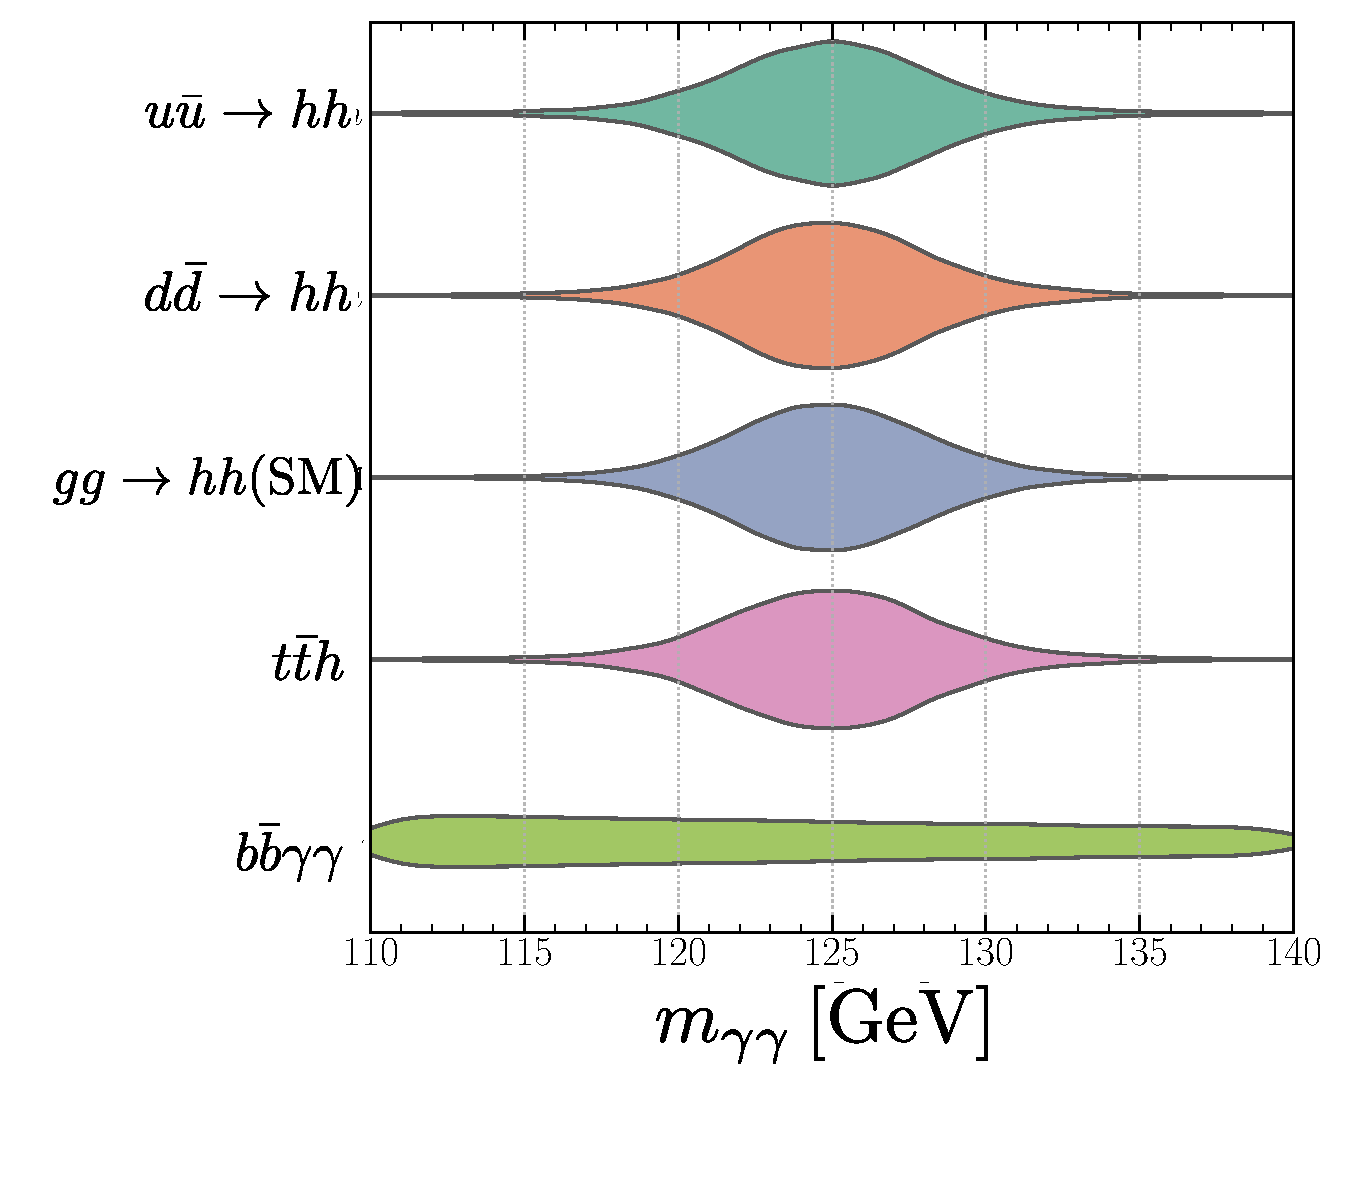
\includegraphics[width=0.35\textwidth]{fig/shape-MAA} 	\hspace*{0.25 cm}
	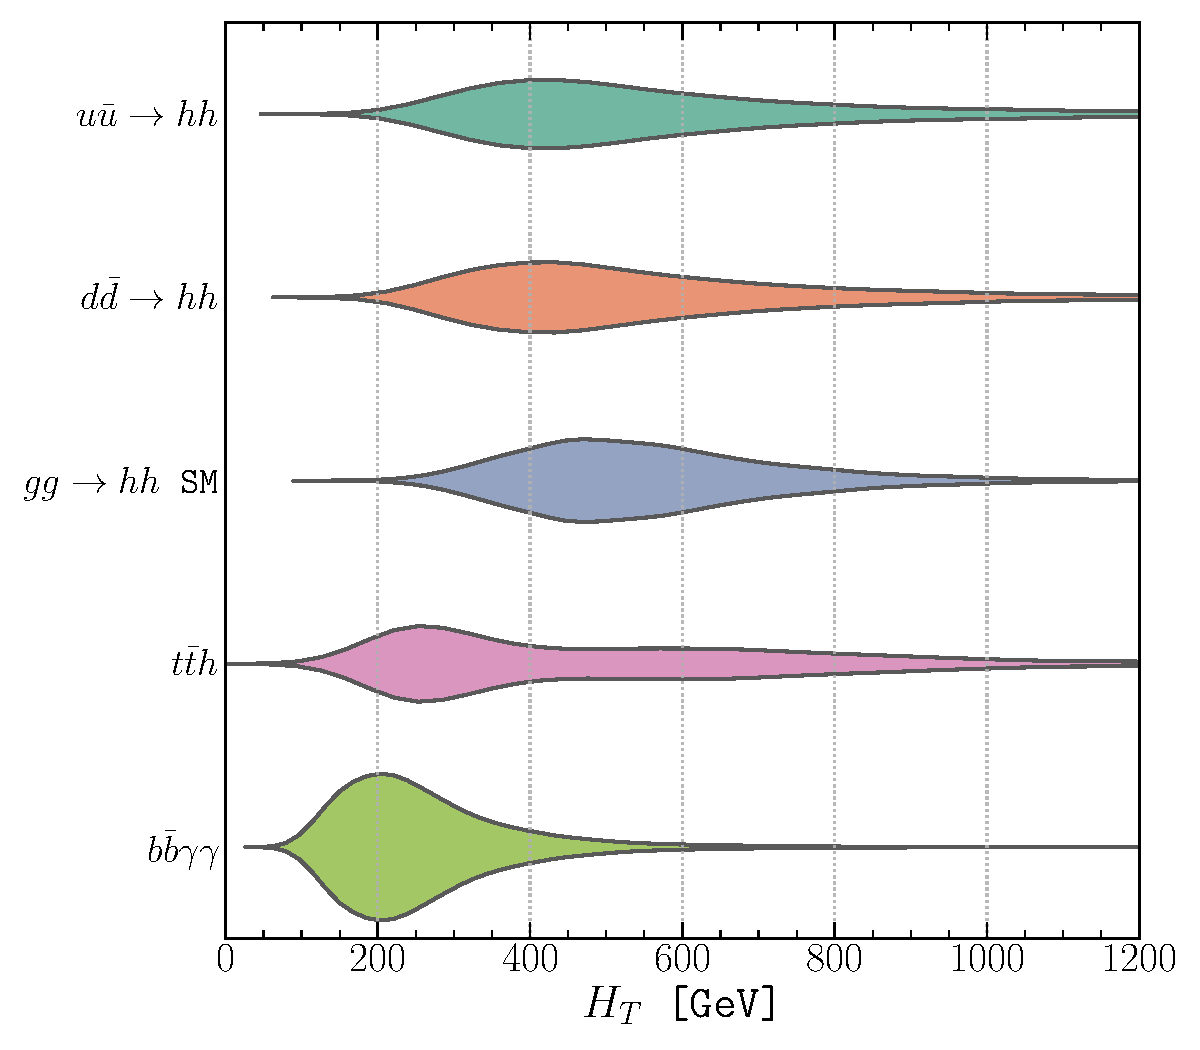
\includegraphics[width=0.35\textwidth]{fig/shape-HT}  \\
		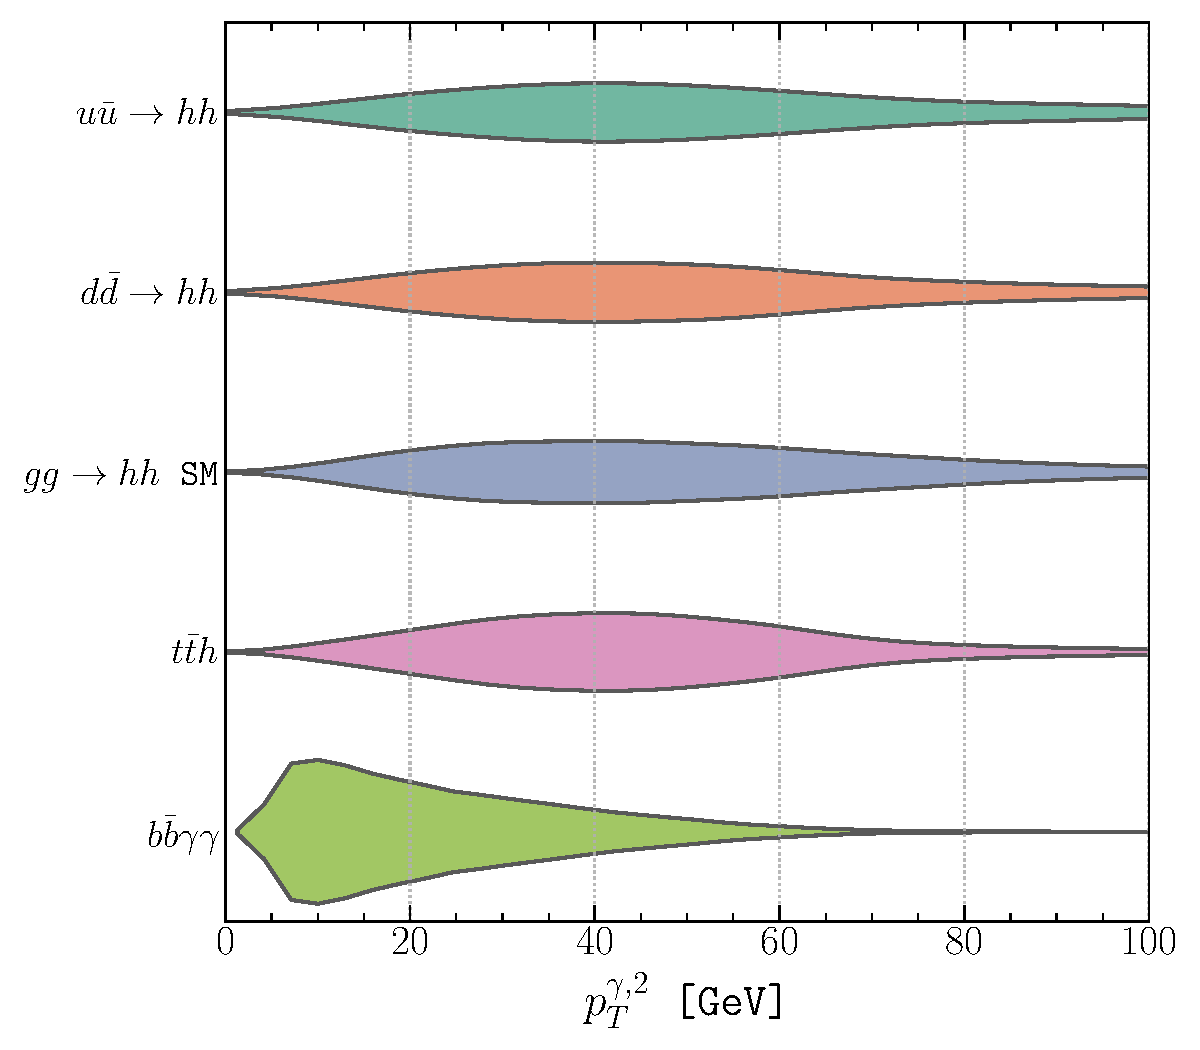
\includegraphics[width=0.35\textwidth]{fig/shape-PTA2} \hspace*{0.25 cm}
		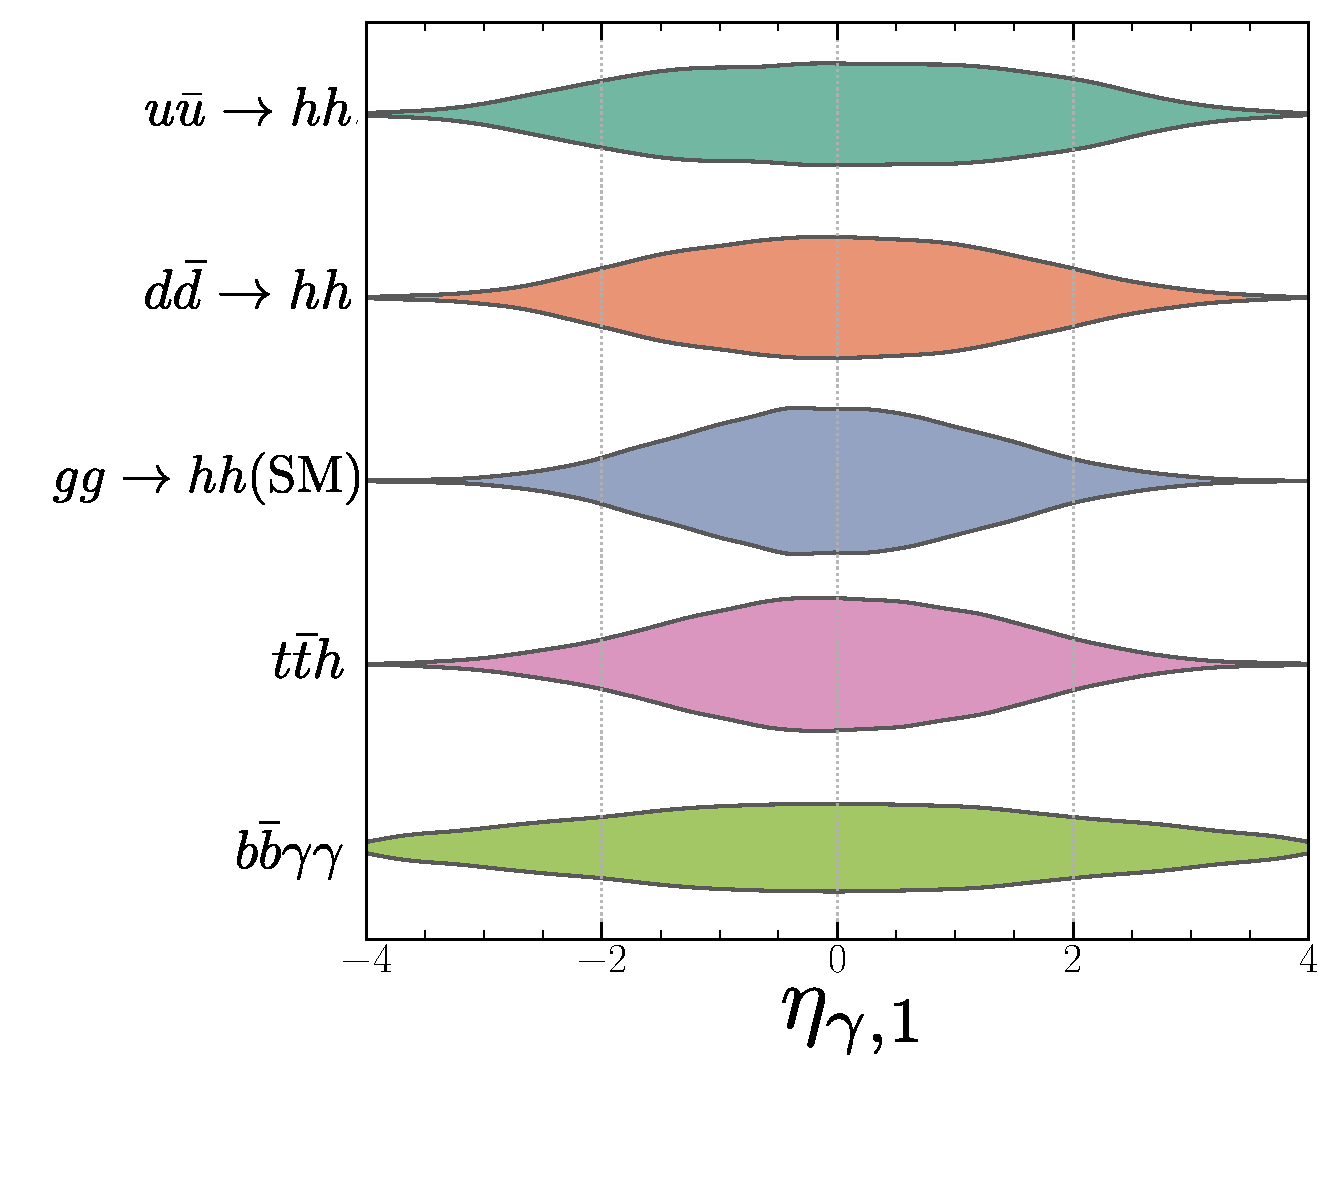
\includegraphics[width=0.35\textwidth]{fig/shape-ETAa1} 
	\caption{The . }
	\label{fig:voilen}
\end{figure}  

\begin{itemize}
	\item We show some well motivated BSM scenarios where light-quark Yukawas can be enhanced simultaneously with the Higgs trilinear coupling.
	\item We perform an interpretable machine learning analysis based on boosted decision trees and Shapley values, a measure derived from Coalition Game Theory to extract signal significance to get a better handle on the measurement of light-quark Yukawas.
	\item We perform simultaneous fits for several combinations of light-quark Yukawa couplings and the Higgs trilinear coupling.
\end{itemize}

We show in \autoref{sec:EFT} the relevant EFT operators for the di-Higgs processes, discuss flavor bounds and minimal flavor violation (MFV). Then we introduce in \autoref{sec:Model} the concept of aligned flavor violation (AFV), and various "concrete" examples realising large enhancement to light yukawa while evading flavor bounds. We then study the leading contributing channels with simulation details explained in \autoref{sec:Sim}. Further we discuss in \autoref{sec:kinematics} the multivariate analysis and interpretable machine learning approach we adopt. We present prospected results in \autoref{sec:hadronC} at the HL-LHC and FCC. In \autoref{sec:Sum} we summarize our main findings.

\begin{figure}[t]
	\centering
	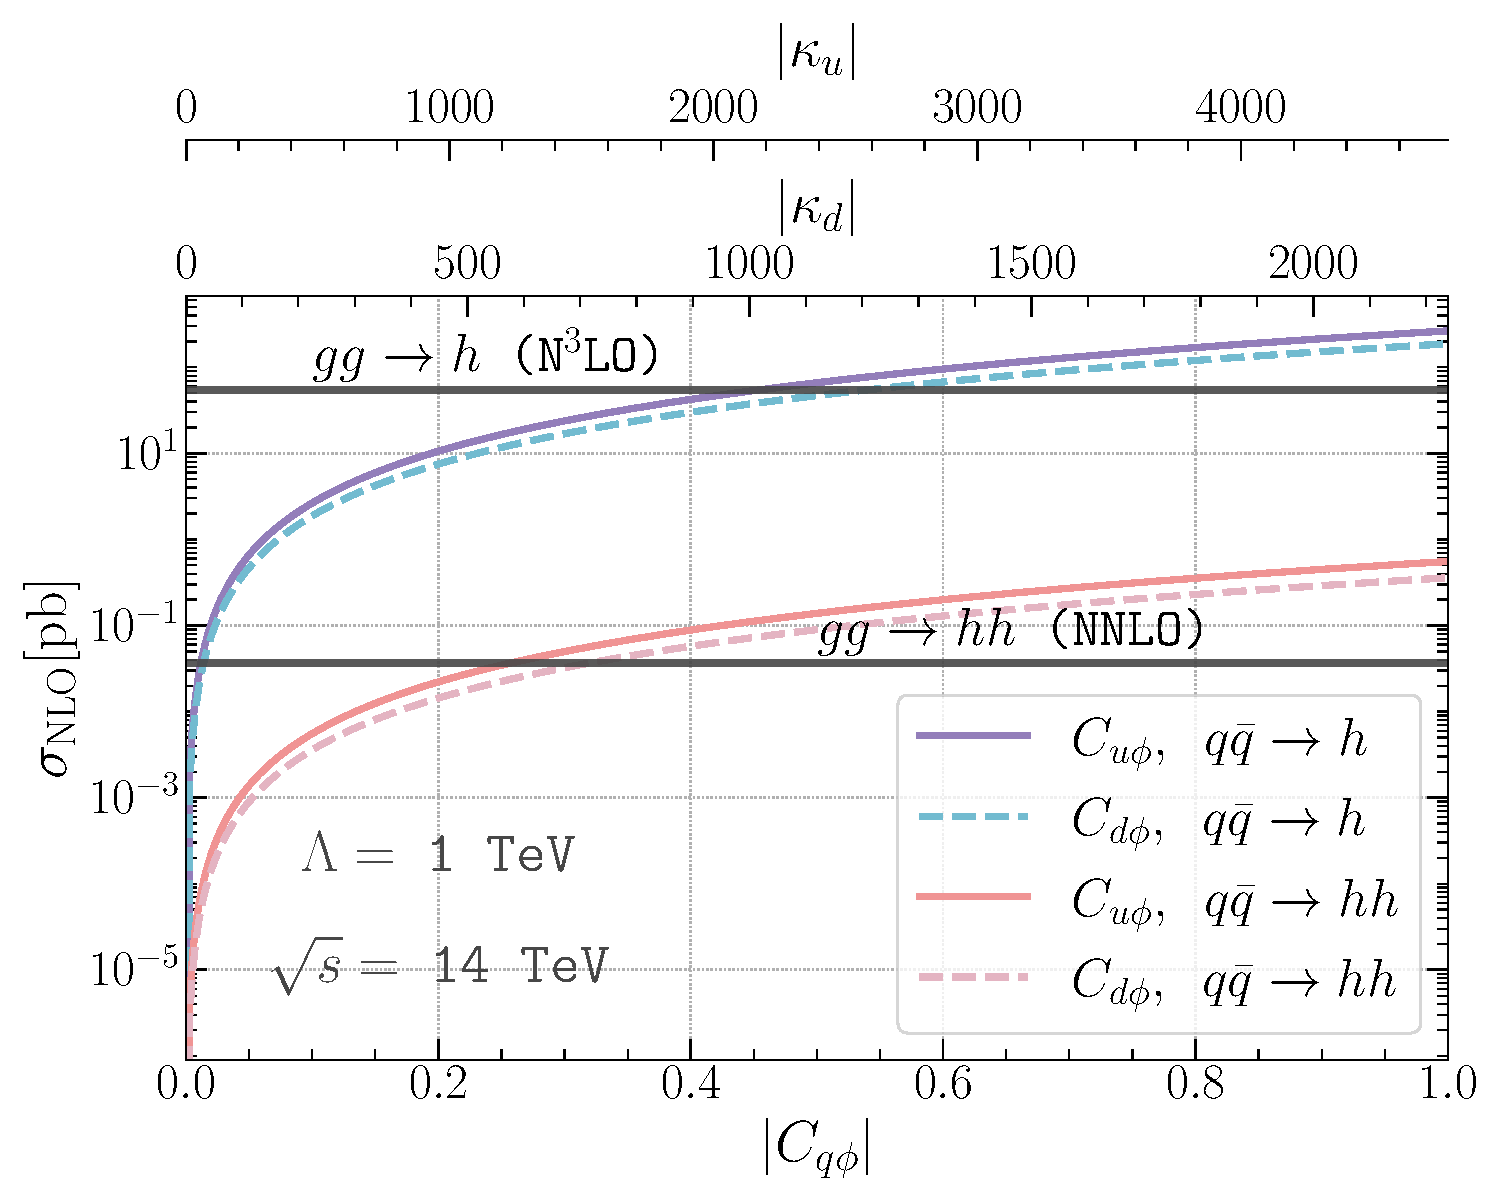
\includegraphics[width=0.75\textwidth]{fig/pph_hh_14Tev.pdf}
	\caption{\it The production cross-section of single Higgs and di-Higgs at $14$ TeV from the quark anti-quark annihilation $q\bar{q}A$ as a function of the Wilson coefficients $C_{u\phi}$ and $C_{d\phi}$ versus the SM gluon fusion cross-sections (the horizontal solid line for $gg \to h$ and the dashed-dotted one for $gg \to hh$). One can observe that for values of $C_{u\phi}=0.22\, (0.43)$ and $C_{d\phi}=0.26\, (0.47)$ the $q\bar{q}A$ channel becomes the dominant di-Higgs (single Higgs) production channel. The UV scale is set to $\Lambda = 1$ TeV. }
	\label{fig:pphhvsh}
\end{figure} 

In the general framework of SMEFT, additional assumptions on UV-motivated flavor structure avoids stringent low energy FCNC and EDM bounds, making collider probe on the Yukawa and related Wilson coefficients competitive and relevant. See a recent overview of Yukawa coupling bounds from flavor and collider Higgs data, in the SMEFT framework given certain flavor structure. \cite{Alonso-Gonzalez:2021tpo}

The single Higgs production and decay channels as measured currently already provide indirect bounds on the light quark Yukawa couplings from global fit. The main sensitivity comes from enhancement to the production when $q\bar q$ fusion of the Higgs become comparable to ggF channel when the corresponding light-quark Yukawa is sufficiently enhanced. Secondly, there is additional overall "dilution" factor from the modified Higgs total width, for a final state of a specific (non-"light-jet") decay channel.
In the case of di-Higgs, the $q\bar q hh$ contact interaction become important for the di-Higgs production, and could become dominant production channel over the SM gluon fusion channel through loop. The sensitivity thus achieved to the corresponding light-quark Yukawa in the SMEFT framework is better compared to that from single Higgs inclusive observable, and could even be competitive to single Higgs differential studies, as will be shown from our study.

%\zhuoni{Need to absorb/combine with Lina's discussion around \autoref{fig:pphhvsh} in \autoref{sec:Sim} of inclusive rate and Yukawa constraints comparing single and di-Higgs in SMEFT and SM.}
%\rg{I did not touch anything here but I think we should also write a few sentences on how the couplings we considered can be tested elsewise.}

%%%%%%%%%%%%%%%%%%%%%%%%%%%
\subsection{Considerations of experimental constraints}
%%%%%%%%%%%%%%%%%%%%%%%%%%%
For the 2HDM model, there are three main scenarios from the experimental searches point of view, in which one can obtain enhancements to light-quark Yukawa couplings. In the first scenario, the heavy Higgs $H$ has a small mass~$m_H <2$ TeV. Experimental resonance searches rules out this scenario where the resonant Higgs pair production is enhanced significantly due to the decay~$ H\to hh$, as the trilinear $Hhh$ coupling scales as~\cite{Egana-Ugrinovic:2021uew}
\begin{equation}
	g_{Hhh}\approx \frac{m_H^2}{v^2} \cos(\beta-\alpha).
\end{equation}
In the second scenario, we have a heavier $H$ but a large $Hq\bar{q}$ coupling. Here, the dijet resonance searches from $H\to jj$ decay, provides the strongest constraints. Lastly, when we consider a heavy $H$ and $Hq\bar{q}$  not excluded by di-jet searches we lie within the EFT limit and non-resonant Higgs pair production discussed in this paper gives us the dominant constraints.

In the 2HDM with AFV or SFV, there is an interplay between light quark Yukawa and the Higgs trilinear self-coupling. This comes from the alignment parameters $\alpha$ and $\beta$, as we see in equations~\eqref{Hqq} and~\eqref{lambda6}. For example, when the mass of $H$ is allowed to be very large $m_H >4$ TeV, enhancement to light-quark Yukawa couplings would be completely constrained from the bound on the Higgs self-coupling provided the 2HDM potential is tuned to avoid triviality and perturbativity bounds. 

%Currently, the improved experimental measurement of $D$-meson mixing \cite{LHCb:2021ykz} or decay may still allow for sizeable enhancement of the down-type light-quark Yukawa given the large non-perturbative theory uncertainty dominating $\Delta F=2$ transitions in the $D$ meson system. Measurement from $K$- and $B$-meson mixing and decays instead put stronger bounds on allowed enhancement to up-type quark Yukawa couplings
%This means that in these models large deviations in the Higgs couplings to down quarks can be achieved easier than in the up-sector. We emphasize again that simultaneously large deviations of the up- and down-quark Yukawa couplings are not possible.\la{why ?}
%%%%%%%%%%%%%%%%%%%
%The largest deviations in the light-quark Yukawa couplings are obtained for heavy Higgs boson masses within the discovery range of the LHC, while in the EFT limit (assuming a heavy Higgs boson mass of $> 2.5\text{ TeV}$), deviations of the light-quark Yukawa coupling of up to a factor of 100 can be obtained. For large coupling between the light quarks and the heavy Higgs~$H$, the dijet searches $H\to jj$ dominate the bounds. For relatively light $H$, i.e. $m_H < 1$ TeV and smaller coupling to the light quarks, the resonant Higgs pair production  from $ H \to hh$ gives the most stringent bounds. However, if neither of the cases apply, the bounds obtained from our analysis will be the most stringent ones. It should be noted that this region in the parameter space requires large couplings which could potentially lead to Landau poles. A concrete statement on the appearance of the Landau poles  depends on the concrete parameter set and the UV dynamics.




%\zhuoni{Ref. \cite{Bar-Shalom:2018rjs} discuss mainly mixing between the SM and their corresponding VLQs through the scalar sector through yukawa couplings. It's worth pointing out that mixing through the electroweak gauge coupling introduce further contribution to the SM-like loop-induced FCNCs, which is now not protected by the small quark mass in the loop or GIM mechanism. This however can again be suppressed by alignment assumptions on the additional flavor structure introduced from the VLQ's weak interaction. }
%Tree level suppression of FCNC is however not enough to suppress FCNC process induced at loop-level, which is suppressed in the SM (and proportionally in MFV) by the GIM mechanism. For example, the lowest order down-sector FCNC bilinear for the VLQ model can be written as, 
%\begin{equation}
%	\bar d_i^\dagger \lambda_{Qd} V^*_{CKM} |M_{U}^2| \lambda_{Qd} \bar d_j.
%\label{eq:vlq_gim}
%\end{equation}
%The $U,D$ mass matrices here are diagonal with aligned flavor symmetry. It could be seen as induced by  loop-induced FCNC diagrams such as shown in \autoref{fig:gim}, replacing the quark in the loop with its VLQ counter-part. 

%\begin{figure}[t]
%\centering
%\includegraphics[width=0.35\textwidth]{fig/kaon_gim.jpg}
%\caption{\it The loop-induced FCNC that could be enhanced when replacing the loop particle with a weakly charged VLQ.}
%\label{fig:gim}
%\end{figure}  

%An estimate of the correction to FCNC from \autoref{eq:vlq_gim}  would be of order $\sin\theta_c\cos\theta_c(M_{U1}^2-M_{U2}^2)$, neither protected by light-quark Yukawa or GIM mechanism. Whereas in the SM case it is proportional and suppressed with $\mathcal{O}(\frac{m_c^2-m_u^2}{m_W^2})$.
%\textcolor{red}{RG: define the meaning of the parameters}
%\textcolor{red}{I am still a little confused about this loop contribution. Looking at the EFT four fermion operators it seems to me there is always a Yukawa suppression in EFT. }
%\par
%In general we note, that while a UV explanation of a flavour-aligned generation of the operators in \autoref{eq:EFTop} is certainly highly non-trivial due to the interplay with various flavour constraints, we would like to emphasize that there is no theoretical or experimental constraints forbidding large Yukawa modifications of the light quark Yukawa couplings. While for other couplings (see e.g. for the trilinear Higgs self-coupling modification in~\cite{DiLuzio:2017tfn, Falkowski:2019tft, Chang:2019vez}) theoretical arguments like perturbative unitarity can be invoked, for the light-quark Yukawa coupling they would not lead to any strong constraint, keeping in mind that we already know that they are smaller than the Yukawa couplings of the third generation fermions. Furthermore, the radiative generation of FCNCs in diagrams with the Higgs boson under the assumption of flavour alignment, while not being radiatively stable, is still suppressed by two light-quark mass insertions.

%We have not discussed the trilinear Higgs self-coupling within the proposed models but one can easily imagine additional scalars (e.g. singlet states) that do not affect the flavour structure but dominantly the Higgs self-couplings. In such models a simultaneous modification of the trilinear Higgs self-coupling and enhanced light Yukawa couplings can be realised.
%\zhuoni{To summarise the discussion above, compared to MFV, AFV provides mechanism for an enhanced light yukawa while avoiding tree level FCNC terms.
	%However AFV in general does not suppress SM-like charge current induced loop level FCNC which in the SM is of order $V_{CKM}*\frac{\Delta(m_q^2)}{M_W^2}$, protected by the so-called GIM-mechanism. As evaluated in the SFV-2HDM example \cite{Egana-Ugrinovic:2019dqu}, a $y_b^{\rm SM}$ sized first two generation light quark yukawa gives a FCNC contribution $\sim V_{CKM}*\frac{(mb^2)}{\Lambda^2}$, which can be comparable to or overwhelming the SM contribution. Indeed the enhanced light quark yukawas in the model are most strongly constrained by meson decay/mixing data. On the other hand, AFV with additional flavor sector and structure, as in the case of the VLQ model\cite{Bar-Shalom:2018rjs}, could suppress the contribution with $V_{CKM}*V'_{CKM}$. By setting the new flavour structure orthogonal to SM $V_{CKM}$, FCNC can be further avoided or suppressed to higher loop order.}


From the discussion in this section we see that several models are present in the literature that are able to accommodate for large deviations of the light-quark Yukawa couplings from their SM values while avoiding excessive contributions to FCNCs that are well measured and particularly limiting for models with additional flavour structures due to the implementation of AFV or SFV. The primary new physics deviation, complementary to direct searches, in the presented models will show up in the modification of the light quark Yukawa couplings. Armed with this knowledge, we motivate a study of how light-quark Yukawa couplings can be constrained at future experiments from Higgs pair production.


%%%%%%%%%%%%%%%%%%%%%%%%%%%
% \section{Signal and background simulation for the final state $b\bar{b}\gamma \gamma$}
\section{Events simulation for HL-LHC and FCC-hh}
\label{sec:Sim}
%%%%%%%%%%%%%%%%%%%%%%%%%%%
We consider the final state~$b \bar{b} \gamma \gamma$, as this channel has the most potential for Higgs pair searches~\cite{Cepeda:2019klc}. It has the ``clean'' $h \to \gamma \gamma$ decay, but also the other Higgs decay to $b$-quark pair is a channel with large branching ratio~$\sim 58\%$ and b-tagging capabilities for ATLAS and CMS are continuously improving.
\begin{table}[h!]
	\centering
	\begin{tabular}{cccc}
		\specialrule{.8pt}{0pt}{0pt}
		Channel	        &LO $\sigma$ [fb]	&NLO $K$-fact	&6$\inab$ [\#evt @ NLO]   \\ %& 2$b$-jets[\%]  \\ 
		\specialrule{.8pt}{0pt}{0pt}
		$y_b^2$	        &0.0648	            &1.5	    &583                \\%&7.7\%  \\
		$y_by_t$        &-0.00829	        &1.9        &-95                \\%&4.0\%	\\
		$y_t^2$	        &0.123	            &2.5	    &1,840              \\%&12\%	\\
		$Zh$	        &0.0827	            &1.3	    &645                \\%&21\%   \\
		$\sum\bbh$	    &0.262	            &-	        &2,970              \\%&-      \\
		$\bbaa$	        &12.9	            &1.5	    &116,000            \\%&14\%	\\
		$t\bar th$	    &1.156	            &1.2	    &6,938              \\%&42\%	\\
		%$hh_{\rm SM}$	&0.567	\la{0.053}            &1.72	    &3,492  \la{316}              \\%&32\%	\\ 
		\specialrule{.8pt}{0pt}{2pt}
	\end{tabular}
	\caption{\it SM cross-section for the main background processes at 14\,$\tev$ with 6\,$\iab$ data at the HL-LHC, and the number of events after the basic cuts as defined in \autoref{eqn:bcuts}. For $\bbh$ production, the Higgs boson is decayed to a pair of photons. The total production of Higgs associated with $b\bar{b}$ is denoted by $\sum\bbh$ and is the sum of the top four channels.
	}
	\label{tab:xsec14}
\end{table}

\begin{figure}[t]
	\centering
	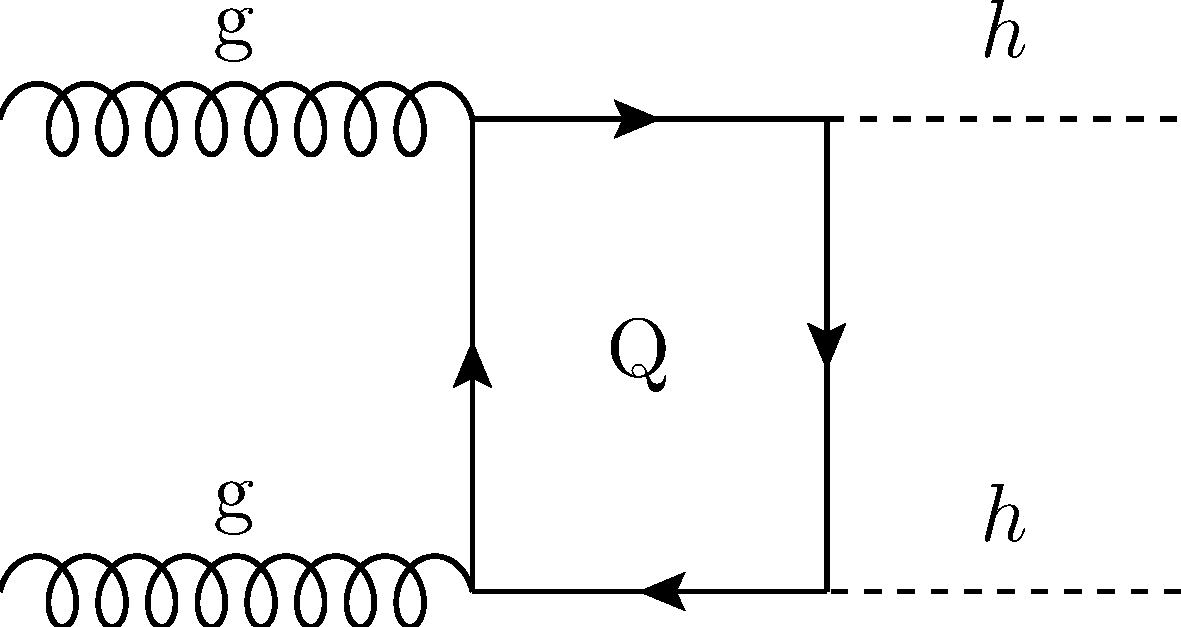
\includegraphics[width=0.25\textwidth]{fig/ggfbox} 	\hspace*{0.5 cm}
	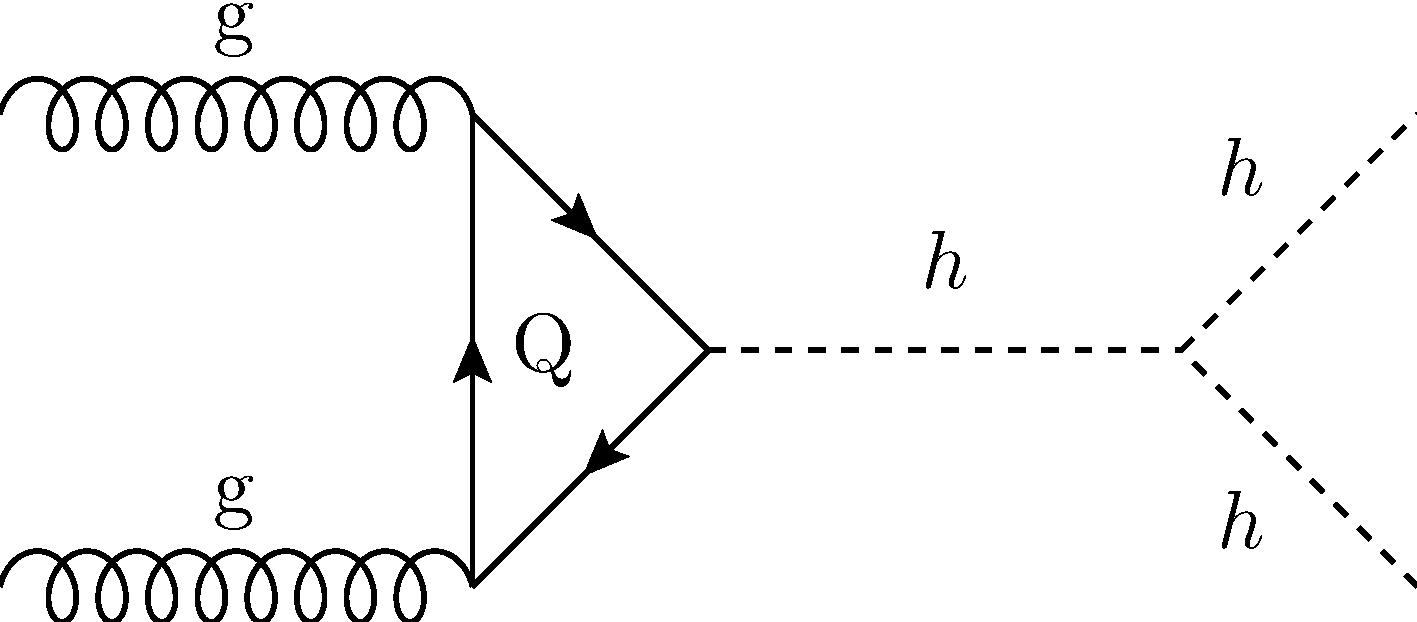
\includegraphics[width=0.29\textwidth]{fig/ggftri}
	\caption{\it The cross-section of the $gg$F channel can be decomposed into three subprocesses based on its dependence on the trilinear coupling $\lambda$. The triangle topology depends on $\lambda^2$, the box one does not depend on it and the interference amongst the latter two is linear in $\lambda$. }
	\label{fig:ggfsub}
\end{figure}  
\begin{figure}[t]
	\centering
	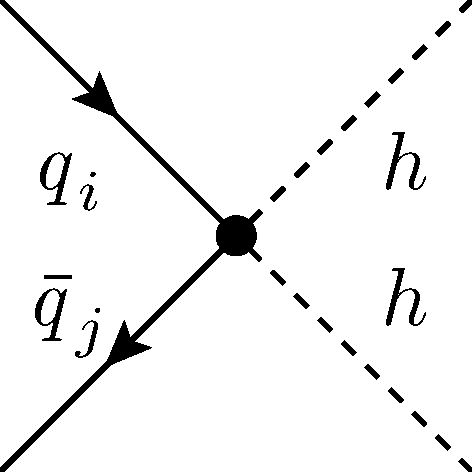
\includegraphics[width=0.125\textwidth]{fig/qqh_dim6}
	\hspace*{0.5 cm}
	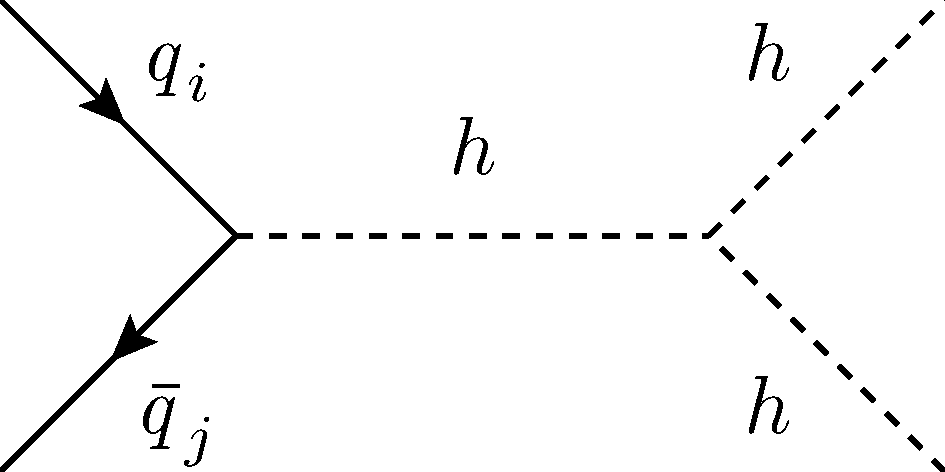
\includegraphics[width=0.25\textwidth]{fig/qqh_higgs_prpg}
	\caption{\it The dominant Feynman diagrams for the quark anti-quark annihilation~($q\bar q$A)  production of Higgs pair, via the SMEFT operator $ \mathcal O_{q\phi}$. }
	\label{fig:qqa}
\end{figure}

To be able to study the effects of enhanced light-quark Yukawa couplings or Higgs trilinear coupling, we need to simulate events for HL-LHC and FCC-hh which we use to train a machine learning model to identify the signal from the background. We consider the $b\bar bh$, $t\bar th$, $b\bar b \gamma\gamma$ processes as the main sources of background for the $hh$ signal. For the $b\bar bh$ processes, the contributions proportional to $y_b^2$, $y_by_t$ and $y_t^2$ are simulated separately with $y_b$ running effects. The details of the simulation can be found in Ref.~\cite{Grojean:2020ech}. The $Zh, Z\to b\bar b$ events are generated at leading order (LO), then scaled to NLO by $K$-factors, defined as the ratio of higher order cross section over its LO counterpart. The $K$-factors were taken from $t\bar{t}h$~\cite{Beenakker:2001rj}, $b\bar b \gamma\gamma$~\cite{Fah:2017wlf}, $Zh$~\cite{Campanario:2014lza} and the remaining part of the $b\bar bh$ processes from~\cite{Dawson:2005vi}. The Higgs particles are further decayed to $\gamma\gamma$ following the Higgs cross-section working group recommendations~\cite{LHCHiggsCrossSectionWorkingGroup:2016ypw}. The parton-level results are showered using \texttt{Pythia 8.3}~\cite{Sjostrand:2014zea} and a detector simulation is done using \texttt{Delphes 3}~\cite{deFavereau:2013fsa}. To be inclusive and to explore the capabilities and importance of the full detector coverage, no generator-level cuts were applied on these processes except for the $b\bar b \gamma\gamma$ processes to avoid divergences. These minimal generator-level cuts for $b\bar b\gamma\gamma$ are
\begin{equation}
	\begin{aligned}
		& Xp_T^b>20\,\gev, \\
		\textrm{generator level cuts:}\qquad& \eta_\gamma<4.2,~ \Delta R_{b\gamma}>0.2, \\
		& 100< m_{\gamma\gamma} \,(\gev) < 150.
	\end{aligned}
\end{equation}
Here $Xp_T$ implies a minimum $p_T$ cut for at least one $b$-jet. 
After the showering and detector simulation, further basic selection cuts were applied to select events with
\begin{equation}
	\textrm{basic cuts:}\qquad
	\begin{array}{l}
		n_{\mathrm{eff}}^{bjet}\geq 1,~n_{eff}^{\gamma jet} \geq 2,\\
		p_T^{bjet}>30\,\gev,~p_T^{\gamma jet}>5\,\gev,\\
		\eta_{bjet,\gamma jet}<4,~ 110\, \gev < m_{\gamma_1\gamma_2} < 140\,\gev,
	\end{array}
	\label{eqn:bcuts}
\end{equation}
and $n_{eff}^{b/\gamma jet}$ representing the number of $b/\gamma$-jets that pass the basic selection. The cross-section, $K$-factors, number of events with 6ab$^{-1}$ luminosity at 14 TeV are given in \autoref{tab:xsec14}. 

\begin{table}[t]
	\centering
	\begin{tabular}{ccccc}
		\toprule
		Channel	        &LO $\sigma $ [fb]	&$K$-fact.	&Order&6$\inab$ [\#evt @ order]   \\
		\midrule
		$\hhtri$	        &  $7.288 \cdot10^{-3}$    & 2.28 &\multirow{3}{*}{NNLO}   &  96   \\ 
		$\hhbox$            & $0.054$    & 1.98 &  & 680   \\ 
		$\hhint$            &$-0.036$    & 2.15 &  &-460   \\ 
		$\uuA$ $(C_{d\phi}=0.1)$ &  $2.753$    & 1.29&\multirow{2}{*}{NLO} &  28   \\ 
		$\ddA$ $(C_{u\phi}=0.1)$ &  $4.270$    & 1.30 & &  43   \\ 
		\bottomrule
	\end{tabular}
	\caption{  The LO cross-section for di-Higgs production at the HL-LHC for 6$\inab$ of data multiplied by the $hh \to b \bar b \gamma \gamma$ branching ratio, $K$-factors (taken from \cite{ deFlorian:2021azd} for the gluon channels and \cite{Alasfar:2019pmn} for the quark channels) and the number of events after the basic cuts for the separated gluon fusion~($gg$F) and quark annihilation~($\qqA$) at $\sqrt{s}=14$ TeV. }
	\label{tab:kfact}
\end{table}

While the backgrounds are generated using \texttt{MadGraph\_aMC@NLO}~\cite{Alwall:2014hca}, the $hh$ signal is separated into two main channels. The first is the gluon-fusion~($gg$F) channel which is the dominant channel in the SM and which can be further decomposed into three subprocesses based on their dependence on the Higgs trilinear self-interaction, $\lambda$, as seen in \autoref{fig:ggfsub}. Amongst these subprocesses, the first is the amplitude squared of the contribution from the triangle diagram. It is proportional to $\lambda^2$. The second is the squared amplitude of the contribution from the box diagram that does not depend on the trilinear coupling. The third is the contribution from the interference between the triangle and box diagrams, which is proportional to~$\lambda$. Using this separation allows us to remove the dependence of the total $K$-factor for $hh$ production on rescaling of the trilinear Higgs coupling~\cite{Heinrich:2019bkc}. The individual $K$-factors for each of the subprocesses are independent of the rescaling of the trilinear Higgs coupling making our analysis computationally much simpler. The $gg$F process is generated using the \texttt{HH} production program implemented in \texttt{POWHEG}~\cite{Heinrich:2017kxx,Heinrich:2019bkc,Heinrich:2020ckp}, which has been modified to separate the individual contributions from the three diagrams. The cross-section for these individual contributions and the corresponding $K$-factors can be found in \autoref{tab:kfact}. 
%\rg{What about fakes? I remember we had some discussion about fake backgrounds some time ago...}\la{I am not sure what do you mean by fakes here.. do you mean $c\bar c \gamma \gamma$?  }
%\rg{I think we need to cite here all the works on NLO corrections in HH}\la{Done, but do you want me to describe the references in more detail ?} \rg{reminder to me, select the relevant ones after we clarfied of using NNLO or not...}
%\cite{Dawson:1998py,Shao:2013bz,Maltoni:2014eza,Borowka:2016ehy,Borowka:2016ypz,Jones:2017giv,Baglio:2018lrj,Bonciani:2018omm}, see also~\cite{deFlorian:2013jea,deFlorian:2013uza,Grigo:2014jma,deFlorian:2015moa,deFlorian:2016uhr} for beyond NLO calculations, and for QCD corrections to di-Higgs within EFT's see~\cite{Grober:2015cwa,Grober:2017gut,deFlorian:2017qfk,Buchalla:2018yce}

The other main process, the quark anti-quark annihilation~($q\bar q$A), is strongly suppressed in the SM for first generation quarks since the SM Yukawa couplings are proportional to the mass of the considered quark flavour. However, since this channel is a tree-level process, with sufficient large enhancement factors of the light quark Yukawa coupling, it becomes dominant as shown in \autoref{fig:pphhvsh}. The $q\bar q$A cross section scales like $\tilde{C}_{q\phi}^2/\Lambda^4$,  while the gluon fusion production cross-section remains almost unchanged. Therefore, for constraining enhancements of the light-quark Yukawa, we consider this channel as the signal and the $gg$F channel as part of the background. The $q\bar q$A process is generated with~\texttt{MadGraph\_aMC@NLO} with a UFO model created with \texttt{FeynRules}~\cite{Alloul:2013bka}. Samples for both up- and down-quark initiated $q\bar q$A processes is generated. For all the $hh$ signals, the samples are generated at LO and later scaled by the NLO $K$-factors given in \autoref{tab:kfact}. The $K$-factors are obtained from ref.~\cite{Buchalla:2018yce} for the gluon fusion process in EFT and adapted from \cite{Dicus:1998hs,Balazs:1998sb, Harlander:2003ai} as described in \cite{Alasfar:2019pmn} for the $q\bar q$A channel. Moreover, the two Higgs bosons are decayed to $b\bar b$ and $\gamma\gamma$ respectively, with \texttt{Pythia 8.3} and then showered. The same detector simulation and basic cuts as for the background are then performed. In addition, the same sets of parton distribution function (\texttt{NNPDF31\_nlo\_as\_0118\_nf\_4}) are used for the signal and the background, implemented via \texttt{LHAPDF}~\cite{Buckley:2014ana}. The calculation of the Higgs full width and branching ratios is done using a modified version of~\texttt{Hdecay}~\cite{Djouadi:1997yw,Djouadi:2018xqq} to include the new SMEFT operators $\mathcal{O}_{q\phi}$. It should be noted, that in both di-Higgs production and decay calculation, the light-quark masses are set to zero. However, when converting between SMEFT and $\kappa$-formalism, the $\overline{\mathrm{MS}}$ quark masses are used, in accordance to the PDG.

For FCC-hh, almost everything is done similarly after setting the energy to 100 TeV and the luminosity to 30 ab$^{-1}$. Since we do not have all $K$-factors available at a collider energy of 100 TeV we rescaled the LO samples by the same ones as for HL-LHC. We note that we explicitly checked that at least within the SM, for Higgs pair production via gluon fusion the difference is of $\mathcal{O}(1\%)$~\cite{Maltoni:2014eza} and hence small.




%%%%%%%%%%%%%%%%%%%%%%%%%%%
\section{Exploring higher dimensional kinematic distributions}
\label{sec:kinematics}
%%%%%%%%%%%%%%%%%%%%%%%%%%%

After detector simulation and jet definition, we have a final state of two photon jets and at least one $b$-jet, where the two photons reconstruct back to a real scalar Higgs mass for all the $\bbh$ channels. We first define and evaluate a comprehensive set of kinematic observables as the following:
\begin{itemize}
	\setlength{\itemsep}{0pt}
	\item $p_T^{b_1}$, $p_T^{b_2}$, $p_T^{\gamma_1}$, $p_T^{\gamma\gamma}$, 
	\item $\eta_{b_{j1}}$, $\eta_{b_{j2}}$, $\eta_{\gamma_1}$, $\eta_{\gamma\gamma}$,
	\item $n_{bjet}$, $n_{jet}$, $\Delta R_{\rm min}^{b\gamma}$, $\Delta \varphi_{\rm min}^{bb}$, 
	\item $m_{\gamma\gamma}$, $m_{bb}$, $m_{b_{1} h}$, $m_{b\bar b h}$, $H_T$.
\end{itemize}
$p_T^{{b/\gamma}_{1,2}}$ and $\eta^{{b/\gamma}_{1,2}}$ are the $p_T$ and rapidity for the tagged leading and sub-leading $b/\gamma$-jets (in our definition the subleading $b$-jet could be a null four-vector since we require one $b$-jet inclusive), $n_{bj}$ is the number of tagged and passed $b$-jets. $\Delta R_{\rm min}^{b\gamma}$ and $\Delta \varphi_{\rm min}^{bb}$ are the minimum $R$-distance and $\varphi$-angle between a tagged $b$-jet and a photon jet. The remaining variables are the invariant masses and $H_T$ is the scalar sum of the transverse mass of the system. We shall show in what follows, that it is not necessary to be very selective about the kinematic variables one chooses to use in the analysis. What is necessary is that all possibly useful kinematic variables are included. As can be seen from the list above, some of the variables seem to be interdependent and, probably, highly correlated. The beauty of using interpretable machine learning is that a hierarchy of importance for the variables will be built during the analysis using an over-complete basis of collider observables from which the most important ones can be chosen to fine tune the analysis. 


%%%%%%%%%%%%%%%%%%%%%%%%%%%
\subsection{Interpretable machine learning}
\label{sec:BDT}
%%%%%%%%%%%%%%%%%%%%%%%%%%%

Rule-based machine learning algorithms have for long been used as the gold standard for signal to background discrimination in a wide variety of particle physics analyses. They are known to outperform neural networks in terms of simplicity of implementation, computational resources required and accuracy in modelling the underlying distributions.\footnote{Nevertheless, we tested a deep neural network built with Tensorflow~\cite{tensorflow2015-whitepaper} and found no improvement in the classification accuracy.} In addition, rule-based algorithms, such as decision trees, are more transparent as far as the signal vs.~background separation is concerned. Placing emphasis on interpretability in multivariate analyses, we chose to work with Boosted Decision Trees (BDT). However, interpretability of a machine learning algorithm requires more than just a choice of an interpretable model. The conditions are:
\begin{itemize}
	\itemsep0em
	\item A variable set that is easily interpretable in terms of the dynamics being studied.
	\item A machine learning algorithm that is more transparent and not a complete black box.
	\item A method for interpreting the model and attribute variable importance to understand how the algorithm models the underlying distributions.
\end{itemize}
Choosing to work with BDTs just satisfies the second condition. We work with the BDT algorithm implemented in XGBoost~\cite{10.1145/2939672.2939785}, a publicly available scalable end-to-end boosting system for decision trees. We follow the normal procedures for training and testing the BDT with simulated data. To satisfy the first condition we chose to work with high level kinematic variables that are representative of the process instead of working with four-vectors. The disadvantage of working with kinematic variable is that a complete set cannot be defined for a particular process unlike the four-vectors associated with the process. So, in principle, a large number of kinematic variables can be formulated and used in a multivariate analysis. While the number is never too large for any implementation of BDTs, having a large set of variables clouds the understanding of which ones are important for orchestrating the signal separation from the background. This is where the third point listed above is important. Variable importance attribution is a way to ``short-list'' only those variable that play an important role in predictive power of the classification (or regression) problem. There are several measures of variable importance used in machine learning like Gini or permutation based measures~\cite{Breiman2001,JMLR:v20:18-760}, local explanations with surrogate models~\cite{10.1145/2939672.2939778} etc., to name a few. However, these suffer from inconsistencies or fail to provide a global explanation of the model~\cite{NIPS2017_7062}. 

To build a mathematically consistent procedure for variable importance attribution we use Shapley values~\cite{shapley1951notes} from Coalition Game Theory. Formulated by Shapley in the mid-20$^{th}$ century, Shapley values formulate an axiomatic prescription for fairly distributing the payoff of a game amongst the players in a $n$-player cooperative game. When applied to machine learning, Shapley values tell us how important the presence of a variable is in determining a certain category (like signal or background) when compared to its absence from the multivariate problem being addressed. The process naturally and mathematically lends itself to studying the correlations between different variables since all possible combinations of variables can be taken out of the game to check the outcome.\footnote{More clarity on Shapley values and interpretable machine learning in general, along with their application can be found in \href{https://christophm.github.io/interpretable-ml-book/}{Interpretable Machine Learning } by Christoph Molnar~\cite{molnar2020interpretable}.} A more detailed discussion of the application of Shapley values to signal vs.~background classification problems for particle physics can be found in Refs.~\cite{Grojean:2020ech,Alvestad:2021sje,Cornell:2021gut}. In this work we follow the same basic procedure as discussed in Ref.~\cite{Grojean:2020ech}. The importance of a variable in determining the outcome of a classification will be quantified by the mean of the absolute Shapley value, $\overline{|S_v|}$, larger values signifying higher importance. We will use the SHAP (SHapley Additive exPlanations)~\cite{NIPS2017_7062} package implemented in python based on Shapley values calculated exactly using tree-explainers~\cite{2018arXiv180203888L,Lundberg:2020vt}.


%%%%%%%%%%%%%%%%%%%%%%%%%%%
\section{The \texorpdfstring{$hh$}{hh} channel at future hadron colliders}
\label{sec:hadronC}
%%%%%%%%%%%%%%%%%%%%%%%%%%%

We would like to study the bounds on three specific couplings in this work. The first one being the Higgs trilinear coupling quantified by $C_\phi$ defined in \autoref{eq:EFTop} and the other two being the deformation of the first-family SM Yukawa coupling to the up and down quark defined as $C_{u\phi}$ and $C_{d\phi}$ in \autoref{eq:couplingsEFT} with $i=j=1$. 
We will not consider modifications of the second generation of quarks as their effects in di-Higgs production would be suppressed by the small parton distribution functions and are hence expected to be more pronounced using other methods for constraining them.
For ease of interpretation we will also present our results in terms of $\kappa_\lambda$, $\kappa_u$ and $\kappa_d$ which are simply the rescaling of the SM trilinear coupling and the light-quark Yukawa couplings of the up and down quarks, respectively. 
%These can be found in the appendix. 

In the BDT analysis we combine the $\bbh, (h\to\gamma\gamma)$ and $\tth, (h\to\gamma\gamma)$ channels into one category calling it $Q\bar Q h$ while the other (continuum) background channel, $\bbaa$, is treated as a separate category. For any analysis involving $C_\phi$, we need three separate categories for the triangle, box and interference terms of the $gg$F $hh$ production which we shall refer to as $\hhtri$, $\hhbox$ and $\hhint$, respectively. The $\qqA$ channels stands for two other categories, one each for probing the Wilson coefficients $C_{u\phi}$ and $C_{d\phi}$, respectively. However, the $q\bar q$A channels are not the only channels sensitive to $C_{u\phi}$ and $C_{d\phi}$. In fact the decay $h\to\gamma\gamma$, the production of the Higgs in the $gg$F channel and the width of the Higgs are modified by the size of $C_{u\phi}$ and $C_{d\phi}$~\cite{Alasfar:2019pmn}. Hence, these as well need to be taken into account. In what follows, we will refer to the two $q\bar q$A channels as $\uuA$ and $\ddA$ explicitly.

As we progress through the analysis we study the modification of one, two and three Wilson coefficients at a time. To extract just $C_\phi$ from the data we need to perform a five channel classification (two signal and three background modes including the $\hhbox$ contribution that is insensitive to modifications of $C_\phi$). To extract either $C_{u\phi}$ or $C_{d\phi}$ we have to perform a four channel classification taking the $gg$F channel as a single background mode.  To extract $C_\phi$ and one of $C_{u\phi}$ or $C_{d\phi}$ we need to perform a six channel classification. Lastly, to extract all three Wilson coefficients we will need a seven channel classification. All the codes and data necessary to reproduce the results we got from this interpretable machine learning framework are made available at a \texttt{Github} repository: \href{https://github.com/talismanbrandi/IML-diHiggs.git}{https://github.com/talismanbrandi/IML-diHiggs.git}.

To set the stage, we will define our measure of significance and how we estimate it. We first construct a confusion matrix from the predictions of the trained BDT. This is a $n\times n$ matrix, for $n$ channels. The sum of the elements in the $i^{th}$ row, $\sum_j N_{ij}$, gives the actual number of events produced in channel $i$ that would be generated in a pseudo-experiment with the projected luminosity corresponding to the actual experiment. The sum of the $j^{th}$ column, $\sum_i N_{ij}$, gives the number of events from channel $j$ predicted (including correct classifications and misclassifications) by the BDT in this pseudo-experiment. Hence the $(i,j)$ element of the matrix gives the number of events of the $i^{th}$ class that is classified as belonging to the $j^{th}$ class with $i\ne j$ signifying a misclassification. The significance of the $j^{th}$ channel given by $S/\sqrt{S + B}$, $S$ being signal and $B$ being background, can be defined as
\begin{equation}
	\mathcal{Z}_j=\frac{|N_{jj}|}{\sqrt{\sum_i N_{ij}}},
\end{equation}
where $i$ is the row index and $j$ is the column index. 

%\rg{It seems there is a copying mistake here! Let's check thatr there is not too much overlap to avoid an arXiv text overlap.}

The fact that machine learning algorithms can far outperform cut-and-count analyses is a bygone conclusion. Preliminary estimates of the HL-LHC reach for SM di-Higgs production can be found in~\cite{Cepeda:2019klc} and range from 4$\sigma$ to $4.5\sigma$ signal significance combining several channels and both the ATLAS and CMS measurements. The $\bbaa$ final state alone allows for a $\sim2.7\sigma$ measurement. In~\cite{Alves:2017ued} a more refined machine learning procedure using Bayesian Optimization has been suggested and it has been shown that, indeed, the measurement of a di-Higgs signal can be further improved over preliminary estimates made by ATLAS and CMS using the $\bbaa$ final state alone. A sensitivity of about $5\sigma$ can be achieved using their procedure with the caveat that they use $S/\sqrt{B}$ as the definition of significance with very low number of signal and background events. As an exercise we repeated the BDT analysis with our framework and estimated a $\sim3.4\sigma$ signal significance for SM di-Higgs production, which is similar to the estimate made in~\cite{Alves:2017ued} without using any optimization. 

A better portrayal of the advantages gained by using a multivariate analysis can be made by comparing the constraints set on $C_{u\phi}$, or $\kappa_u$, and $C_{d\phi}$, or $\kappa_d$, from a cut-and-count (CC) analysis  and a multivariate (MV) analysis allowing for the variation of only one Wilson coefficient at a time. The projected $1\sigma$ bounds at HL-LHC for 6$\inab$ of luminosity for a CC are given in~\cite{Alasfar:2019pmn} and compare to our results as follows
\begin{eqnarray}
	C_{u\phi}^{MV} \left(\kappa_u^{MV}\right) = [-0.09, 0.10] \;([-466, 454]),\quad C_{u\phi}^{CC} (\kappa_u^{CC}) = [-0.18, 0.17] \;([-841, 820]), \nonumber\\
	C_{d\phi}^{MV} (\kappa_d^{MV}) = [-0.16, 0.16] \;([-360, 360]),\quad C_{d\phi}^{CC} (\kappa_d^{CC}) = [-0.18, 0.18] \;([-405, 405]). \nonumber\\
\end{eqnarray}
From this we clearly see a factor of $\sim$2 improvement in the bounds on $C_{u\phi}$ and $\mathcal O(10\%)$ improvement in the determination of $C_{d\phi}$. The projected bounds on these operators at FCC-hh with 30$\inab$ of data using our framework are
\begin{equation}
	\begin{split}
		C_{u\phi}^{MV} \left(\kappa_u^{MV}\right) = [-0.012, 0.011] \;([-57.8, 54.7])\,,\\
		C_{d\phi}^{MV} (\kappa_d^{MV}) = [-0.012, 0.012] \;([-26.3, 28.4])\,.
	\end{split}
\end{equation}
These projected bounds for FCC-hh are an order of magnitude better than those for HL-LHC. In addition, the bounds on $C_{u\phi}$ and $C_{d\phi}$ are numerically the same displaying a much greater improvement in the bounds on $C_{d\phi}$ than on $C_{u\phi}$ at the higher energy collider. 


%%%%%%%%%%%%%%%%%%%%%%%%%%%
\subsection{Constraints on \texorpdfstring{$C_\phi$}{CH} at the HL-LHC and FCC-hh}
\label{sec:CH}
%%%%%%%%%%%%%%%%%%%%%%%%%%%

\begin{table}[]
	\centering
	{\footnotesize
		\begin{tabular}{ll|rrrrr|r}
			\multirow{7}{*}{\rb{\bf Actual no. of events\hspace{0.45cm}}} & \multicolumn{7}{c}{\bf Predicted no. of events at HL-LHC}\\
			\cmidrule[\heavyrulewidth]{2-8}
			& Channel & $\hhtri$ & $\hhtri$ &  $\hhbox$&      $\QQh$ & $\bbaa$ &   total \\
			\cline{2-8}
			&$\hhtri$         &   28 &	14 &	18&	38&	10&	108 \\
			&$\hhint$         &   	89&	80&	129&	178&	41&	517\\
			&$\hhbox$         &   77&	105&	266&	265&	50&	763 \\
			&$\QQh$           &  177&	98&	191&	5,457&	1,835& 7,758 \\
			&$\bbaa$          & 1,743&	845&	1,074& 30,849&	287,280&	321,791 \\
			\cline{2-8}
			&$\mathcal{Z}_j$& 0.61&	2.37&	6.49&	28.45&	534.1	&       \\
			\cmidrule[\heavyrulewidth]{2-8}
		\end{tabular}
	}
	\caption{\it Trained BDT classification (confusion matrix) of the five channel used to extract constraints on $C_\phi$ (or $\kappa_\lambda$) at HL-LHC with 6 $\iab$ luminosity (ATLAS+CMS), assuming SM signal injection. The right-most column gives the total number of events expected in each channel in the SM and the bottom-most row gives the signal significance.}
	\label{tab:HL-LHC-confusion-CH}
	\centering
	{\footnotesize
		
		\begin{tabular}{ll|rrrrr|r}
			\multirow{7}{*}{\rb{\bf Actual no. of events\hspace{0.45cm}}} & \multicolumn{7}{c}{\bf Predicted no. of events at FCC-hh}\\
			\cmidrule[\heavyrulewidth]{2-8}
			& Channel & $\hhtri$ & $\hhtri$ &  $\hhbox$&      $\QQh$ & $\bbaa$ &   total \\
			\cline{2-8}
			&$\hhtri$       &  	3,579& 1,303&	2,372&	4,697&	337&	12,288 \\
			&$\hhint$       &  13,602& 7,300&	17,075&	24,716&	1523&	64,216 \\
			&$\hhbox$       &  14,534&	11,416&	35,988&	415,26& 1,996&	105,460 \\
			&$\QQh$         & 29,611&	12,355&	23,279&	1,238,266&	214,564&	1,518,075 \\
			&$\bbaa$        &  45,574&	22,290&	26,213&	150,935&	227,142&	24,317,657 \\
			\cline{2-8}
			&$\mathcal{Z}_j$&   	10.95&	31.22&	111.1&	737.7&	4,743&	 \\
			\cmidrule[\heavyrulewidth]{2-8}
		\end{tabular}
	}
	\caption{\it Trained BDT classification (confusion matrix) of the five channel used to extract constraints on $C_\phi$ (or $\kappa_\lambda$) at FCC-hh with 30 $\iab$ luminosity, assuming SM signal injection. The right-most column gives the total number of events expected in each channel in the SM and the bottom-most row gives the signal significance.}
	\label{tab:FCC-hh-confusion-CH}
\end{table}
\begin{figure}[h!]
	\centering
	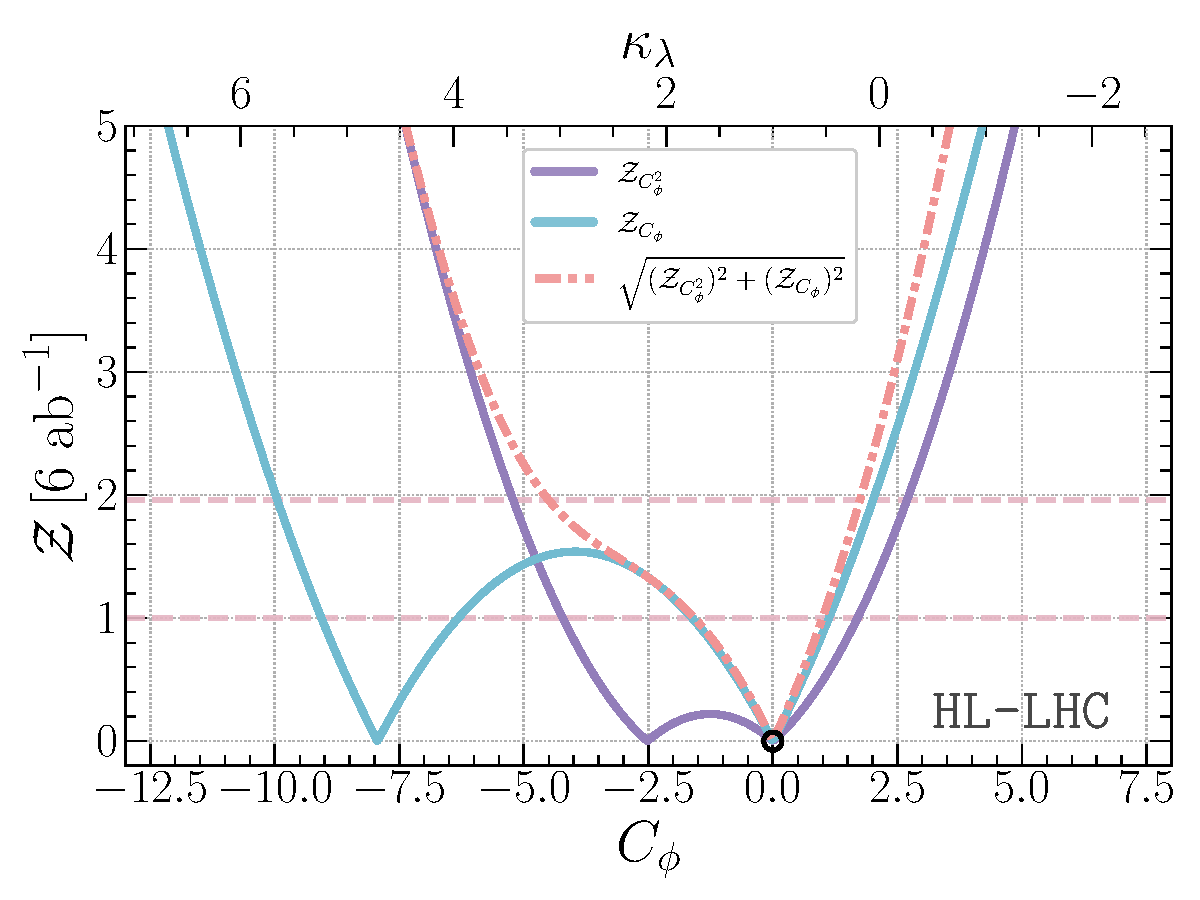
\includegraphics[width=0.47\linewidth]{fig/HL-LHC-sig14.pdf}
	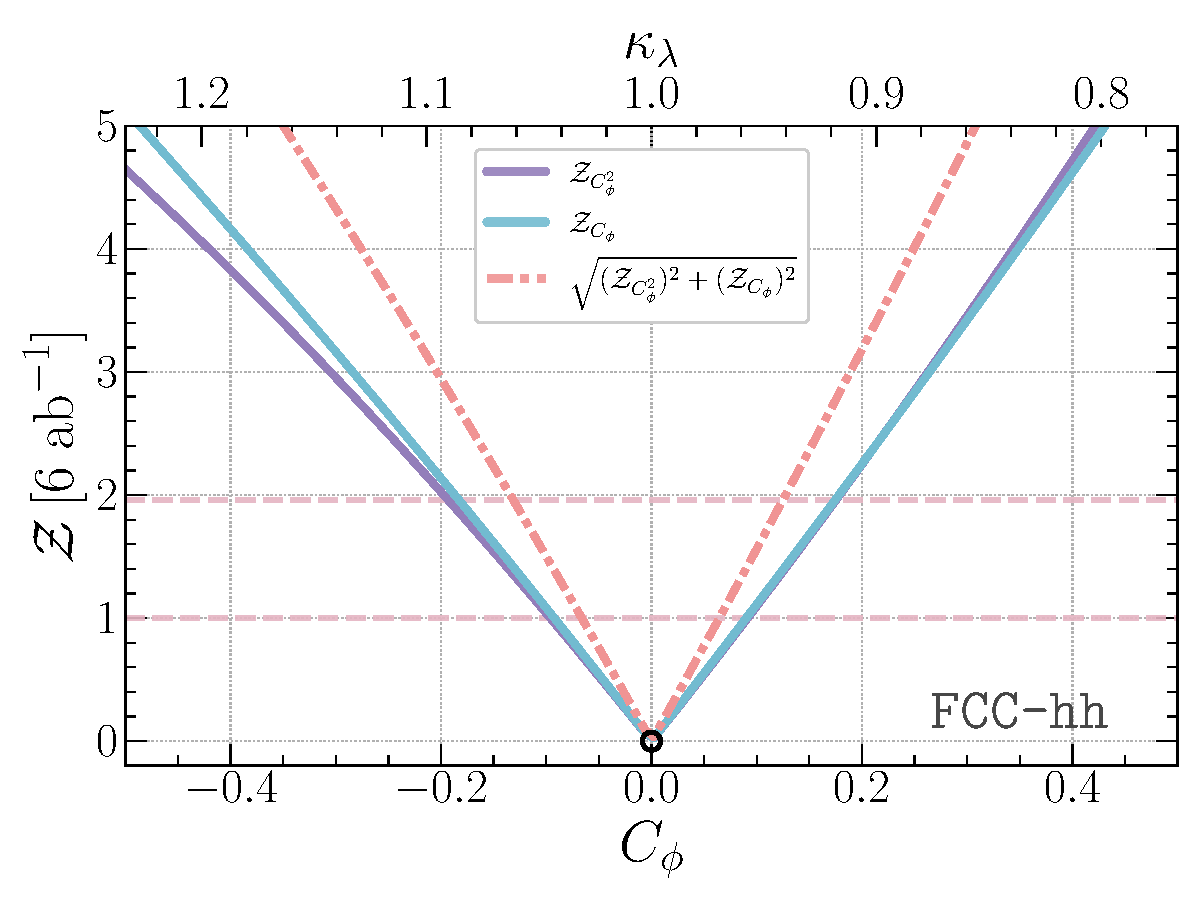
\includegraphics[width=0.47\linewidth]{fig/FCC-hh-sig100.pdf}
	\caption{\it Bounds on $C_\phi$ (or $\kappa_\lambda$) at the HL-LHC (left panel) and the FCC-hh (right panel). The solid blue lines are the constraints coming from the $\hhint$ contribution which scales linearly with the modified coupling and the solid purple line is that from the $\hhtri$ contribution that scales quadratically with the modified coupling. The red dashed line is the combination of the quadratic and linear channel. The horizontal light red dashed lines marks the 68\% and 95\% confidence intervals.}
	\label{fig:constraintkl}
\end{figure}

First, we will show the projections of the limits that can be set on $C_\phi$ (or equivalently, $\kappa_\lambda$) from HL-LHC and FCC-hh. In \autoref{tab:HL-LHC-confusion-CH} we provide the output of the BDT classification for 6 $\iab$ of data collected at HL-LHC and in \autoref{tab:FCC-hh-confusion-CH} we provide the same for 30 $\iab$ of data at FCC-hh. It can be seen from these matrices that while the $\bbaa$ QCD-QED channel is the dominant background, the BDT performs better in separating it from the signal channels than separating $\QQh$. This is due to the kinematic similarities between the signal and the $\QQh$ background.

In \autoref{fig:constraintkl} we present the constraints on $C_\phi$ (or $\kappa_\lambda$) that can be set from HL-LHC in the left panel and FCC-hh in the right panel. The $\hhbox$ topology is not modified by $C_\phi$ and serves as a background to the measurement of $C_\phi$. We separate the constraints from the $\hhtri$, which is quadratic in $C_\phi$ from the $\hhint$ which is linear in $C_\phi$. The combination of the two is given by the red dot-dashed line and is asymmetric around the best fit point, for SM signal injection, $C_\phi=0 \; (\kappa_\lambda=1)$. The projected $1\sigma$ bound on $C_\phi$ is $[-1.57, 1.00]$ at HL-LHC. There is a vast improvement projected for the FCC-hh which is not only due to increased luminosity but also due to the measurement being at a higher energy. The projected $1\sigma$ bound is $C_\phi = [-0.066, 0.064]$. The latter corresponds to a 3\% bound on $\kappa_\lambda$.


%%%%%%%%%%%%%%%%%%%%%%%%%%%%
\subsection{Two and three parameter constraints on \texorpdfstring{$C_\phi$}{CH},  \texorpdfstring{$C_{u\phi}$}{CuH} and \texorpdfstring{$C_{d\phi}$}{CdH}}
\label{sec:multiparam}
%%%%%%%%%%%%%%%%%%%%%%%%%%%%

\begin{table}[]
	\centering
	{\footnotesize
		\begin{tabular}{cccc||ccc}
			\toprule
			Operators &  $C_{u\phi}$&   $C_{d\phi}$&   $C_{\phi}$&    $\kappa_{u}$&   $\kappa_{d}$&   $\kappa_\lambda$\\
			\midrule
			\multicolumn{7}{c}{HL-LHC 14 TeV 6$\inab$}\\
			\midrule
			$\mathcal O_{\phi}$ &--   & --            &[-1.57, 1.00] &--  & -- &[0.53, 1.73]\\
			$\mathcal O_{u\phi}$&[-0.09, 0.10]   & --            &-- &[-477, 431]  & -- &--\\
			$\mathcal O_{d\phi}$&--   & [-0.16, 0.16]            &-- &--  & [-360, 360] &--\\
			$\mathcal O_{u\phi}$ \& $\mathcal O_{\phi}$ &[-0.087, 0.091]  & --            &[-2.42, 0.79] &[-434, 417] & -- &[0.63, 2.13]\\
			$\mathcal O_{d\phi}$ \& $\mathcal O_{\phi}$ & --             &[-0.17, 0.17]  &[-2.73, 0.77]& -- &[-381, 379] &[0.63, 2.27]\\
			$\mathcal O_{u\phi}$ \& $\mathcal O_{d\phi}$&[-0.065, 0.069]&[-0.12, 0.12]& --            &[-331, 312] &[-268, 272] & -- \\
			All                                   &[-0.077, 0.084]&[-0.160, 0.162]& [-2.77, 0.43]&[-400, 369] &[-362, 359] & [0.79, 2.30] \\
			\midrule
			\midrule
			\multicolumn{7}{c}{FCC-hh 100 TeV 30$\inab$}\\
			\midrule
			$\mathcal O_{\phi}$ &--   & --            &[-0.066, 0.064] &--  & -- &[0.97, 1.03]\\
			$\mathcal O_{u\phi}$&[-0.012, 0.011]   & --            &-- &[-57.8, 54.7]  & -- &--\\
			$\mathcal O_{d\phi}$&--   & [-0.012, 0.011]            &-- &--  & [-26.3, 28.4] &--\\
			$\mathcal O_{u\phi}$ \& $\mathcal O_{\phi}$ &[-0.010, 0.011]  & --            &[-0.091, 0.042] &[-52, 49] & -- &[0.98, 1.04]\\
			$\mathcal O_{d\phi}$ \& $\mathcal O_{\phi}$ & --             &[-0.010, 0.012]  &[-0.092, 0.041]& -- &[-24, 26] &[0.98, 1.04]\\
			$\mathcal O_{u\phi}$ \& $\mathcal O_{d\phi}$&[-0.008, 0.009]&[-0.008, 0.009]& --            &[-42, 39] &[-19,19] & -- \\
			All                                   &[-0.009, 0.010]&[-0.009, 0.010]& [-0.105 0.023]&[-47, 44] &[-21, 21] & [0.99, 1.05] \\
			\bottomrule
		\end{tabular}
	}
	\caption{\it The 1$\sigma$ bounds on $C_{u\phi}$, $C_{d\phi}$ and $C_\phi$ from one-, two- and three-parameter fits for HL-LHC with 6$\inab$ of data and FCC-hh with 30$\inab$ of data. The corresponding bounds on the rescaling of the effective couplings, $\kappa_u$, $\kappa_d$ and $\kappa_\lambda$ are presented on the right side of the table.}
	\label{tab:twoparambounds}
\end{table}

The primary focus of this work is to move beyond just looking at constraints on $C_\phi$ from di-Higgs production and to shed light on how simultaneous modifications of the light-quark Yukawa couplings due to non-zero contributions from $C_{u\phi}$ and $C_{d\phi}$ can change the constraints on $C_\phi$. The modifications of the light-quark Yukawa couplings manifest themselves in two different ways. Firstly, non-zero $C_{u\phi}$ and $C_{d\phi}$ open up the $q\bar q \to hh$ production mode through a point interaction (see \autoref{fig:qqa}) thus changing the production cross-section of the di-Higgs channel. This increase in the production cross-section sets the tightest constraints on $C_{u\phi}$ and $C_{d\phi}$ from di-Higgs production. Secondly, the modification of the light-quark Yukawa couplings also modify the branching fraction of $h\to\gamma\gamma$ and the width of the Higgs. The latter modifies the channels that are also sensitive to $C_\phi$, thus modifying the constraints that can be set on $C_\phi$ from future measurements. Such constraints are the subdominant ones on $C_{u\phi}$ and $C_{d\phi}$ but they are necessary for a holistic picture.

In the two parameter fits, we consider three possible scenarios. Firstly, one can assume that the trilinear Higgs coupling is not modified and only the light-quark Yukawa couplings are. Two other possibilities are the simultaneous modification of the $C_\phi$ and one of $C_{u\phi}$ and $C_{d\phi}$. These are the three constraints that we show in \autoref{fig:constraint2d}. 
%\rg{why are the bounds on $C_{d\phi}$ and $C_{u\phi}$ non symmetric once you have them together with $C_\phi$? Is this purely numeric?} 
As before, the constraints have been obtained by training the BDT to separate the relevant signal channels from the background, the signal used being the one corresponding to the pair of Wilson coefficients that we intend to constrain. The confusion matrices for all the three cases can be found in the \texttt{Github} repository for this analysis. The left panels of \autoref{fig:constraint2d} show the projected constraints for HL-LHC and right panels for the FCC-hh.

Comparing with the constraints on $C_\phi$ given in \autoref{sec:CH} and~\autoref{fig:constraintkl}, it can be seen from the top and middle left panels of~\autoref{fig:constraint2d} that, indeed, the constraints on $C_\phi$ are diluted when the light-quark Yukawa couplings are allowed to vary. This effect is somewhat more prominent for $C_{d\phi}$ than for $C_{u\phi}$ and stems from the fact that away from $C_{u\phi,d\phi} = 0$ larger negative values of $C_\phi$ are allowed by the crescent shaped curves in~\autoref{fig:constraint2d}. For $C_{d\phi}$ vs.~$C_\phi$ the 3$\sigma$ region is unbounded in the domain $|C_{d\phi}| \gtrsim 0.6$. The bounds on $C_{u\phi}$ and $C_{d\phi}$ from the fit with two-parameters including $C_\phi$ remain the same as the bounds on these Wilson coefficient from the single parameter $C_{u\phi,d\phi}$ fits. We summarize the results in~\autoref{tab:twoparambounds}. 

It should be noted that the two-parameter fit for $C_{u\phi}$ and $C_{d\phi}$ provide a stronger bound on the two parameters than the fit done individually. While this might be a bit counter-intuitive considering constraints from fits tend to deteriorate with the increasing number of parameters, we found that is not the case here. The reason is that the two-parameter fit is performed with the predictions made by the BDT trained with simulated events for both $\uuA$ and $\ddA$. Between these two channels, each form the background for the other when separating them through a confusion matrix. Since the training also give the proportion of mistagged events, both the signal and the backgrounds are modified by the Wilson coefficients leading to a greater deformation of the likelihood in a favourable direction such that the constraints on the Wilson coefficients in the two-parameter fit is better than for the case in which they were separated from other $\bbaa$ backgrounds individually.
\begin{figure}[t!]
	\centering
	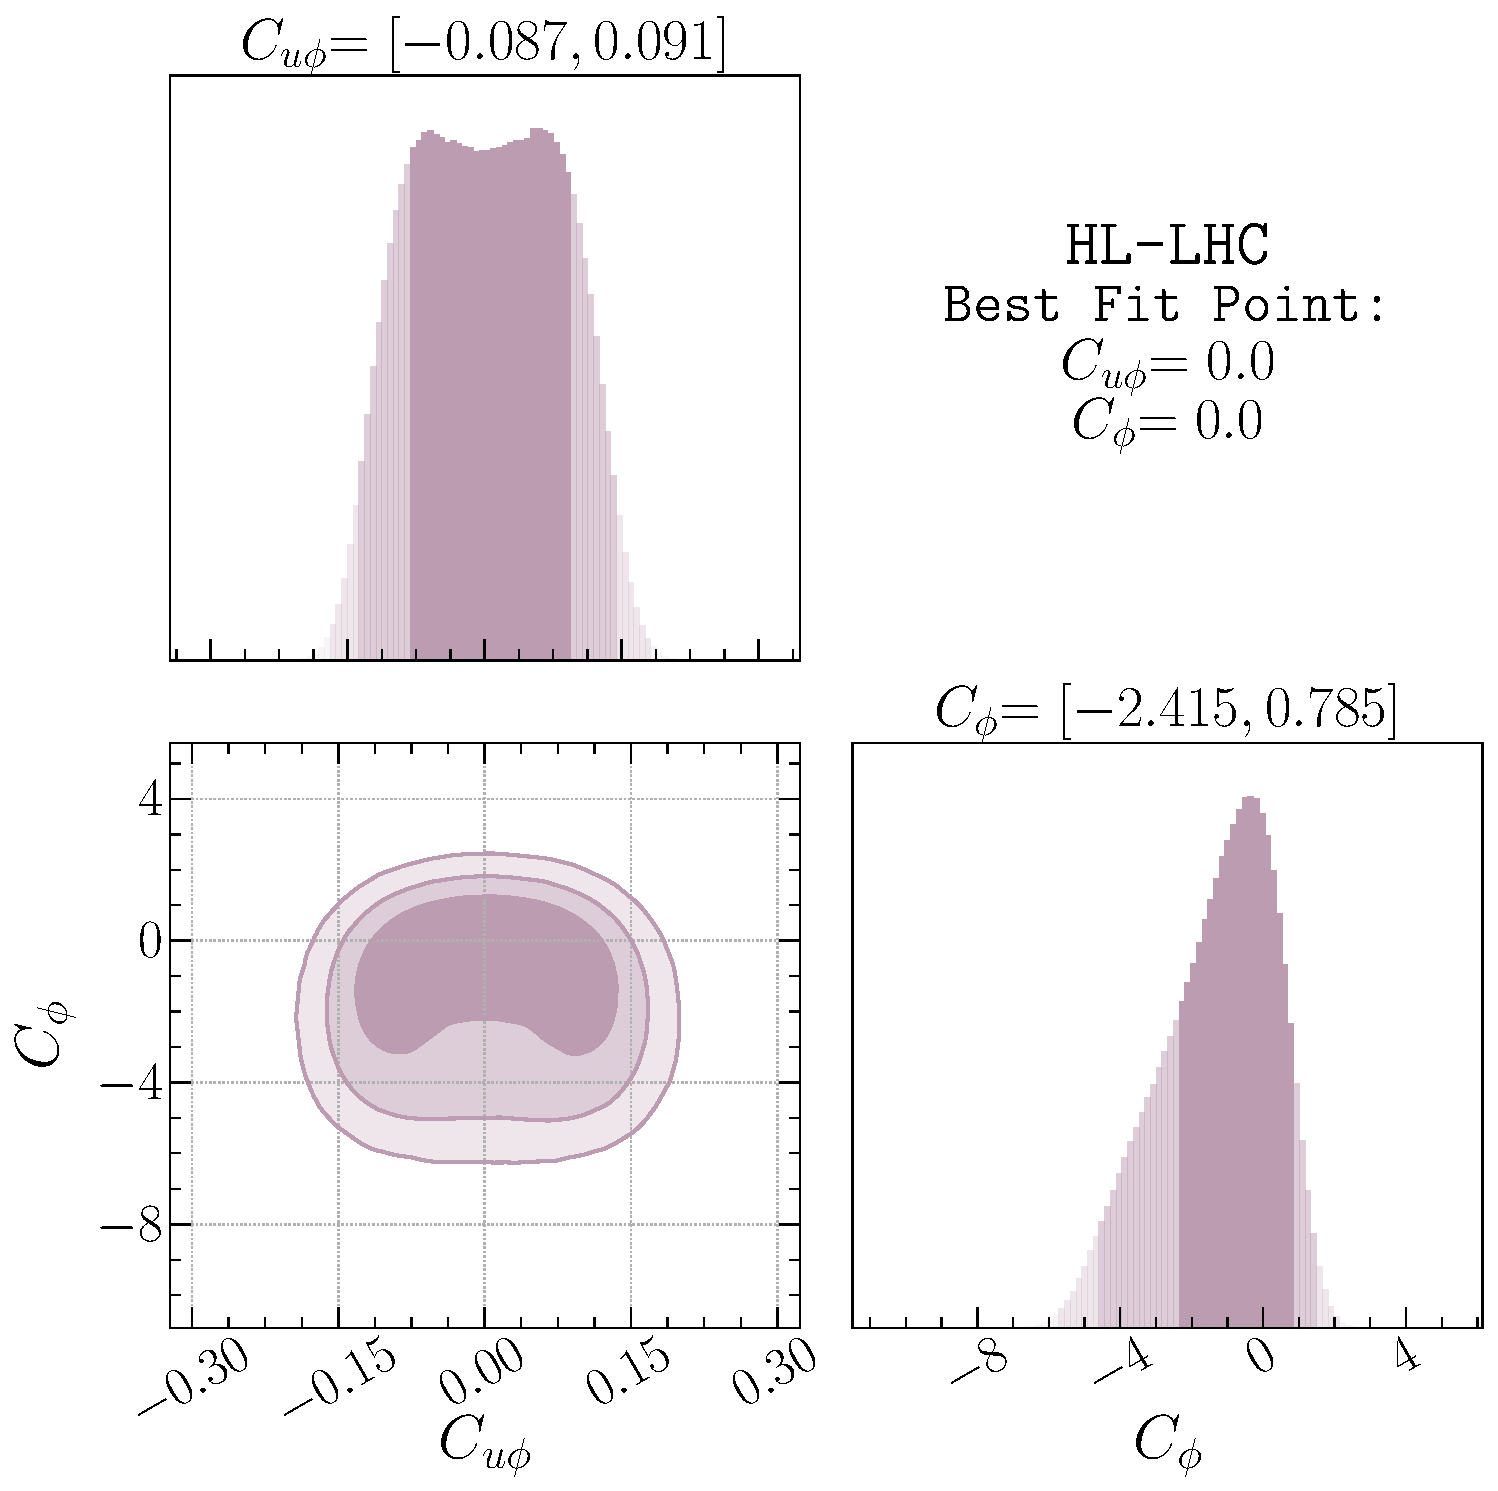
\includegraphics[width=0.47\linewidth]{fig/kappa_u-kappa_l-HL-LHC.pdf}
	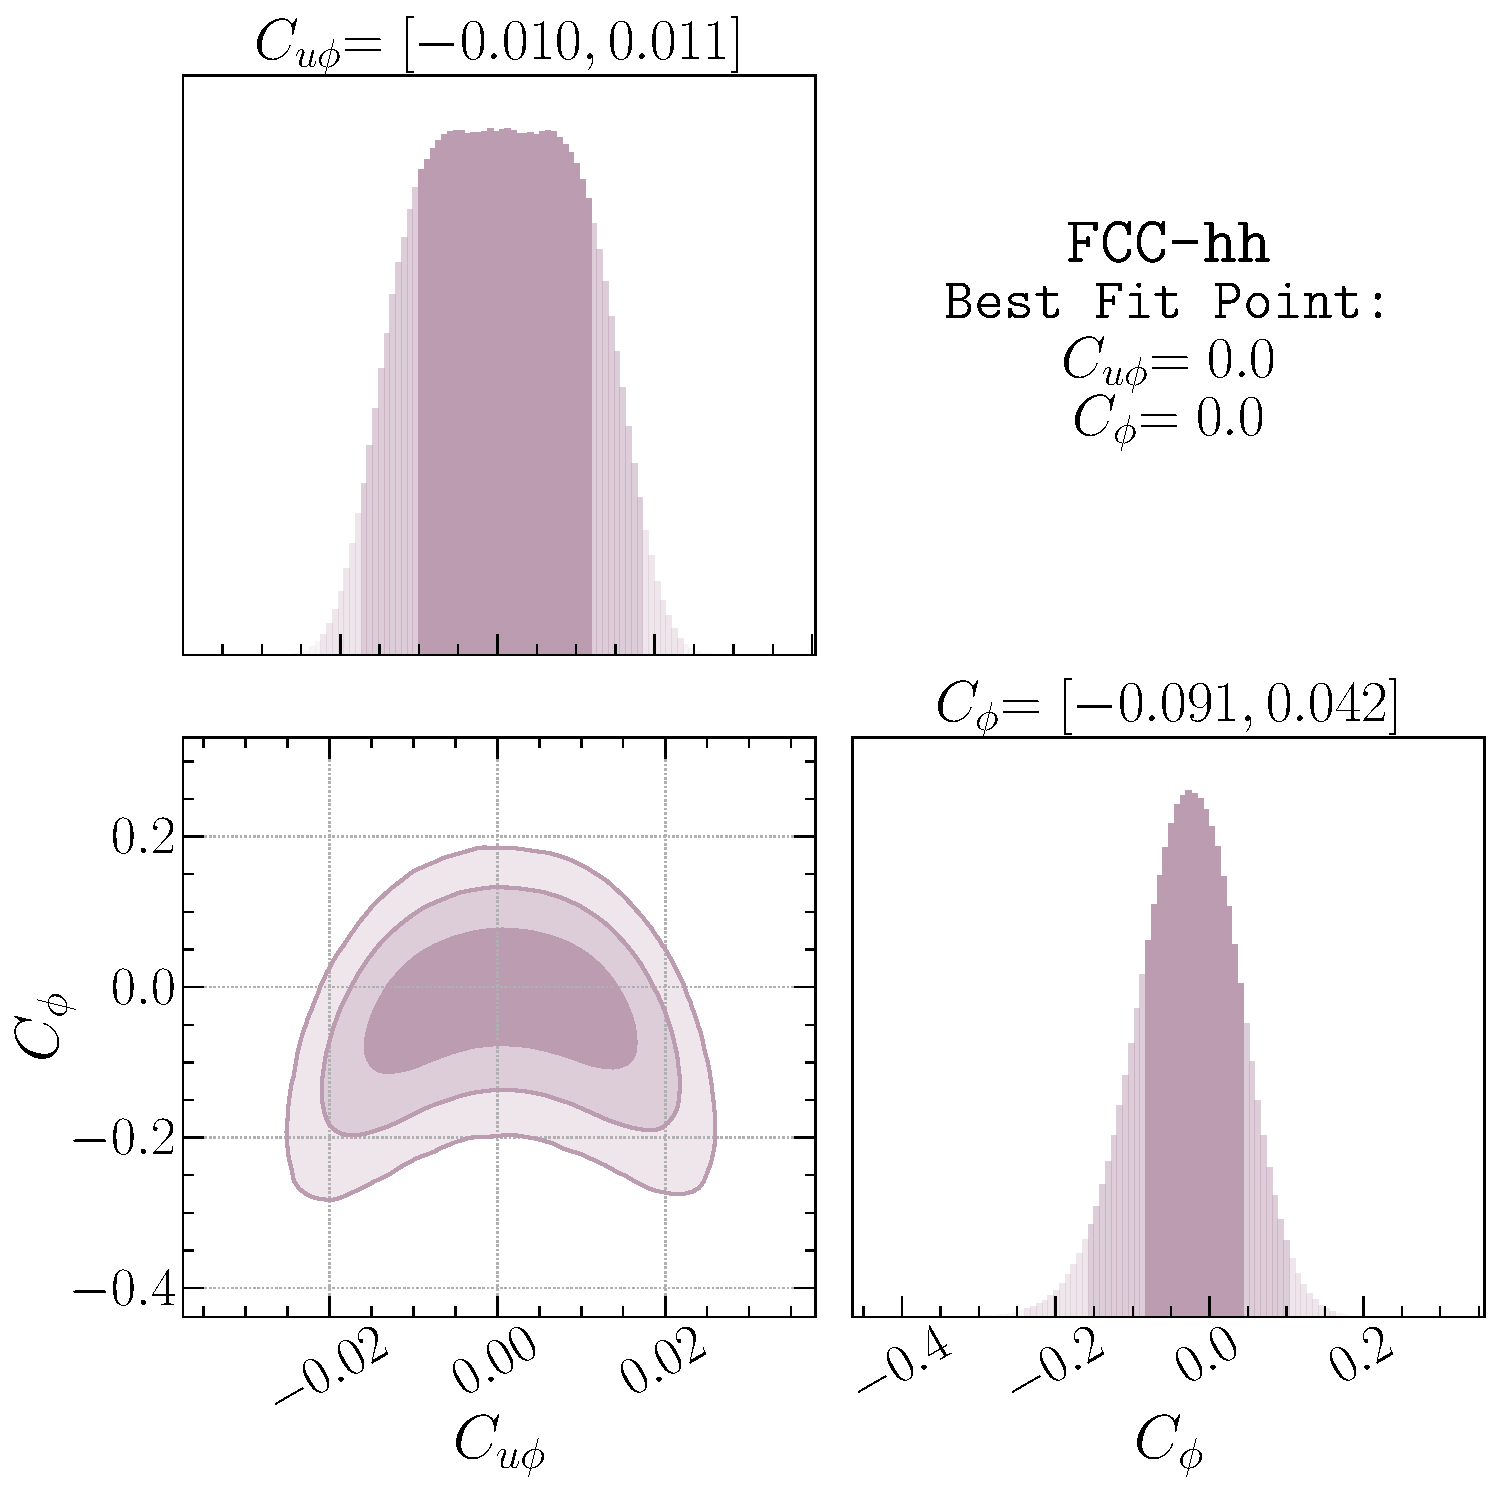
\includegraphics[width=0.47\linewidth]{fig/kappa_u-kappa_l-FCC-hh.pdf}
	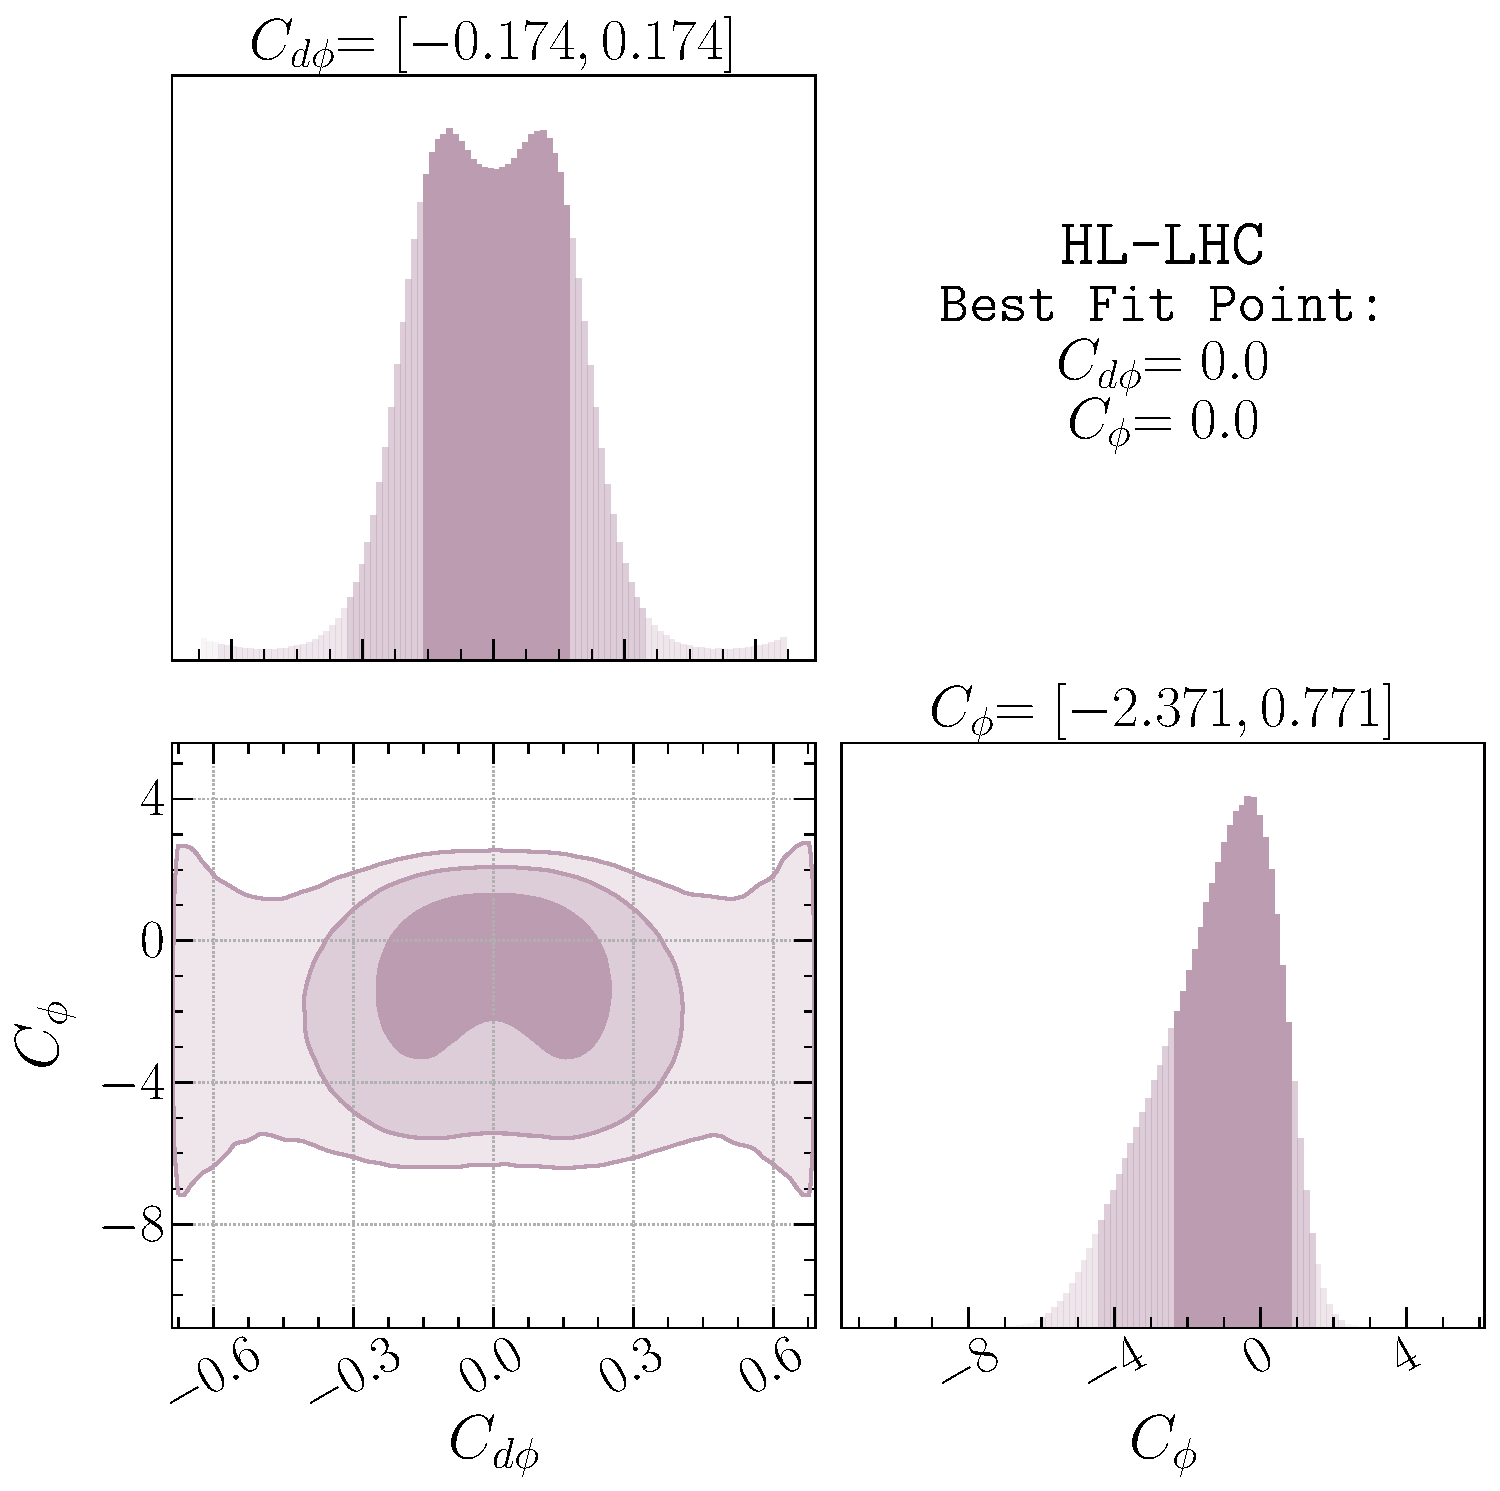
\includegraphics[width=0.47\linewidth]{fig/kappa_d-kappa_l-HL-LHC.pdf}
	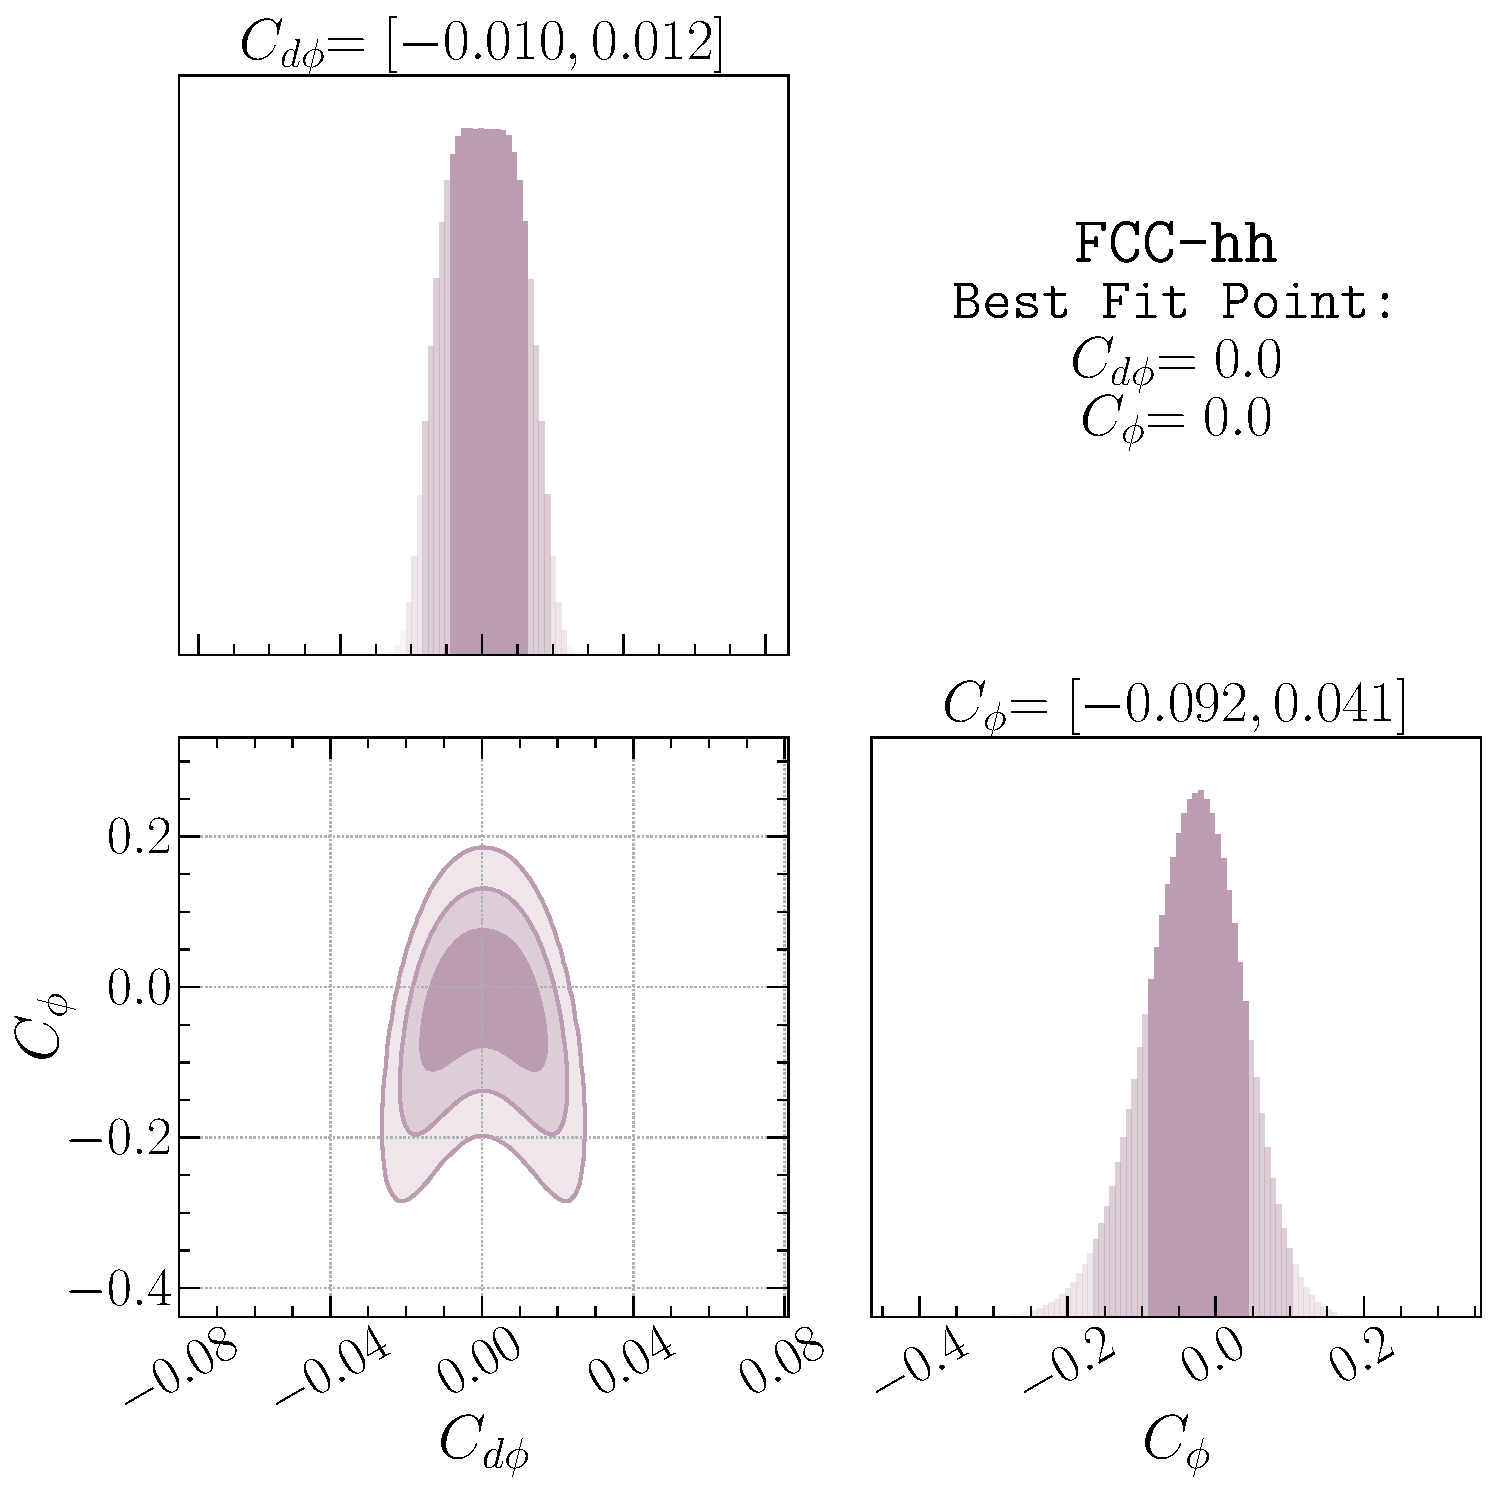
\includegraphics[width=0.47\linewidth]{fig/kappa_d-kappa_l-FCC-hh.pdf}
	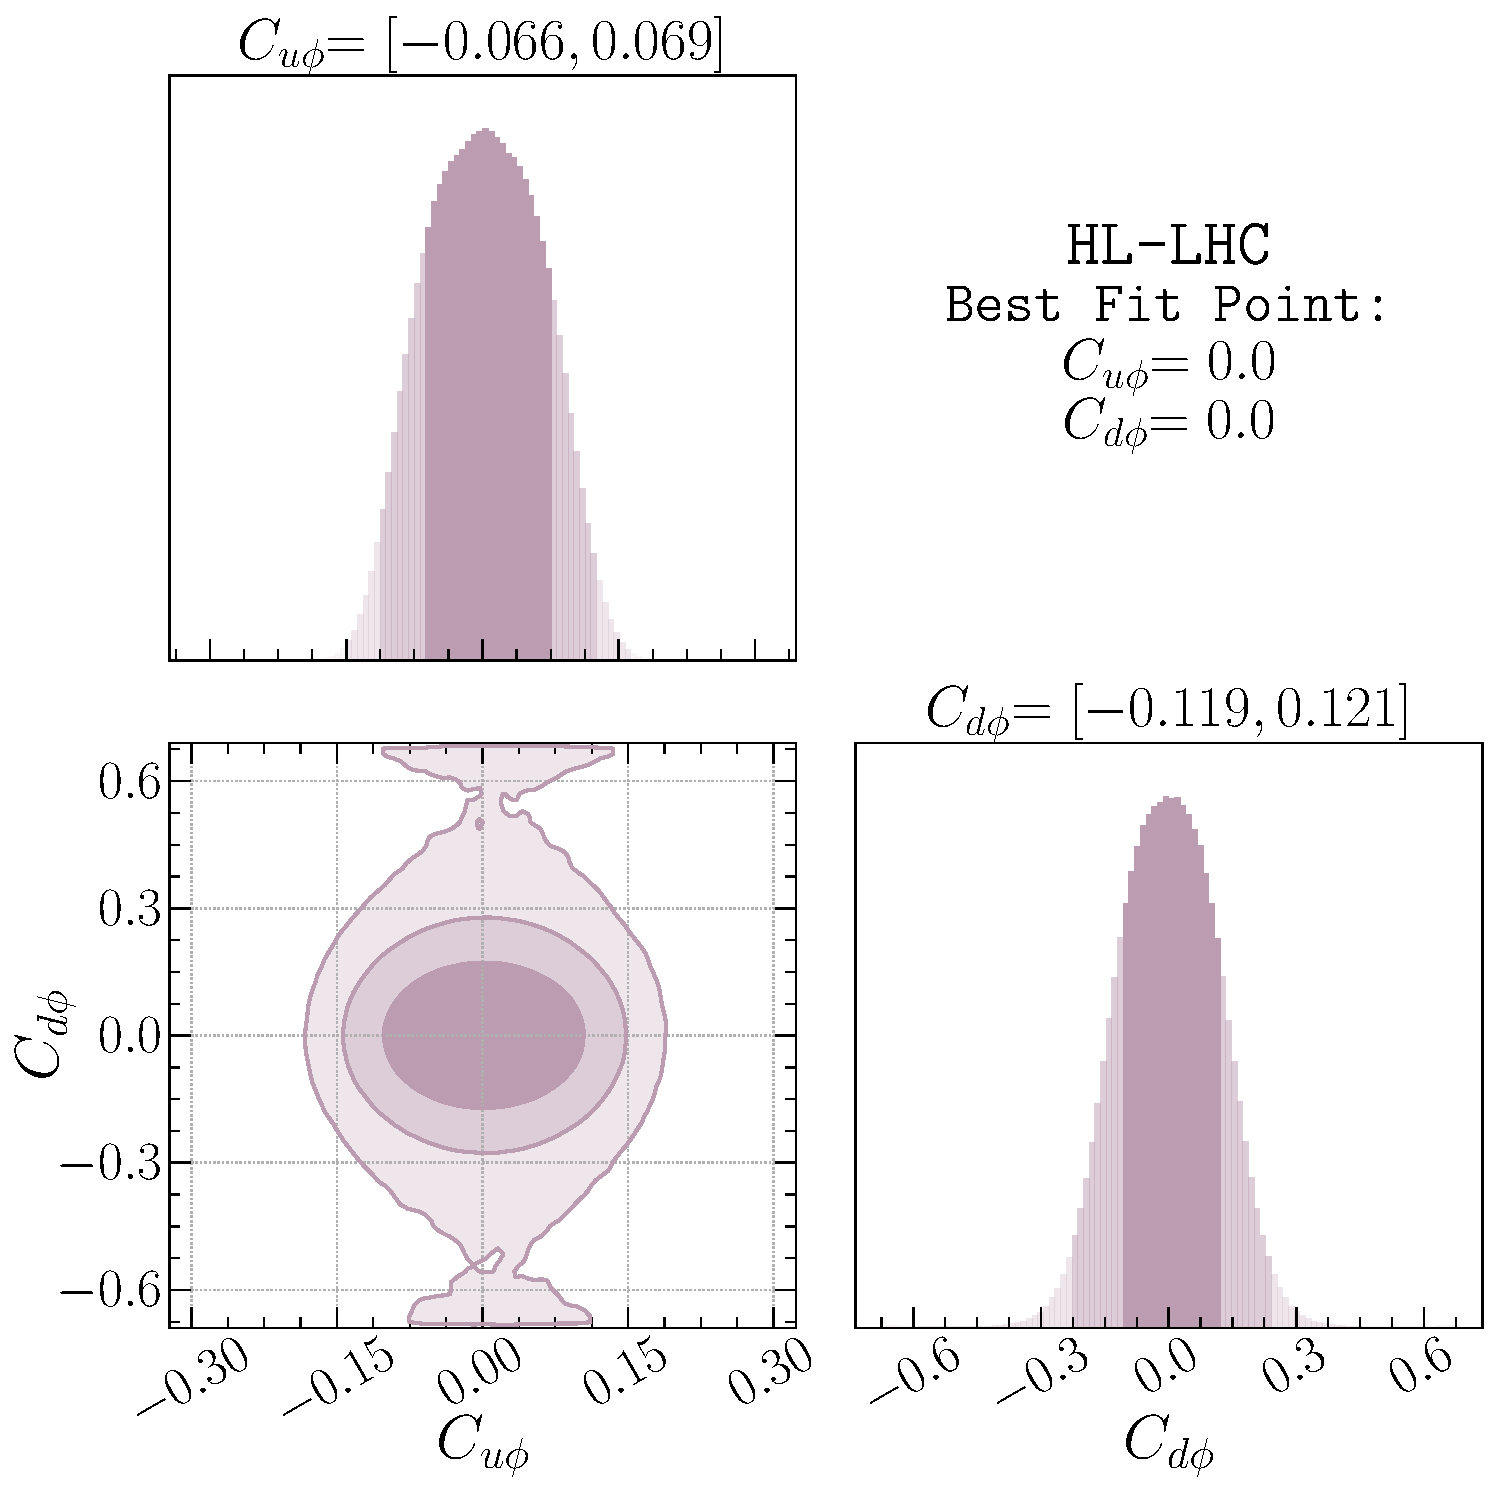
\includegraphics[width=0.47\linewidth]{fig/kappa_u-kappa_d-HL-LHC.pdf}
	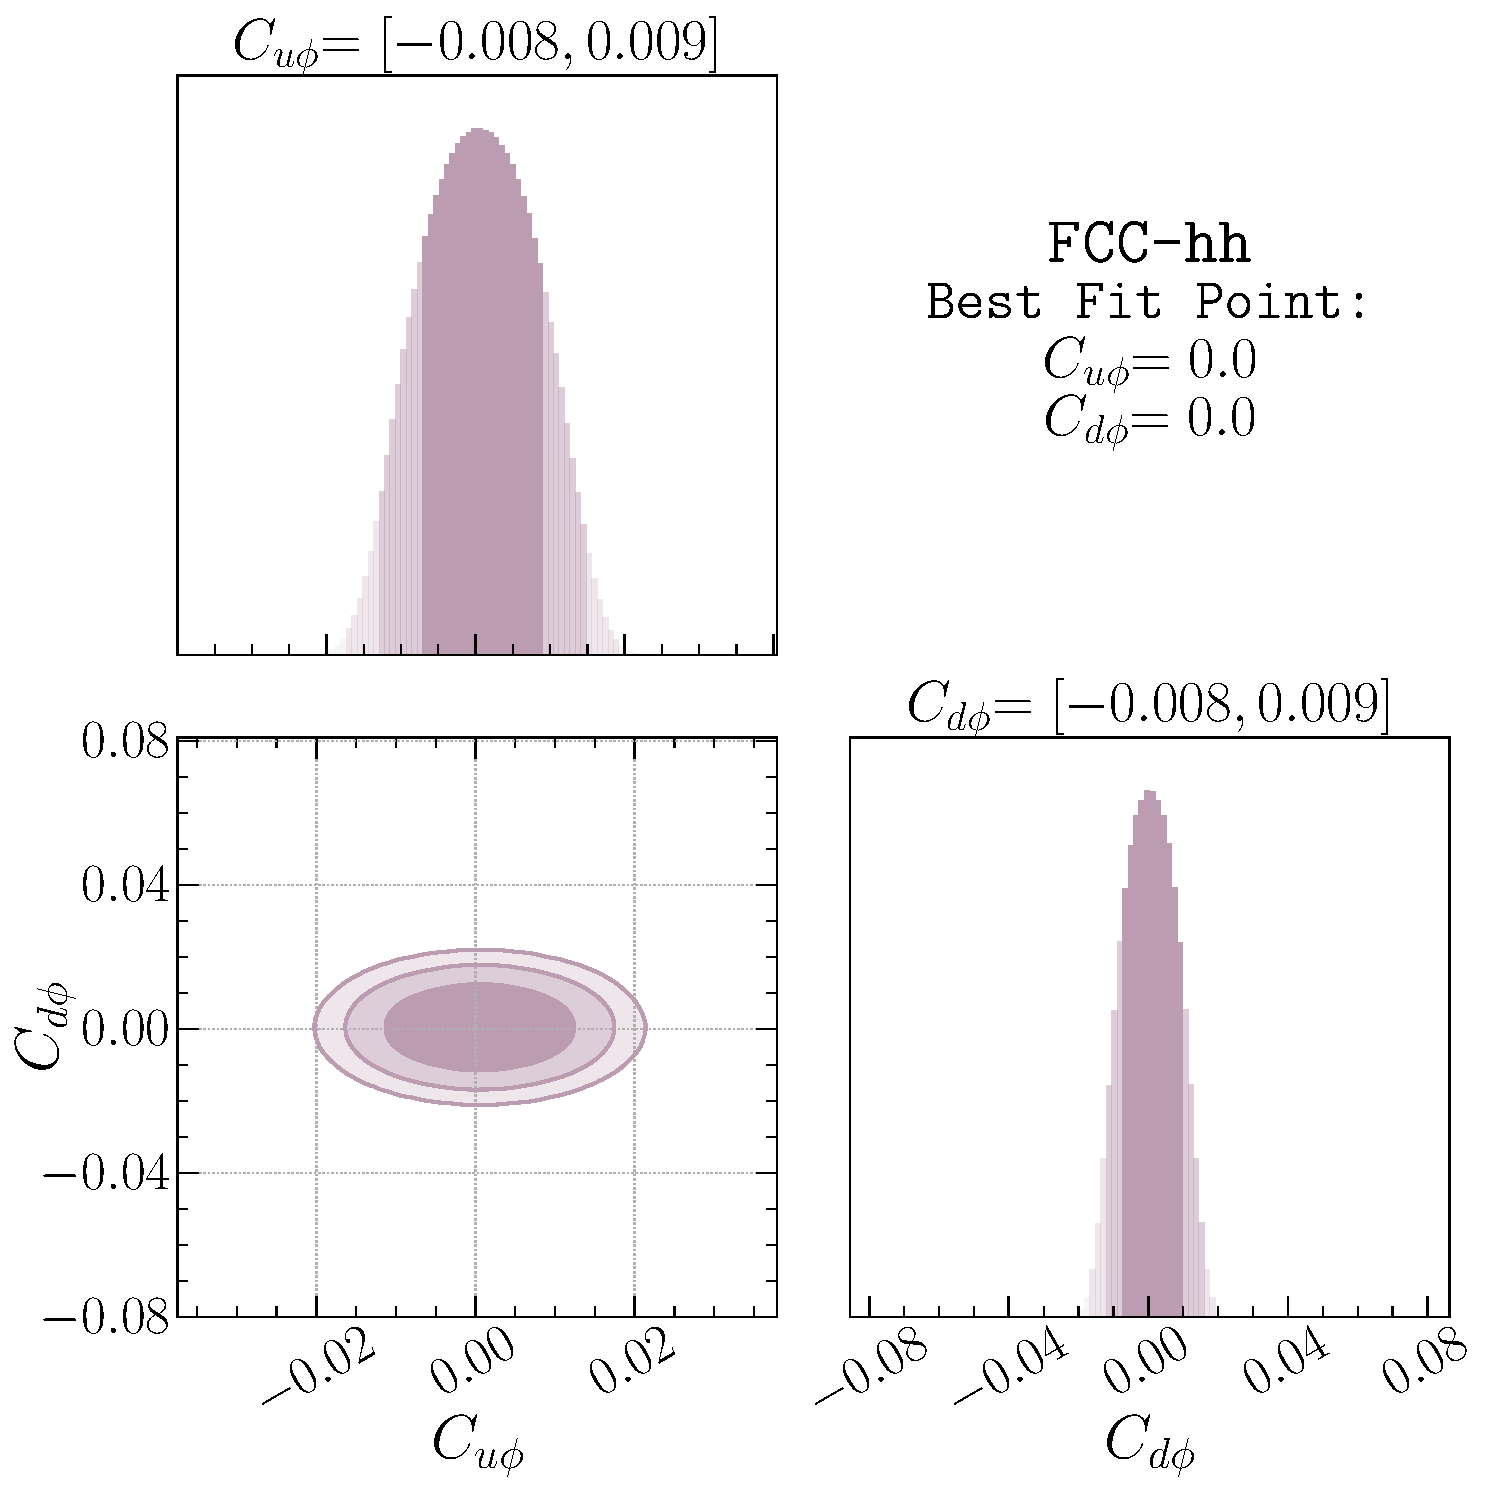
\includegraphics[width=0.47\linewidth]{fig/kappa_u-kappa_d-FCC-hh.pdf}
	\caption{\it Constraints on pairs of Wilson coefficients for $C_\phi$, $C_{u\phi}$ and $C_{d\phi}$, The panels of the left are for HL-LHC with 6 $\iab$ of luminosity and the ones on the right are for FCC-hh with 30 $\iab$ of luminosity.}
	\label{fig:constraint2d}
\end{figure}
\FloatBarrier

\begin{figure}[t!]
	\centering
	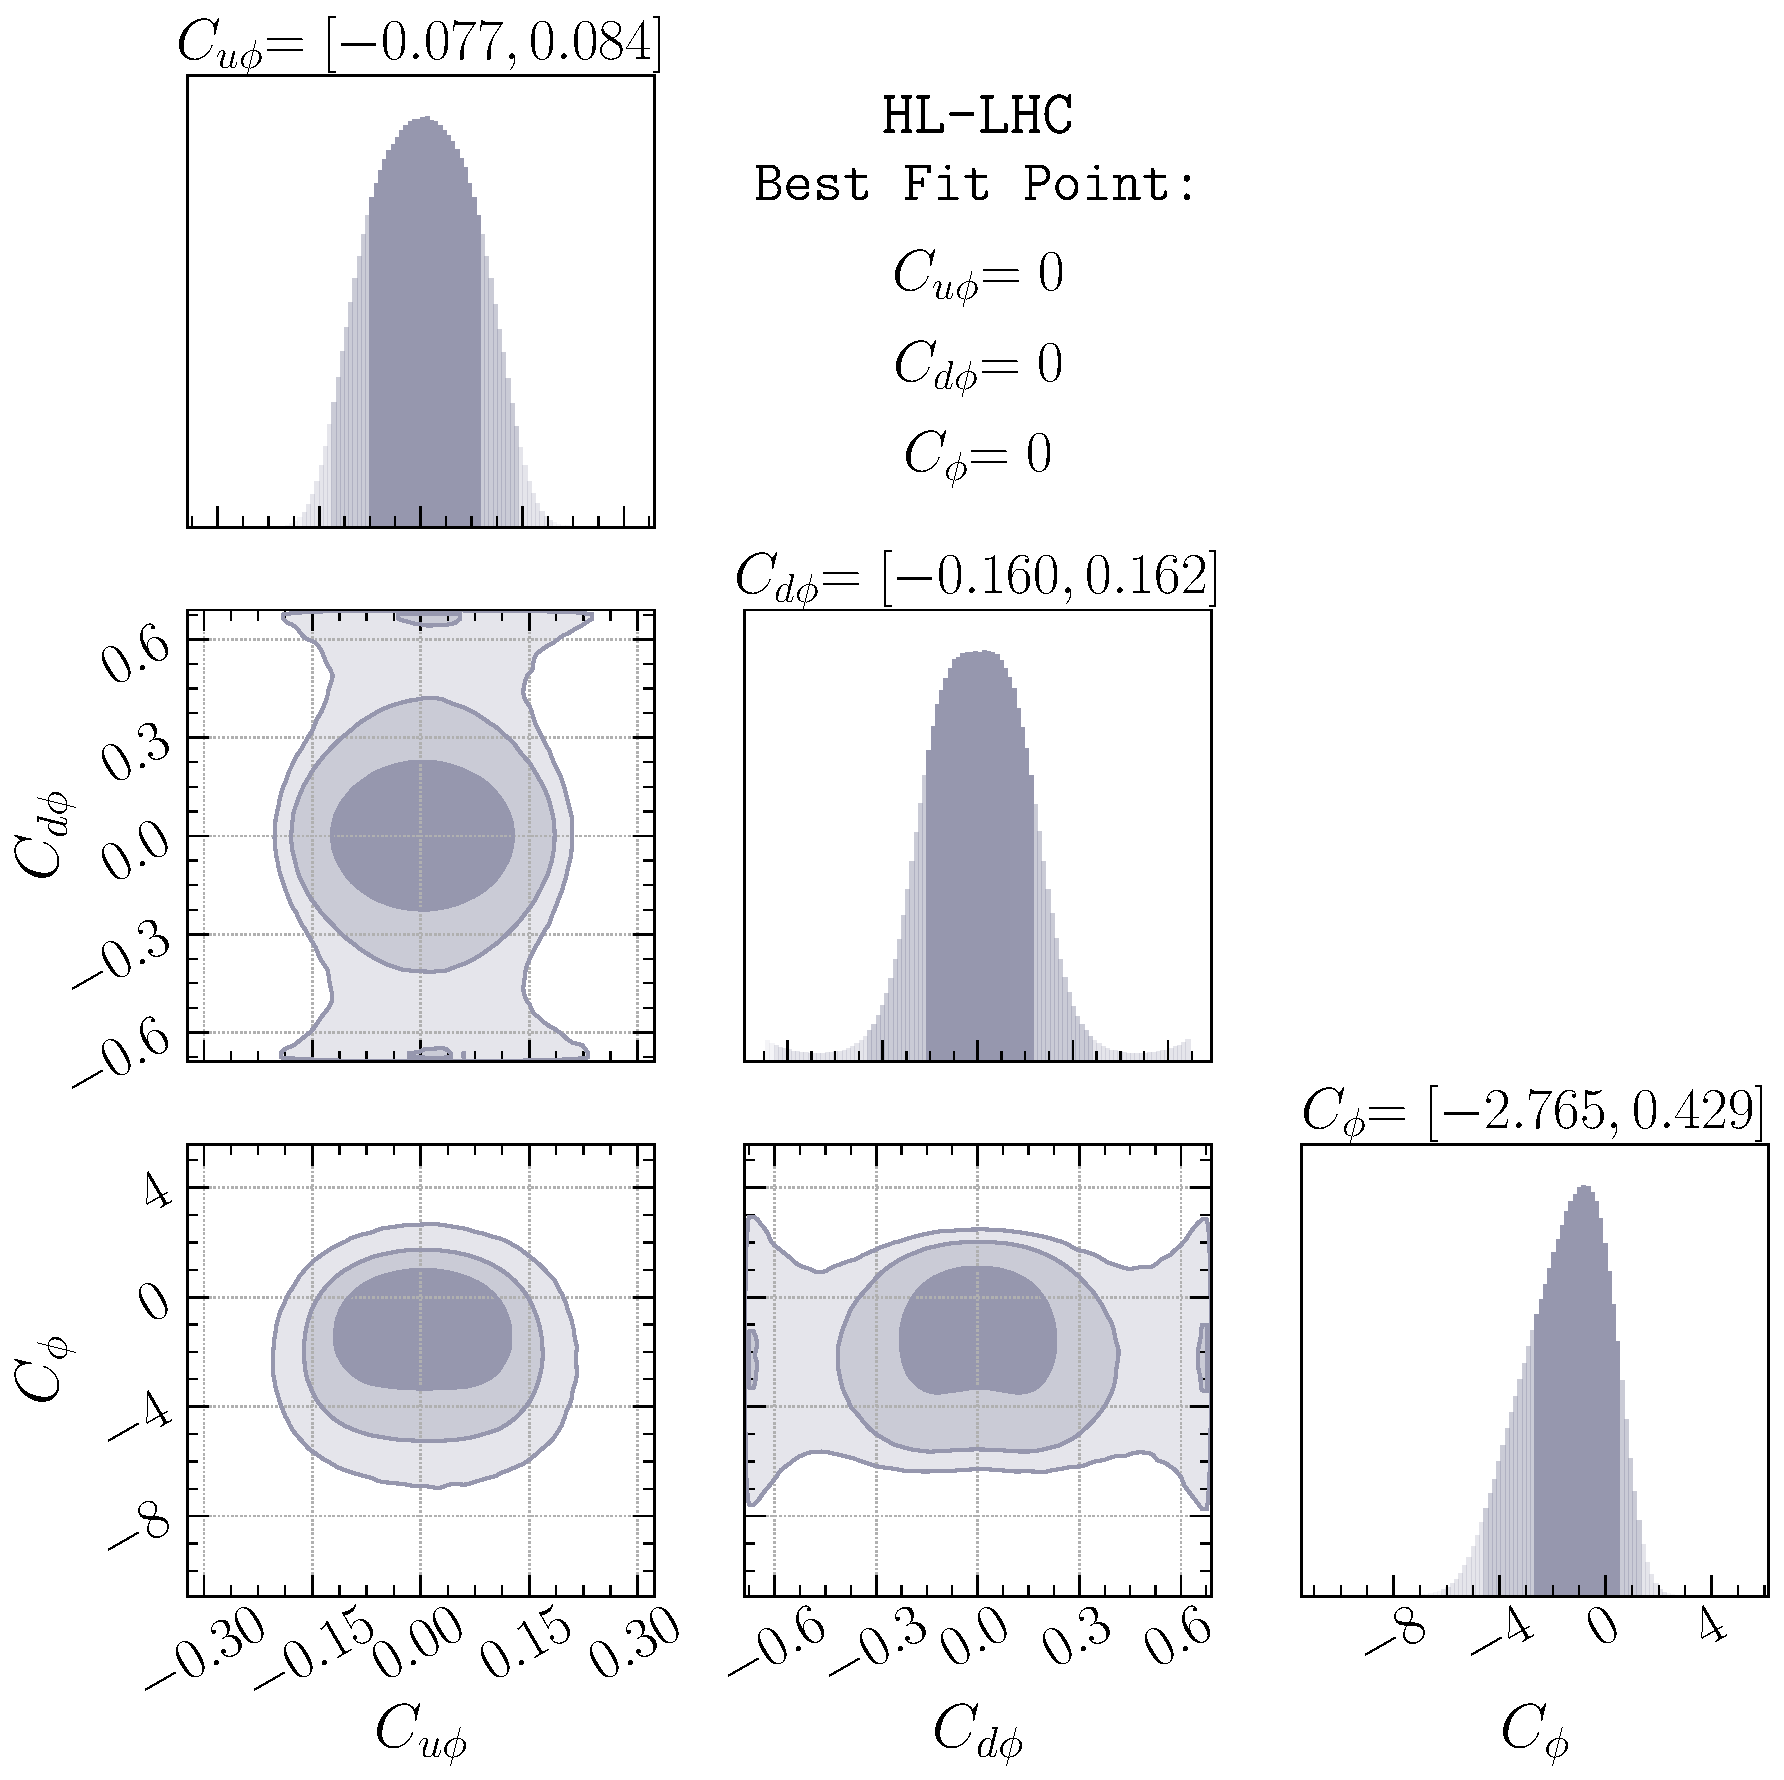
\includegraphics[width =0.47\linewidth]{fig/kappa_u-kappa_d-kappa_l-HL-LHC.pdf}
	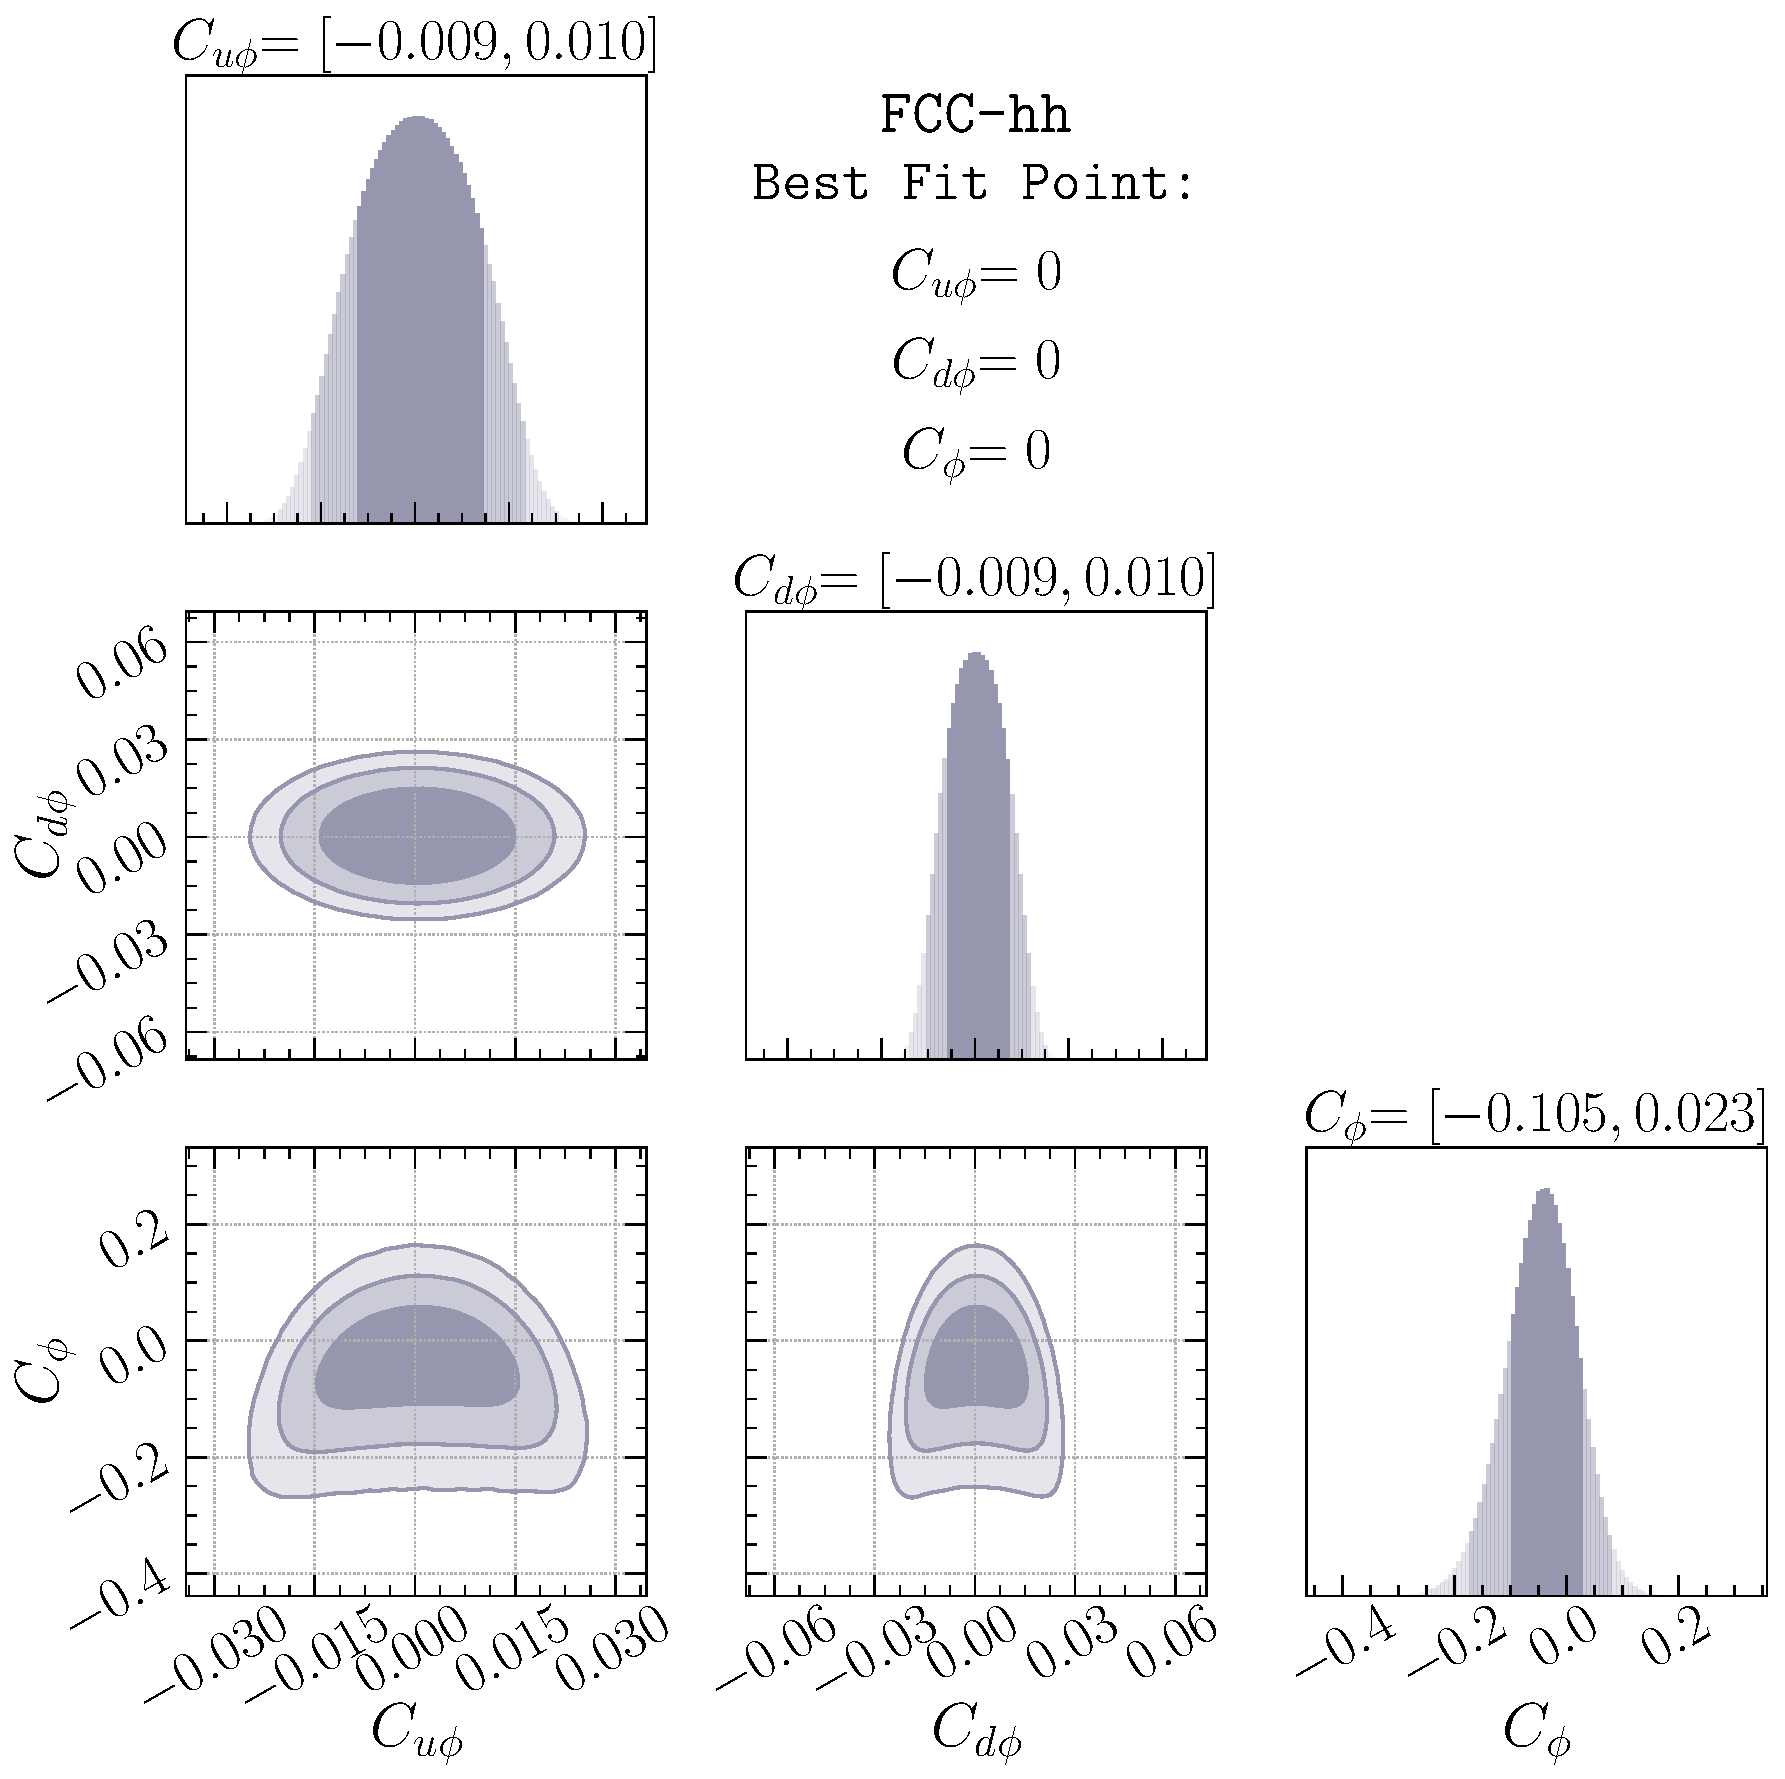
\includegraphics[width =0.47\linewidth]{fig/kappa_u-kappa_d-kappa_l-FCC-hh.pdf}
	\caption{\it Three parameter fits with $C_{u\phi}$, $C_{d\phi}$ and $C_\phi$, 6$\inab$ of luminosity at 14 TeV for HL-LHC (left panel) and 30$\inab$ of luminosity at 100 TeV for FCC-hh (right panel).}
	\label{fig:constraint3d}
\end{figure}

Finally, we perform a combined three-parameter fit including $C_{u\phi}$, $C_{d\phi}$ and $C_\phi$, with the results shown in~\autoref{fig:constraint3d}. For the same reason as explained before, the bounds on $C_{u\phi}$ and $C_{d\phi}$ are somewhat better than the two-parameter fits of these operators individually with $C_\phi$. The HL-LHC and FCC-hh projected bounds on $C_\phi$ remain nearly the same as those from the corresponding two-parameter fits. In~\autoref{tab:twoparambounds} we also provide the bounds on $\kappa_u$, $\kappa_d$ and $\kappa_\lambda$ for comparison.

%%%%%%%%%%%%%%%%%%%%%%%%%%%%
\subsection{Interpretation of Shapley values}
\label{sec:multiparam}
%%%%%%%%%%%%%%%%%%%%%%%%%%%%

Finally, we want to demonstrate the interpretability of the machine learning framework we use and discuss the physics that allows for the separation of the signal channels from the background channels. The advantage of using an interpretable multivariate framework is that one can easily understand which of the kinematic variables are important for orchestrating this separation in a manner that significantly improves upon a cut-and-count analysis. As described previously, we use a measure derived from Shapley values, $\overline{|S_v|}$, to understand the importance of each kinematic variable and, henceforth, understand the differences in kinematic shapes that seperate the signal from the background.

To give a feeling of what the values of $S_v$ mean, let us examine a single event. Assuming we have trained the BDT with $n$ kinematic variables, each event with $n\times m$ Shapley values associated with it, $m$ being the number of channels (signal and background channels). For a particular channel, $j$ and kinematic variable, $i$, $S_v$ can be positive or negative. A positive value implies that it is more likely  that the event belongs to channel $j$ according to the value of the kinematic variable $i$. Conversely, a negative value implies that the event is less likely to belong to channel $j$ given the value of the kinematic variable $i$. So regardless of whether $S_v$ is positive or negative it helps in the sorting of events into various channels. Hence, $\overline{|S_v|}$ for a particular variable represents the strength of the variable to distinguish between channels. When summed over all channels this gives an overall picture of how good a discriminant a kinematic variable is for the processes involved. This is what is shown in \autoref{fig:shap} which we will now elaborate upon.

To begin with, we take a look at the $\overline{|S_v|}$ computed for the five channel analysis performed for separating $\hhtri$ and $\hhint$ channels from $\hhbox$, $\QQh$ and $\bbaa$ QCD-QED background. In \autoref{fig:shap} we see the hierarchy plots for HL-LHC (top left panel) and FCC-hh (top right panel) generated from the predictions made by the BDT for this five channel analysis. For both the colliders, $H_T$ is the most important variable that is bringing about separation of the $\hhtri$ and $\hhint$ channels from the dominating $\bbaa$ QCD-QED background. The second most important variable is $m_{\gamma\gamma}$. The importance of $m_{\gamma\gamma}$ accentuates the separation of the background by a greater degree at FCC-hh than at HL-LHC.

\begin{figure}[t!]
	\centering
	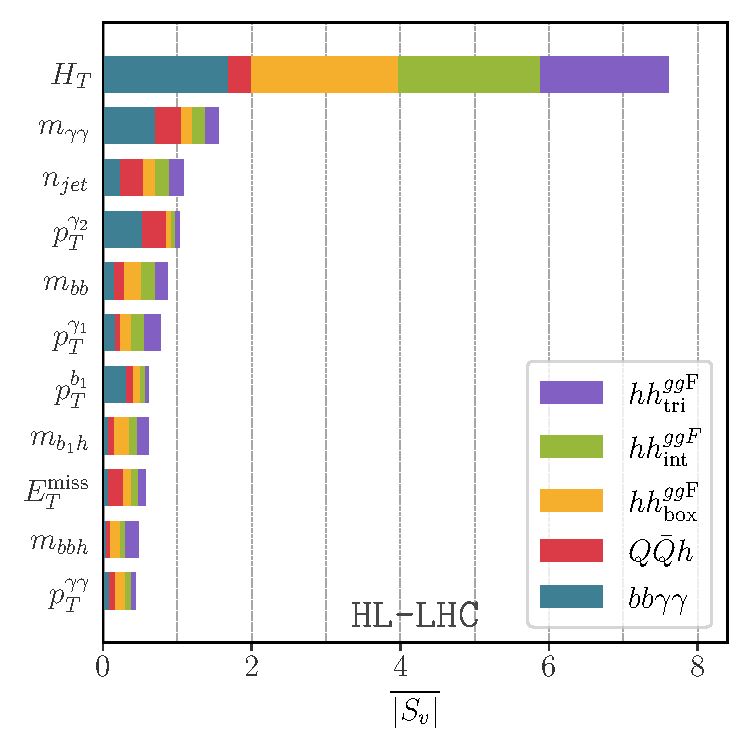
\includegraphics[width=0.45\linewidth]{fig/HL-LHC-shap-bbxaa-bbh-tth-hhsm.pdf}
	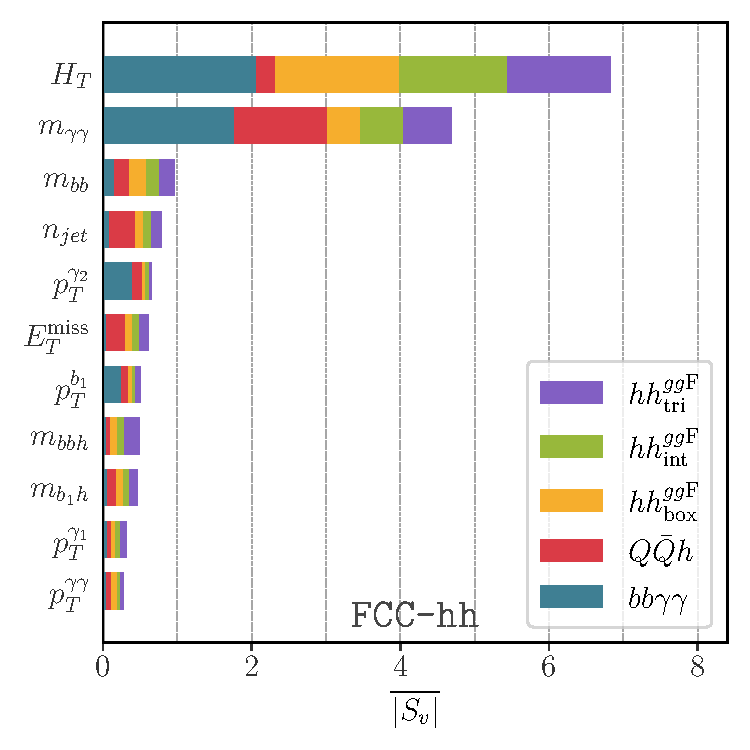
\includegraphics[width=0.45\linewidth]{fig/FCC-hh-shap-bbxaa-bbh-tth-hhsm.pdf}
	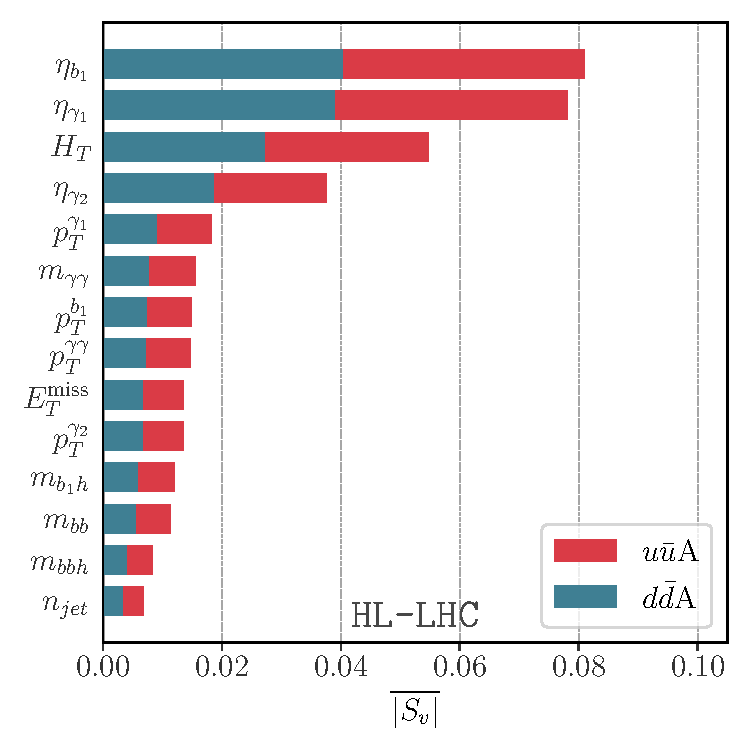
\includegraphics[width=0.45\linewidth]{fig/HL-LHC-shap-ku-kd.pdf}
	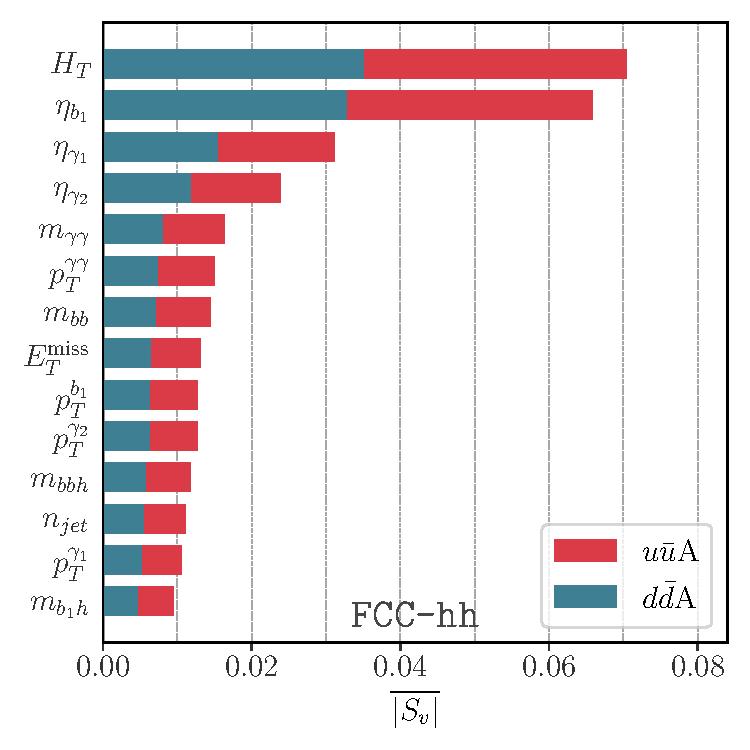
\includegraphics[width=0.45\linewidth]{fig/FCC-hh-shap-ku-kd.pdf}
	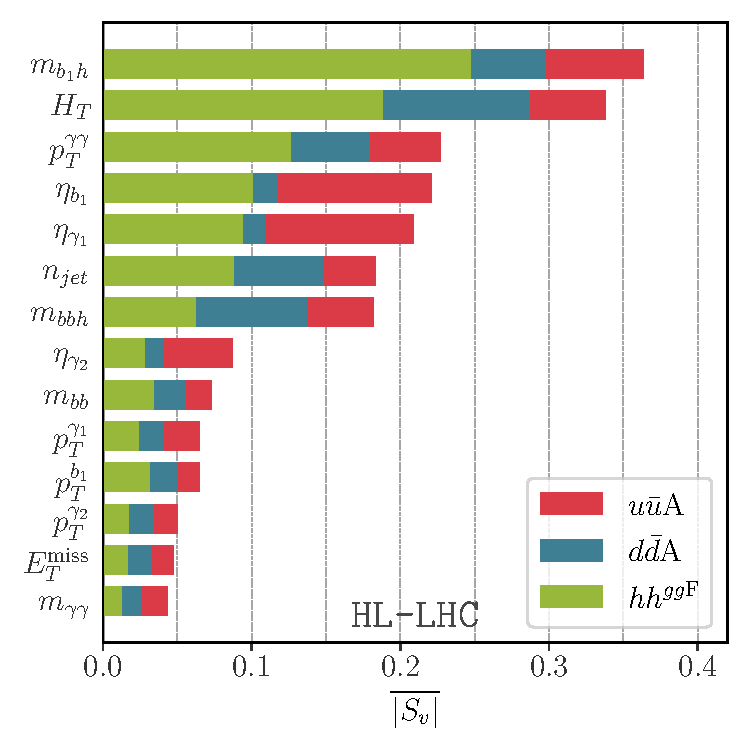
\includegraphics[width=0.45\linewidth]{fig/HL-LHC-shap-ku-kd-hhsm.pdf}
	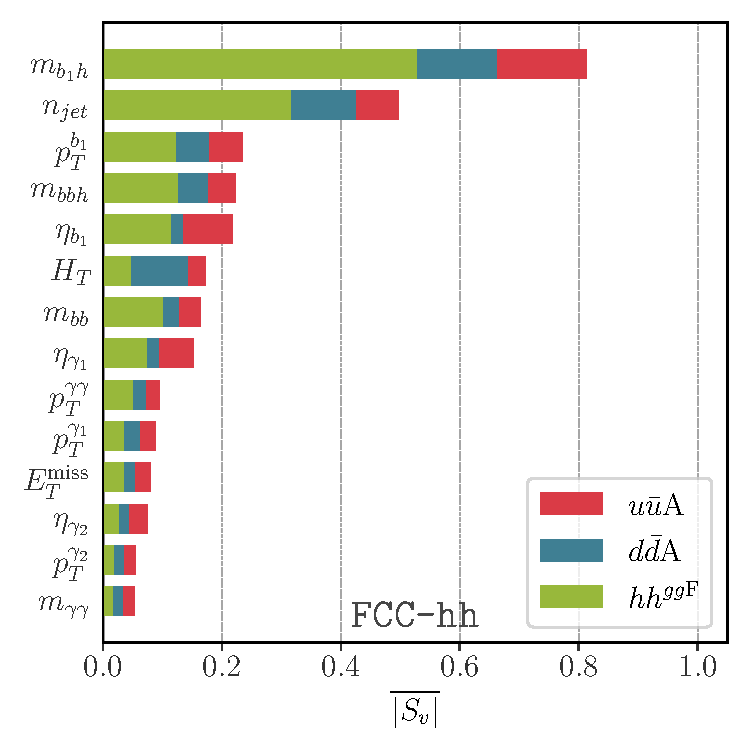
\includegraphics[width=0.45\linewidth]{fig/FCC-hh-shap-ku-kd-hhsm.pdf}
	\caption{\it Top panels: The hierarchy of variables important for the separation of $\hhtri$ from $\hhint$ events from $\hhbox$, $\QQh$ and $\bbaa$ QCD-QED background at HL-LHC (left panel) and FCC-hh (right panel). Middle panels: The hierarchy of variables important for the separation of $\uuA$ from $\ddA$ events at HL-LHC (left panel) and FCC-hh (right panel). Lower panels: The hierarchy of variables important for the separation of $hh^{gg\rm F}$, $\uuA$ and $\ddA$ events at HL-LHC (left panel) and FCC-hh (right panel). The higher the value of $\overline{|S_v|}$ is, the more important the kinematic variable is in separating the different channels.}
	\label{fig:shap}
\end{figure}
\FloatBarrier

\begin{figure}[h!]
	\centering
	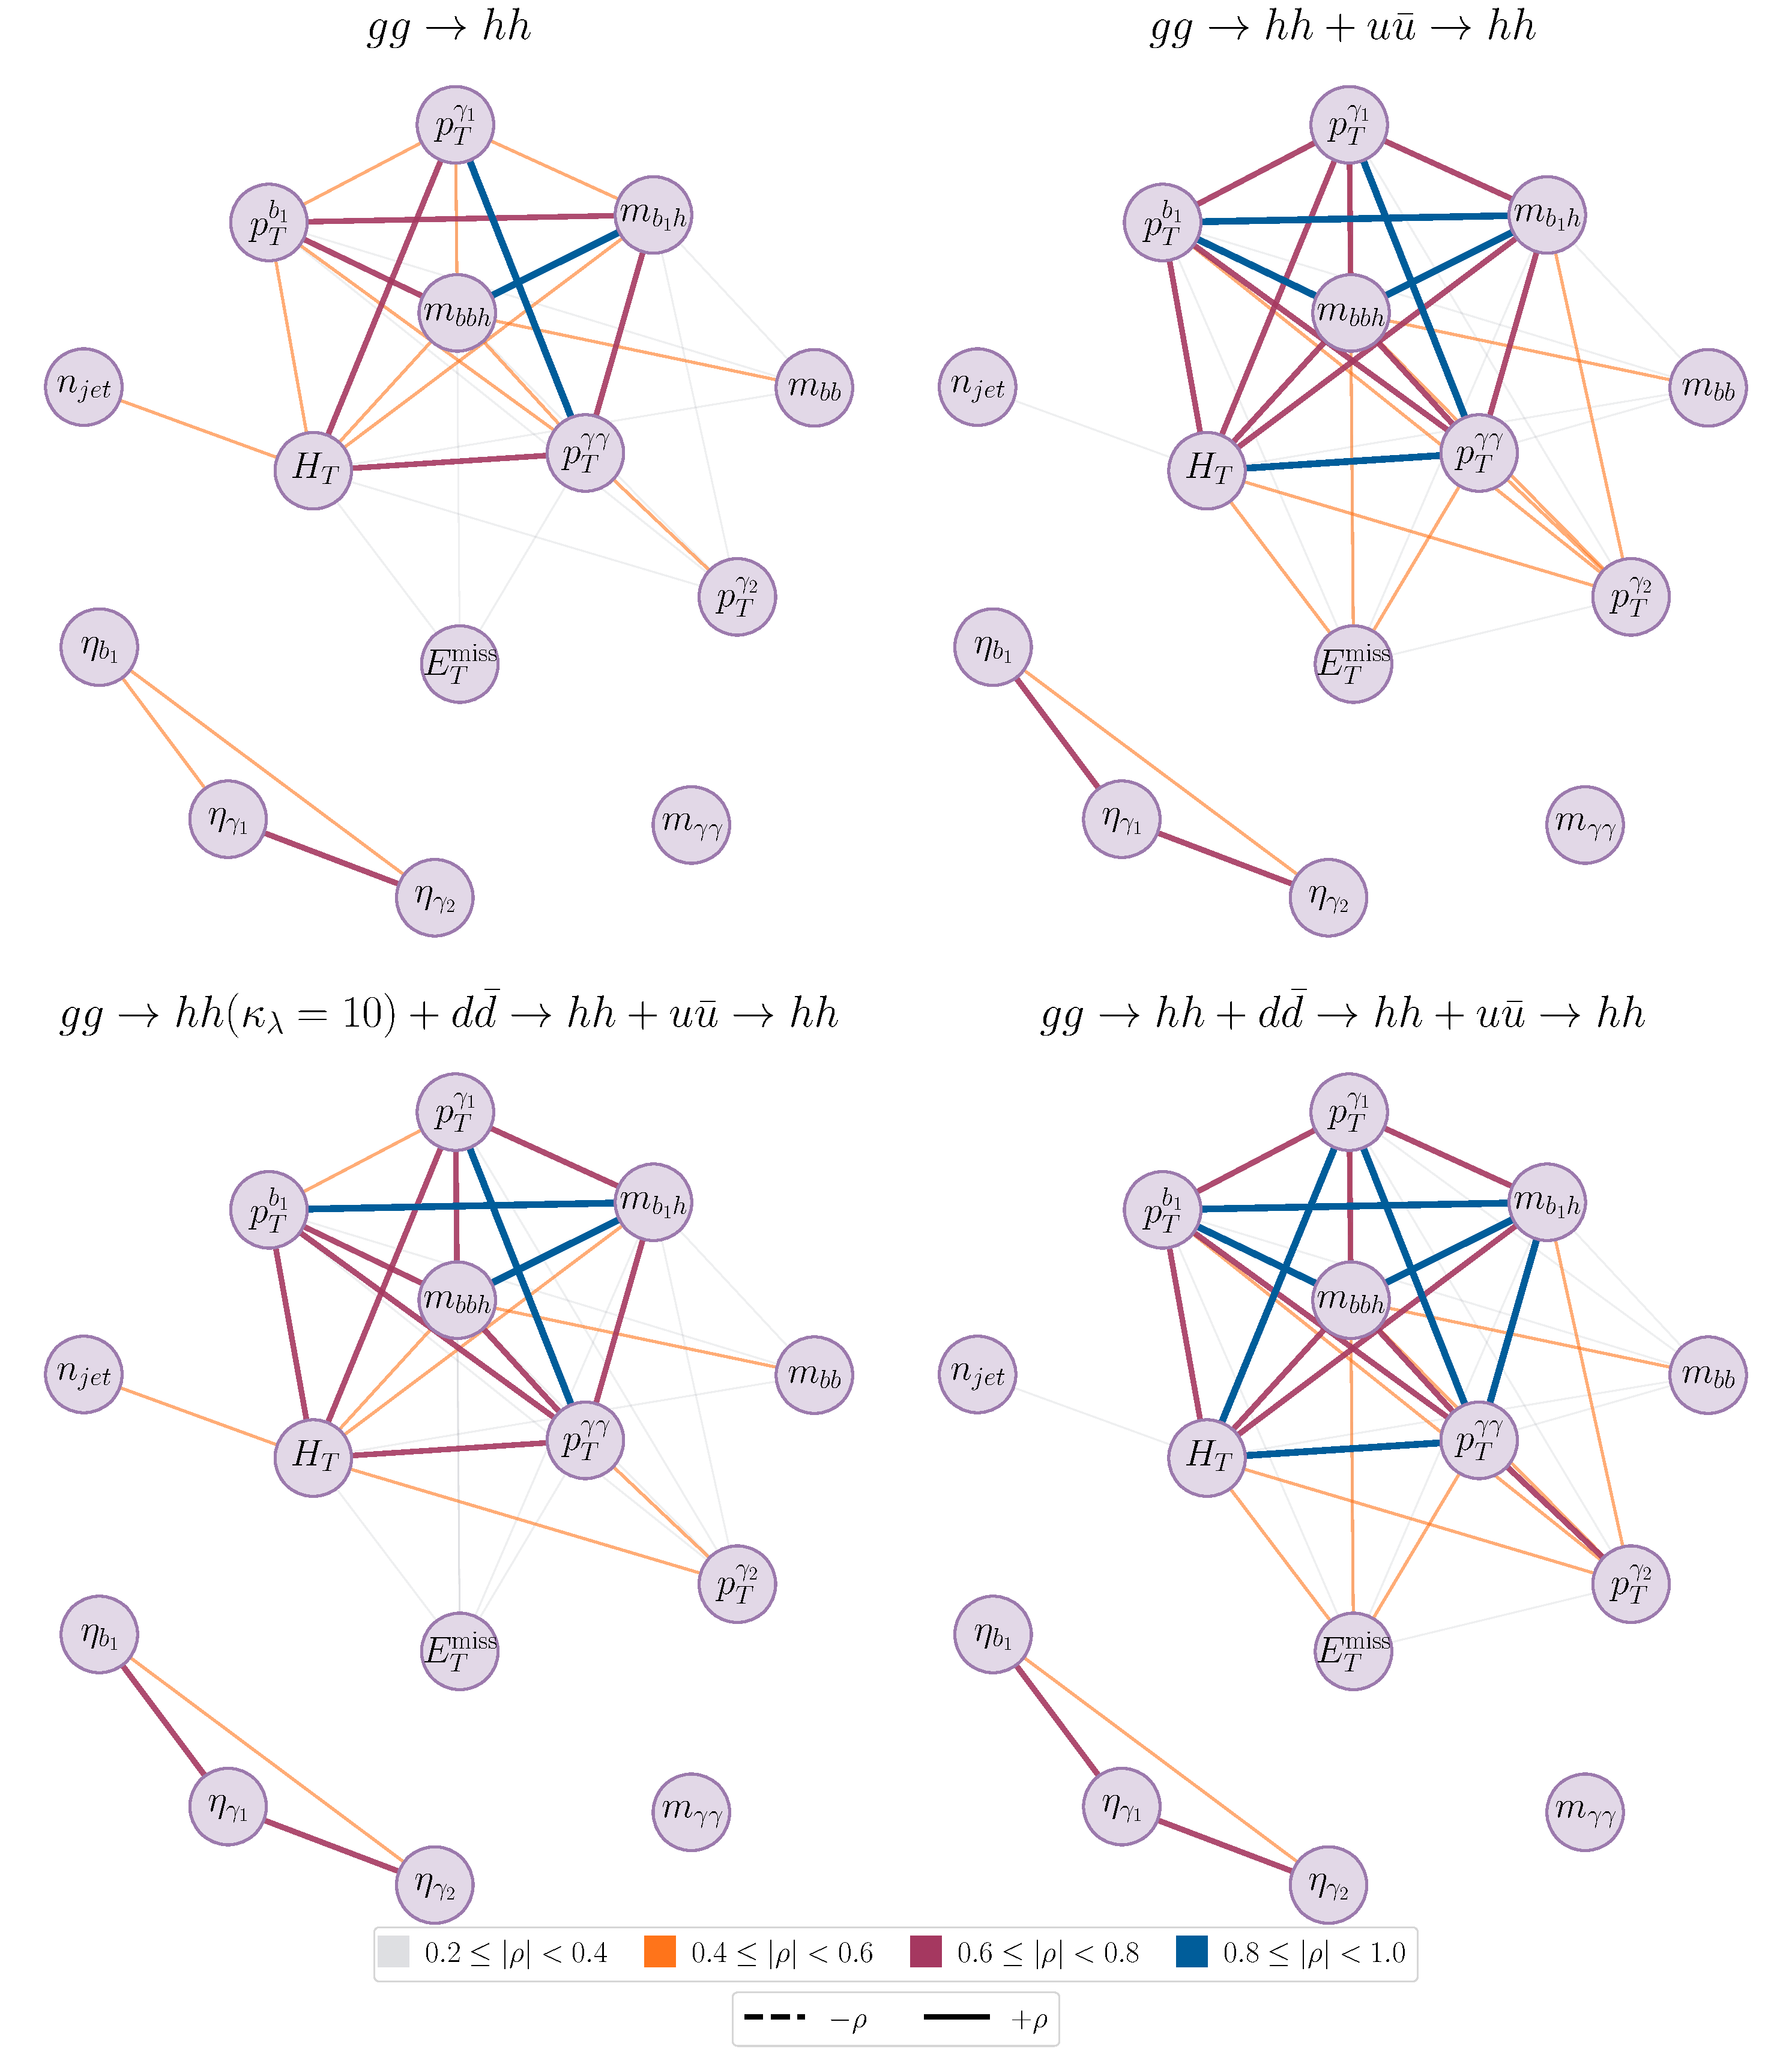
\includegraphics[width=0.9\linewidth]{fig/networks-signal-progression.pdf}
	% 	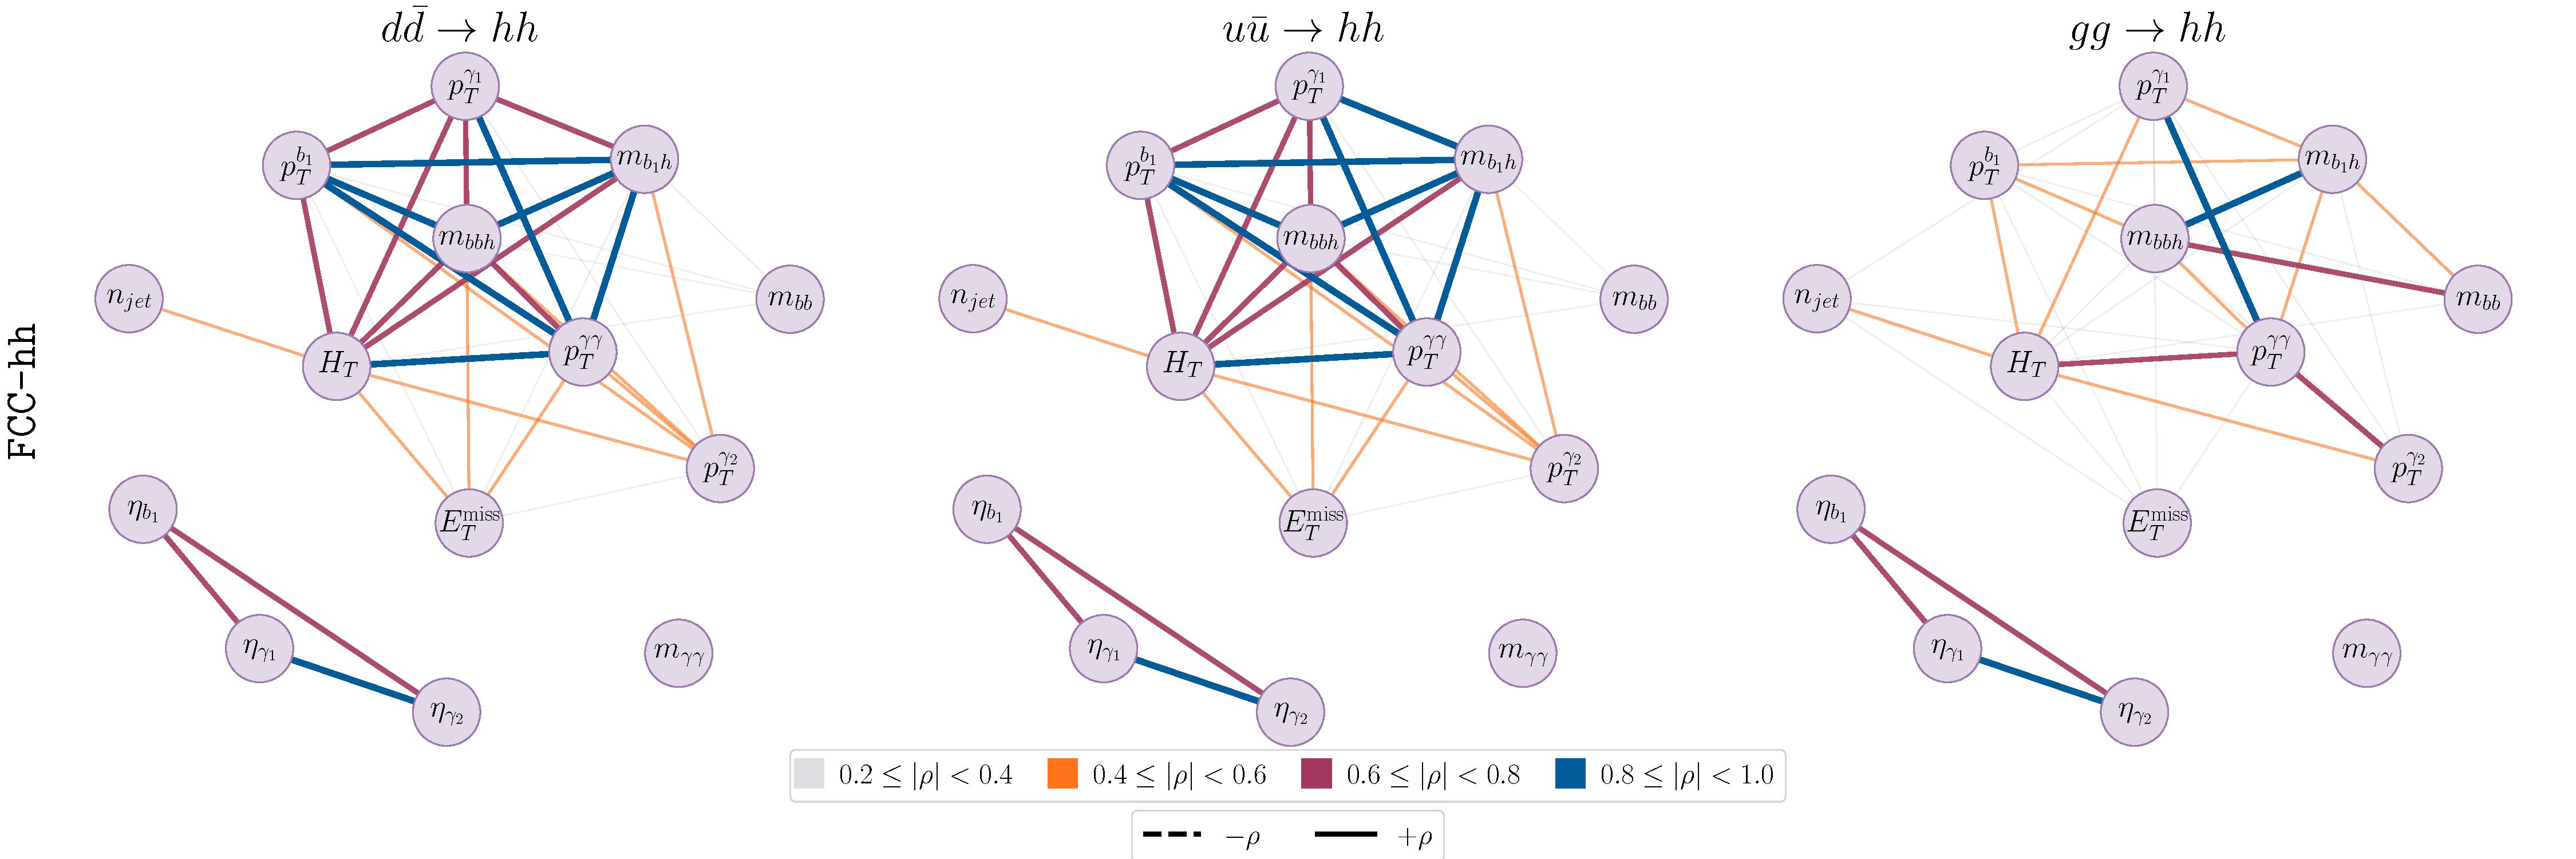
\includegraphics[width=\linewidth]{fig/networks-signal-FCC-hh.pdf}
	\caption{\it Network diagrams visualization of correlations ($\rho$) amongst the kinematic variables used in the analysis. \uline{Top left:} Only the gluon-gluon fusion channel. \uline{Top right:} The $gg$F channel along with the $\uuA$ channel with $\kappa_u=1600$. \uline{Bottom right:} The $\ddA$ channel with $\kappa_d=800$  added to the channels in the top right panel. \uline{Bottom left:} The same channels as in the bottom right panel but with $\kappa_\lambda=10$.}
	% 	\caption{\it A network diagram visualization of correlations ($\rho$) amongst the kinematic variables used in the analysis. The correlation plots in the left panels are generated from the event simulations of $\ddA$, $\uuA$ and $hh^{gg\rm F}$ for HL-LHC at 14 TeV and those in the right panels are for FCC-hh at 100 TeV. The solid and dashed lines signify positive and negative correlations respectively.}
	\label{fig:cor-net}
\end{figure}

For the separation between the two $\qqA$ channels the story is very different. From the middle panels of \autoref{fig:shap} we see that the separation of $\uuA$ and $\ddA$ is truly a multivariate problem. Not surprisingly, the picture is very different for HL-LHC and FCC-hh. The differences between the two channels are driven by the differences in the parton distribution functions (PDF) of the up and down quarks. Since the PDF for the quarks change significantly from 14 TeV to 100 TeV, the variables that effect the separation of the two channels also change. Thus $\overline{|S_v|}$ give us a true picture of how distributions of several kinematic variables determine the separation of different channels that are mostly similar. When comparing the abscissa of the top two panels with the middle two panels one will also notice that $\overline{|S_v|}$ assumes much smaller values in the separation of $\uuA$ and $\ddA$. This clearly shows that the two channels are distributed quite identically and are difficult to separate.

Lastly, in the bottom panels of \autoref{fig:shap} we show the variables that are important in separating the $\qqA$ channels from the $gg$h Higgs pair production channel. The invariant mass of the leading $b-$jet and $h$, $m_{b_1h}$ is the most important variable at both HL-LHC and FCC-hh. However the hierarchy of variables below $m_{b_1h}$ are quite different for HL-LHC and FCC-hh. Both $H_T$ and $p_T^{\gamma\gamma}$ are far less important at FCC-hh than at HL-LHC. This displays the clear advantage that machine learning algorithms have over a cut-and-count analysis where separate cut strategies would have to be built for the two colliders leading to two separate analysis that can, instead, be done with the same framework when using machine learning.

The correlation plots in \autoref{fig:cor-net} show how the linear correlations amongst the variables evolve when different channels are added. The top left panel are events sampled from the $gg$F distribution. One can already see a clustering in some of the variables related to momenta and invariant mass. The other cluster is of the pseudorapidity of the particles in the final state. This correlation structure evolves when one adds the $\uuA$ channel when $E_T^{\rm miss}$ gets connected to the upper cluster in the top right panel. The correlation is now stronger between $\eta_{\gamma_1}$ and $\eta_{b_1}$ and several correlations in the upper cluster are much stronger too. The change in the correlations continue as one keeps adding channels as can be seen from the bottom right and bottom left panels. It is the capture of this change in the correlations (and higher-order correlations) that enhances the capabilities of the machine learning algorithms to distinguish between the various channels. While $m_{\gamma\gamma}$ by its shape alone allows for the separation between $\bbaa$ and the other channels, the correlations between the other kinematic variables aid in the separation of the channels with one or two Higgs in the final state. 




% The correlation plots in \autoref{fig:cor-net} confirm the interplay of variables that the Shapley value plots in \autoref{fig:shap} highlight. The network diagrams are produced with the simulation for both HL-LHC and FCC-hh. \rg{not sure what this sentence should tell me.} It can be seen by comparing the right panels with the left and middle panels that the correlation structure of the upper cluster of variables is markedly different for $hh^{gg\rm F}$ than for $\qqA$. In addition, the lower ``$\eta$'' cluster also shows difference in correlations for HL-LHC. Comparing with the Shapley value plots in the lower panels of \autoref{fig:shap} we understand why $m_{b_1h}$ is the two most important variables that allow for separating $\qqA$ from $hh^{gg\rm F}$. \rg{since it is the most correlated one?} In addition, it should be noted that the separation of the three channels is realized in a truly multivariate manner as several of the variables have comparably large $\overline{|S_v|}$. This lets us understand why the BDT performs so much better over a traditional cut-based analysis where only a few variables cut in an uncorrelated manner would have been considered.


%%%%%%%%%%%%%%%%%%
\section{Summary}
\label{sec:Sum}
%%%%%%%%%%%%%%%%%%
In this work we walk through an analysis of how kinematic shapes can be used to glean information about the nuances of various production modes with the same final states but deformed differentially by the existence of degrees of freedom beyond the Standard Model. We show that this information can be extracted by using an interpretable machine learning framework which is not only very effective separating these differences in kinematic shapes, but also yields itself to interpretations in terms of physics that is know and well understood. The example we chose is Higgs pair production in the $b\bar{b}\gamma \gamma$ final state.
We emphasized that probing Higgs pair production is an important next step for an understanding of the model underlying the fundamental interactions of particles and hence a potential gateway to new physics. We show that even beyond the trilinear Higgs couplings, the light-quark Yukawa couplings can be probed through this production mode. In fact, the $\qqA$ channel opens up only in the presence of BSM physics and well motivated models of new dynamics bring about the simultaneous modification of the trilinear Higgs coupling and the light-quark Yukawa couplings. Indeed, we motivated our study by showing that in different frameworks large modifications of the light quark Yukawa couplings can be obtained. Knowing the difficulty of measuring these couplings we propose an interpretable machine learning framework that significantly outperforms traditional cut-based analyses.

%<Put in some stuff about the models> \rg{I would not since we do not work in concrete models but I modified a bit before.}

As opposed to using black-box models, the interpretable framework allows us to gain physics insights into how signal and background separation can be brought into effect, pointing to kinematic variables like $H_T$ and $m_{\gamma\gamma}$ as being important variables that instrument this separation. As a result we find enhanced sensitivities to $C_\phi$ or $\kappa_\lambda$ that quantify the modification to the Higgs trilinear coupling. Furthermore, we see that the measurement of the light-quark Yukawa couplings is aided by using the methods we advocate bringing about far greater sensitivities than would be possible with a cut-based analysis at the HL-LHC and the FCC-hh. The advantage of using an interpretable framework using Shapley values is that it provides added confidence to the robustness of the multivariate analyses that we perform using simulated data.

The salient results of this work are:
\begin{itemize}
	\itemsep0em
	\item The modification of the Higgs trilinear coupling can be measures at $\mathcal{O}(1)$ precision at the HL-LHC and at $\mathcal{O}(1\%)$ precision at the FCC-hh. 
	\item The rescaling of the light-quark Yukawa couplings, $\kappa_u$ and $\kappa_d$, can be measured to $\mathcal{O}(100)$ at the HL-LHC and $\mathcal{O}(10)$ at FCC-hh. This translated to $C_{u\phi}$ and $C_{d\phi}$ constrained at $\mathcal{O}(10\%)$ at the HL-LHC and $\mathcal{O}(1\%)$ at FCC-hh.
	\item The measurement of $C_\phi$, or $\kappa_\lambda$, is significantly diluted once the light-quark Yukawa couplings are allowed to vary. Hence, in a joint fit, the bounds on $C_\phi$ are much weaker. 
	\item There are theoretical models that motivate the simultaneous modification of the trilinear Higgs coupling and the light-quark Yukawa couplings. Hence, the dilution of the bounds on $C_\phi$ due to the presence of NP in the light-quark Yukawa sector should be taken into consideration in future phenomenological extraction of $C_\phi$.
	\item The bounds obtained with the interpretable machine learning framework that we use not only outperforms cut-based analyses by far, but also allows for physics insights into kinematic distributions of the various channels that helps distinguish them in an experiment.
\end{itemize}

In conclusion, we stress that the interplay between the Yukawa sector and the Higgs trilinear coupling is non-trivial and requires careful consideration. Future experiments at the HL-LHC and FCC-hh will bring significant improvements in the sensitivities to $C_\phi$, $C_{u\phi}$ and $C_{d\phi}$ through the Higgs pair production channel. In particular, the bounds on the light-quark Yukawa couplings from Higgs pair production can possibly be the most stringent bounds amongst all other experimental probes of the light quark Yukawa couplings.

%\rg{I hope no one is upset with me saying this but at the moment the paper reads at too many different styles. I think we should try to unify this a bit. I did not do it only when I felt something was unclearly explained.}



%%%%%%%%%%%%%%%%%%%
%\appendix
%%%%%%%%%%%%%%%%%%%

%%%%%%%%%%%%%%%%%%%%%%%%%%%
%\section{$\kappa$ formalism}
%\label{sec:kappa}
%%%%%%%%%%%%%%%%%%%%%%%%%%%

% It is common to quote the constraints on the Higgs couplings in terms of rescaling to the SM coupling prediction, typically denoted by $\kappa$:
% \begin{equation}
	%     \kappa = \frac{g_h}{g_h^{\mathrm{SM}}}\,.
	% \end{equation}
% If the new physics contributions do not generate new Lorentz structures there is a possible translation between the Wilson coefficients in the SMEFT Warsaw basis, and the $\kappa$ formalism. In particular, taking the rescaling of the trilinear coupling, $\kappa_\lambda$, the translation is given by
% \begin{equation}
	%     \kappa_\lambda = 1-\frac{v^4}{m_h^2} \frac{C_\phi}{\Lambda^2}+3 c_{\phi,\mathrm{kin}},
	% \end{equation}
% where $c_{\phi,\mathrm{kin}}$ is given by
% \begin{equation}
	%   c_{\phi,\mathrm{kin}} = \left( C_{\phi\Box} -\frac{1}{4} C_{\phi D}\right) \frac{v^2}{\Lambda^2}.
	% \end{equation}
% The latter Wilson coefficients modify all the Higgs couplings, and are strongly constrained by electroweak precision observables (e.g.~the $T$ parameter constrains $C_{\phi D}$). Therefore, we set~$c_{\phi,\mathrm{kin}}=0$.\\
% A similar relation exists for the rescalings of the quark Yukawa couplings~$\kappa_q$
% \begin{equation}
	%   \kappa_q = 1+c_{\phi,\mathrm{kin}}- \frac{v^3}{\sqrt{2}m_q}\frac{C_{q\phi}}{\Lambda^2}.
	% \end{equation}
% However, one should be careful while interpreting results quoted in terms of Wilson coefficients in the SMEFT framework extracted from di-Higgs, multi-Higgs or multi-vector bosons searches, as these results include couplings that are not present in the SM. For example, the $hh q\bar{q}$ coupling, though being linearly related to the quark Yukawa coupling $h q\bar{q}$, is not a rescaling of any SM Higgs coupling as has been discussed in \autoref{sec:addconst}. With this in mind, one can strictly remain within a linear EFT and link the rescaling of the quark Yukawa, $\kappa_q$, to the~$hh q\bar{q}$ coupling through
% \begin{equation}
	%   g_{hhq\bar{q}}^{\mathrm{linear-EFT}} = -\frac{3}{2}\frac{1-\kappa_q}{v} \, g_{h q\bar{q}}^{\mathrm{SM}}.
	% \end{equation}
% This relation will no longer hold once a non-linear EFT is used. Hence, the $\kappa$-formalism, in a strict sense, is not  applicable to multi-Higgs studies.


%%%%%%%%%%%%%%%%%%%%%%%%%%%%%%%%%%%%%%%
\section{Discussion of theoretical and systematic uncertainties}
\label{sec:errors}
%%%%%%%%%%%%%%%%%%%%%%%%%%%%%%%%%%%%%%%

\begin{figure}[h!]
	\centering
	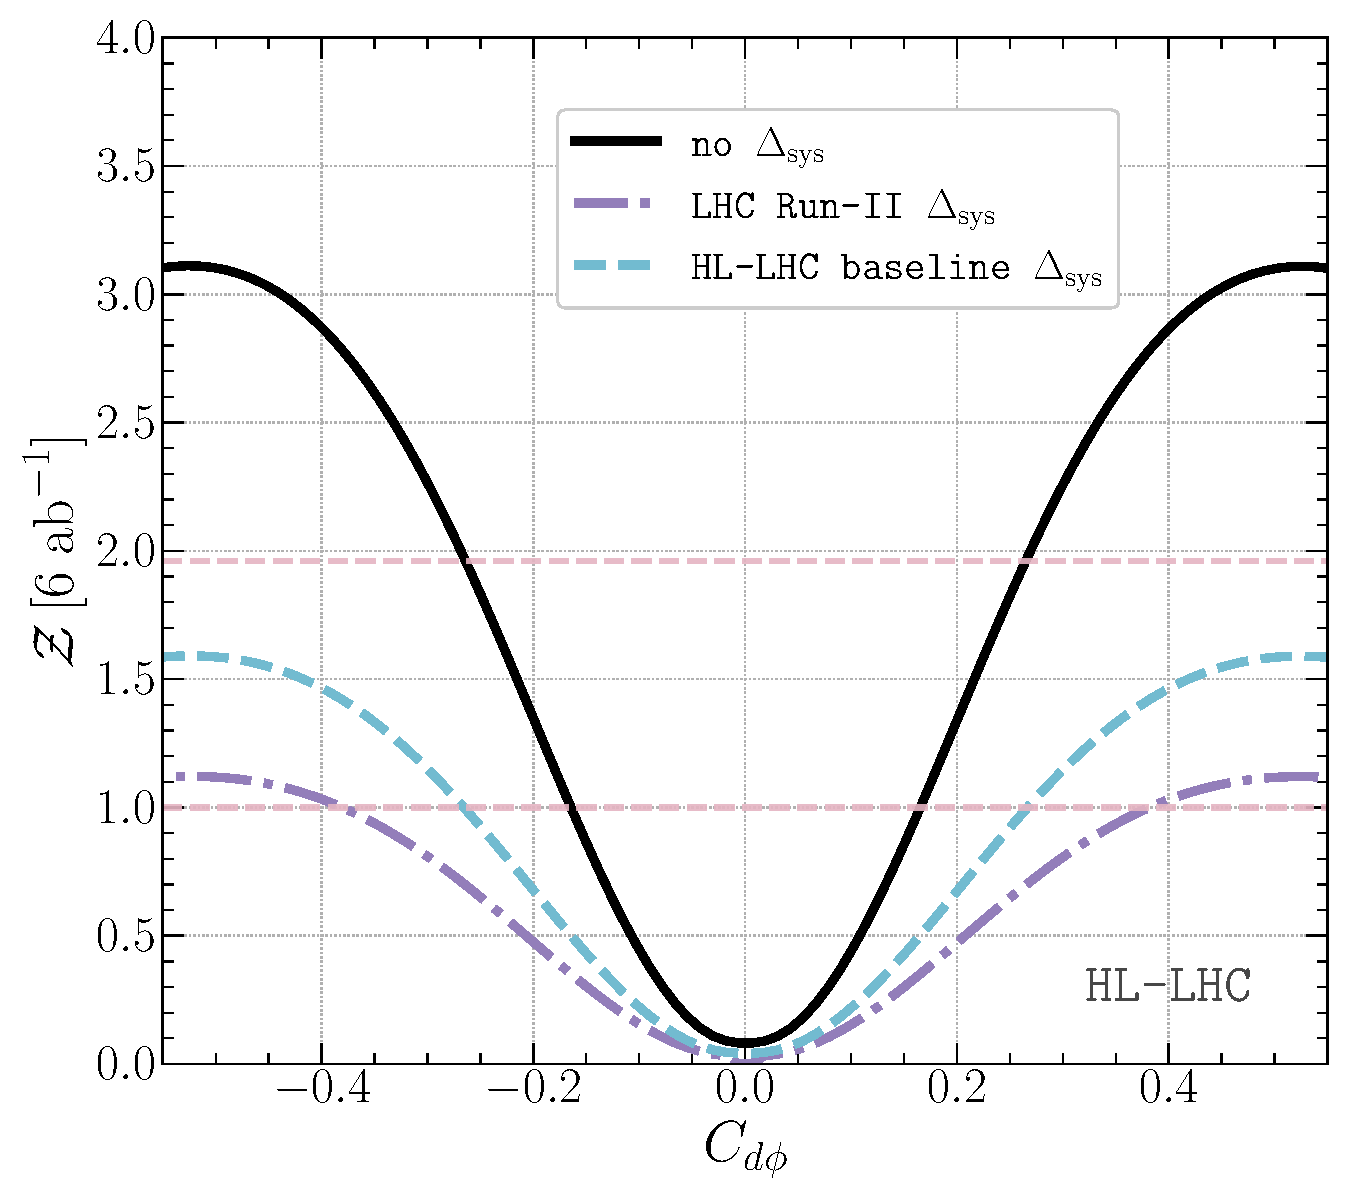
\includegraphics[width=0.4\linewidth]{fig/kd-systematics-HL-LHC.pdf}
	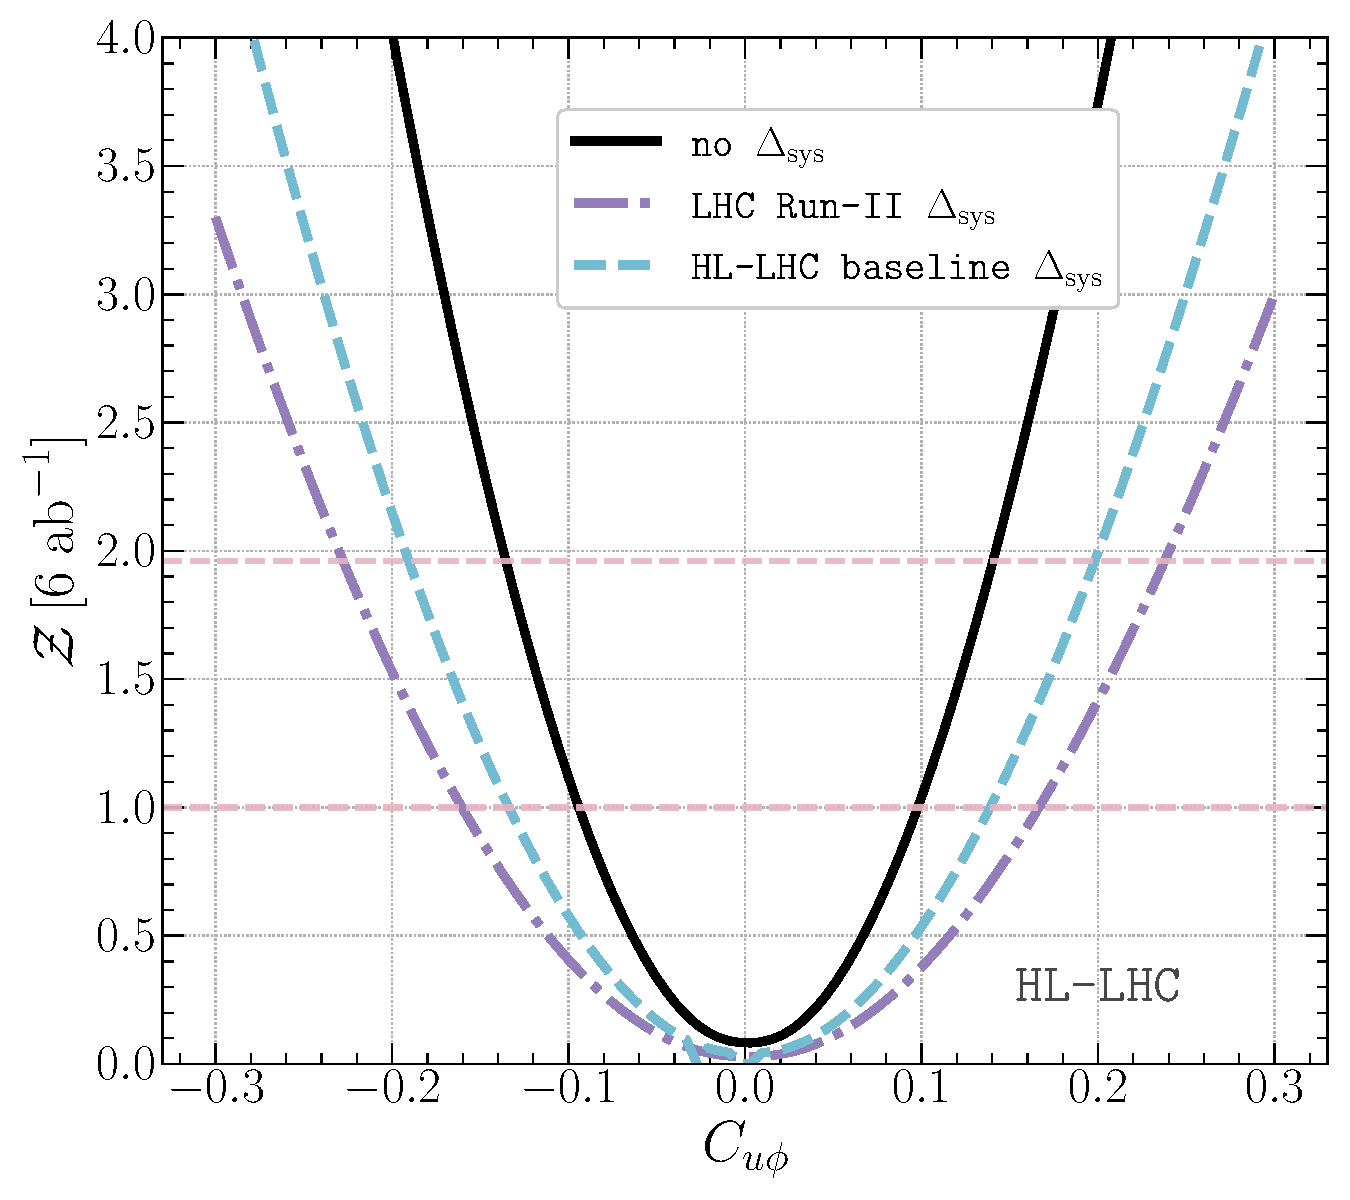
\includegraphics[width=0.4\linewidth]{fig/ku-systematics-HL-LHC.pdf}
	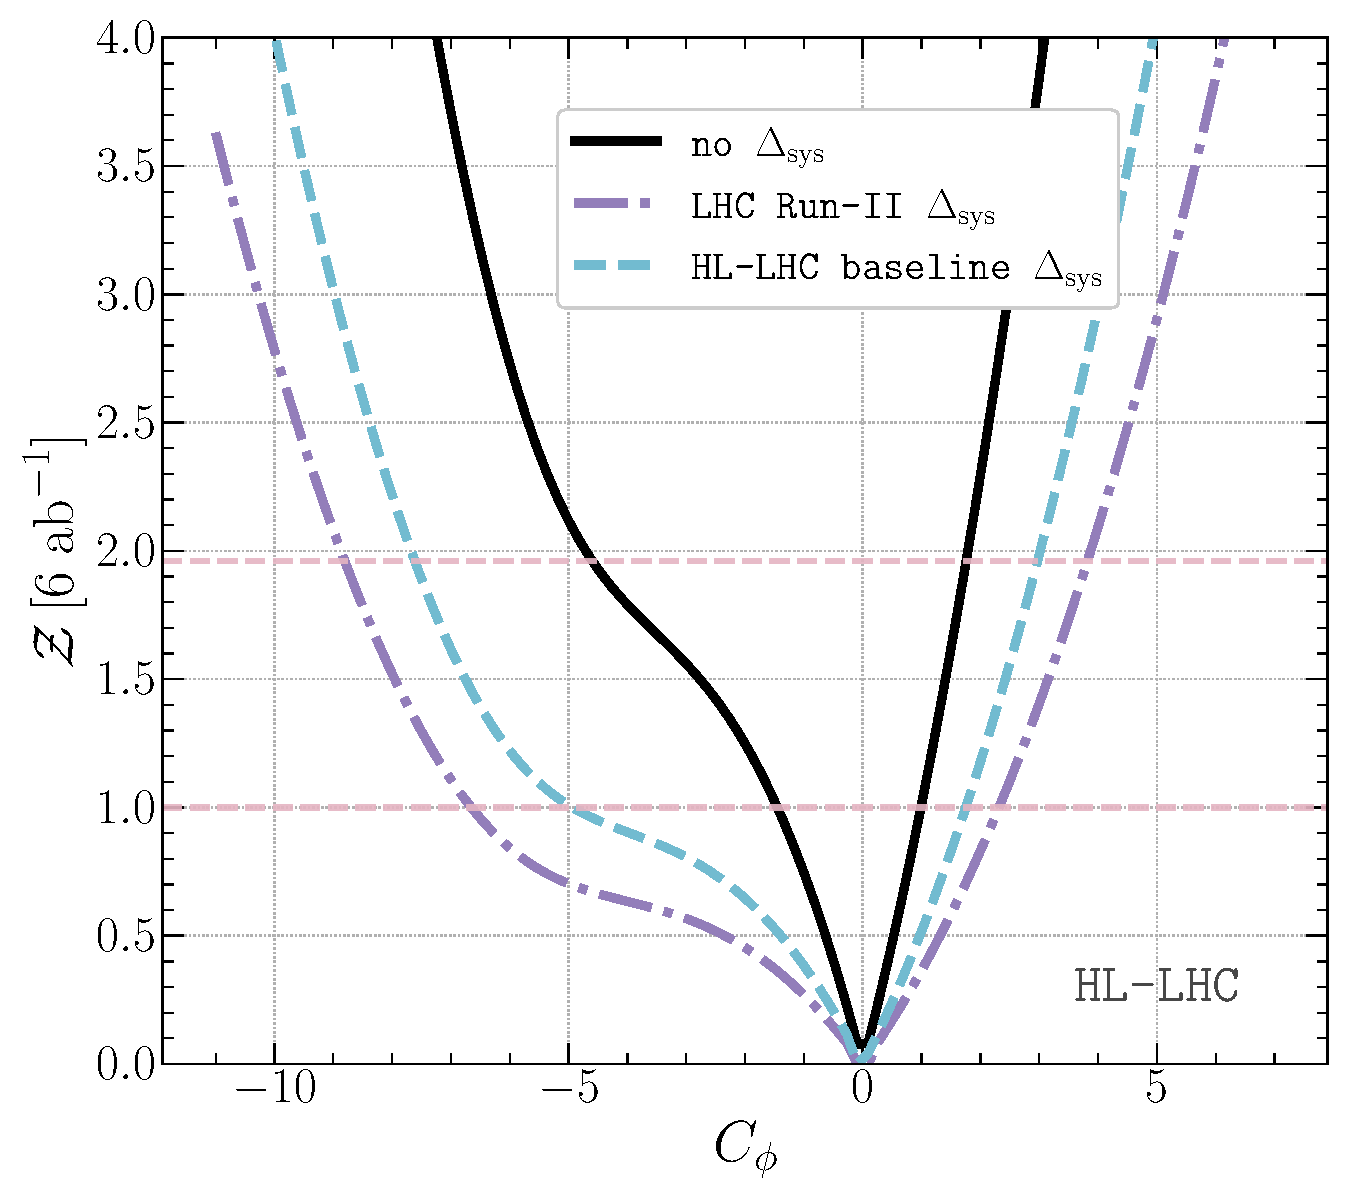
\includegraphics[width=0.4\linewidth]{fig/kl-systematics-HL-LHC.pdf}
	\caption{\it The significance~$\mathcal{Z}$ from a single parameter fit for $C_{d\phi}$ (upper left panel) , $C_{u\phi}$ (upper right panel) and $C_\phi$ (lower center panel) for the HL-LHC with  no systematic uncertainties (black) and two ansätze for systematic uncertainties. The first is the current Run-II $8.2\%$ in violet and the HL-LHC baseline $5.3\%$ estimated by ATLAS in blue, including theoretical uncertainties without top mass renormalisation scheme.}
	\label{fig:systematics}
\end{figure}


% In general, it is difficult to accurately predict the systematic uncertainties for an analysis before it is conducted. This becomes more challenging when one wants to estimate such uncertainties of a future run of a collider or a whole new collider that has not been yet constructed. Therefore, we do not discuss the potential systematic uncertainties for the FCC-hh, and try to give only a rough estimate on the expected systematic uncertainties for the HL-LHC.

%Theoretical uncertainties play the major role in the HL-LHC di-Higgs search uncertainty. The current uncertainty estimate of the SM gluon fusion process at NNLO is ${}^{+6\%}_{-23\%}$ for $\sqrt{s}=14\text{ TeV}$ and ${}^{+4\%}_{-21\%}$ for $\sqrt{s}=100\text{ TeV}$ \cite{Baglio:2020wgt}. 
%The largest part of the uncertainty stems from the uncertainty regarding the renormalization scheme choice of the top quark mass. This uncertainty can for the moment only be estimated at NLO since no full mass dependent results at NNLO are available. While we have used in our analysis only the NLO predictions \rg{I wrote this but I think we should normalise to the best prediction!}, the NNLO results are available only in an approximation called ``FTapprox" \cite{Grazzini:2018bsd} in which the NLO matrix elements are computed in full top mass dependence as well as the double real radiation contributions. The uncertainties show also a dependence on the value of the trilinear Higgs self-coupling, see \cite{Baglio:2020wgt}. 

%While we have used in our analysis the $\bar{q}q$A at NLO QCD where the combined scale and PDF$+\alpha_s$ uncertainty amounts to $\pm 9\%$, the NNLO QCD corrections could be translated from the bottom annihilation to Higgs pairs case \cite{Ajjath:2018ifl} where we estimate the uncertainty to be $<5\%$.
%Finally, we note that when computing higher order corrections to the $\bar{q}q$A channel a separation between $\bar{q}q$A and ggF is no longer possible since by including real radiation the processes have the same initial and final state.  This issue has for instance be discussed for the case of $b\bar{b}h$ in \cite{Pagani:2020rsg}.

%\rg{Should we write something on the EFT truncation uncertainty?}
%\la{We did not truncate here, we have used quadratic SMEFT for both $C_{q\phi}$ and $C_\phi$}
%\rg{In our analysis we did not really use the best predictions, right? It should be noted that  That would include for instance doing a differential K-factor. I am not sure that we should go over this but at the same time discuss the theoretical uncertainties in detail.}\la{I agree, but it is more complicated than that. We use many distributions that their NLO or NNLO were not published and unlike $b \bar{b} h$, the k-factor is not approx. flat across the distributions so we could only do k-factor rescaling at the end.}

In this section we present an estimate of the systematic uncertainties that can affect the measurements discussed in this work at the HL-LHC. We do not present these estimates for the FCC-hh for lack of sufficient information or the ability to project such uncertainties far into the future. We use two scenarios for systematic uncertainties: the first is a $8.2\%$ uncertainty which corresponds to the current systematic uncertainty that ATLAS has reported for their Run-II search for Higgs pair production~\cite{ATLAS-CONF-2021-016}. The second scenarios is the ATLAS HL-LHC baseline systematic uncertainty of $5.3\%$ reported in~\cite{ATL-PHYS-PUB-2018-053}. For LHC run-II, statistical uncertainties remain the dominant part of the uncertainty budget for di-Higgs analysis. Regarding the systematic uncertainties, experimental sources remain the dominant part in comparison to the theoretical ones.  The story flips for the HL-LHC where the main source of uncertainties is expected to be coming from theoretical uncertainties. The current theoretical uncertainty estimate of the SM gluon fusion process at NNLO is ${}^{+6\%}_{-23\%}$ for $\sqrt{s}=14\text{ TeV}$ and ${}^{+4\%}_{-21\%}$ for $\sqrt{s}=100\text{TeV}$~\cite{Baglio:2020wgt}. The largest part of the uncertainty stems from the uncertainty due to the renormalization scheme choice of the top quark mass. This uncertainty can, for the moment, only be estimated at NLO since no full mass dependent results at NNLO are available. Moreover, the top quark mass renormalization scheme uncertainty is not included in the estimated HL-LHC (nor LHC Run II) uncertainties schemes that we have considered. 

In \autoref{fig:systematics} we show the significance~$\mathcal{Z}$ for the three Wilson coefficient, $C_\phi$, $C_{u\phi}$ and $C_{d\phi}$, at the HL-LHC from single parameter fits with no systematic uncertainties (black), LHC Run-II (violet) and HL-LHC baseline (blue) systematic uncertainties ansatze. We observe that for the current Run-II ansatz, the bounds for all three Wilson coefficients is diluted by 100\% or more. As for the HL-LHC baseline, the bounds are diluted by $\sim$ 70\%. However, it should be noted, that both systematic uncertainties scenarios are rather conservative. It is likely that the HL-LHC detector upgrade and new theoretical developments in higher-order corrections to di-Higgs cross-section will reduce the systematic uncertainties from the baseline. 

%%%%%%%%%%%%%%%%%%%%%%%%%%%
\section{Light-quark Yukawa and Self Coupling at Future Lepton Colliders}
\label{sec:Lep}
%%%%%%%%%%%%%%%%%%%%%%%%%%%
Future high energy lepton colliders~\cite{Charles:2018vfv,Bambade:2019fyw,CEPCStudyGroup:2018ghi} offer further alternative and clean signals for measurement of Higgs properties. 
%Among the many advantages, the Higgs decay to flavor-tagged jets, especially $c$ and $b$ quarks will benefit from the clean environment at a lepton collider and reach sensitivities improved by orders of magnitude of (1.8\% and 1.3\% at 250 GeV 5ab$^{-1}$) compared with ($\mathcal{O}(1)$ and 3.6\%) at the HL-LHC inclusive $\kappa$ fit or kinematic study~\cite{deBlas:2019rxi,Bishara:2016jga}. % We are not conserned with c and b 
For example, Higgs decays to ``un-tagged'' light jets including $u,d,s$ quarks can be further disentangled from $H\to gg$ using event shape analysis~\cite{Gao:2016jcm} and can reach a sensitivity of $\kappa_d \approx 90$ and $\kappa_u \approx192$ at 250 GeV with 5ab$^{-1}$ data compared with a sensitivity of $\kappa_d \approx 470$ and $\kappa_u \approx900$ at the 6ab$^{-1}$ HL-LHC~\cite{Carpenter:2016mwd,Soreq:2016rae}.

The sensitivity to Higgs self-coupling comes indirectly for center of mass energy below 250 GeV from the precision measurement of the $Zh$ production channel ($\delta \kappa_\lambda$  ($1\sigma$)~$0.4$ at 250 GeV), and at 500 GeV directly from the $Zhh$ channel ( $\delta \kappa_\lambda$  ($1\sigma$)~$0.27$ at 500 GeV), and from vector boson fusion like production to $hh\nu\nu$ when 1 TeV or higher energy scales are available ($\delta \kappa_\lambda$  ($1\sigma$)~10\% at 1 TeV). The prospective sensitivity depends on the collider setup, mainly the integrated luminosity and polarization of initial lepton beams. Given the updated prospects of future machine designs~\cite{deBlas:2019rxi}, 
we list a short summary in \autoref{tab:exp_yqyl} of the expected sensitivities on the individual parameters in the $\kappa$ framework. These numbers are all assuming one-parameter fits in $\kappa$ or (translated from) SMEFT framework. No simultaneous fit including both $\kappa_q$ and $\kappa_\lambda$ (or using the corresponding SMEFT operators) have been performed yet. 


%\begin{table}[]
%    \centering
%   {\footnotesize
	%   \begin{tabular}{c|c|c|c|c}
		%   \hline
		%         \ &  $\kappa_u$ &  $\kappa_d$ & $y_s/y_b^{\rm SM}$ & %$\lambda_3/\lambda_3^{\rm SM}$  ($1\sigma$) \\ \hline
		%        300 fb$^{-1}$ (LHC) & $ 0.36$ \cite{Soreq:2016rae} (820) & $ %0.41$ \cite{Soreq:2016rae} (430) &  - & -\\ 
		%     3000 fb$^{-1}$ (HL-LHC) &  0.48 \cite{deBlas:2019rxi} &  0.5 %\cite{deBlas:2019rxi} & $ 0.58$ \cite{Bishara:2016jga} (30)& %$50\%$ \cite{deBlas:2019rxi}\\
		%        250 GeV 1 ab$^{-1}$ (ILC) & 0.28*\cite{deBlas:2019rxi} & %0.16*\cite{deBlas:2019rxi}& & \\
		%       240GeV 5ab$^{-1}$ (CECP/FCC) & $0.09$ \cite{Gao:2016jcm} (204) & %$0.09$ \cite{Gao:2016jcm} (94) & $ 0.09$ \cite{Gao:2016jcm} (4.8) %& 100\% (Indirect\cite{DiVita:2017vrr})\\
		%         350 GeV 1.5 ab$^{-1}$ (FCC) & 0.2*\cite{deBlas:2019rxi} & %0.12*\cite{deBlas:2019rxi} & & 40\% %(Indirect\cite{DiVita:2017vrr})\\ 
		%      500 GeV 4 ab$^{-1}$ (ILC) & 0.2*\cite{deBlas:2019rxi} & %0.13*\cite{deBlas:2019rxi}& & 27\% \cite{Bambade:2019fyw} \\
		%       1 TeV 8 ab$^{-1}$ (ILC) & 0.14*\cite{deBlas:2019rxi} & %0.12*\cite{deBlas:2019rxi} & & 10\% \cite{deBlas:2019rxi} \\
		%  %       100 TeV 30 ab$^{-1}$ (FCC-hh) & 0.1*\cite{deBlas:2019rxi} & %0.14*\cite{deBlas:2019rxi} & & 5\% \cite{deBlas:2019rxi}\\
		%      10 TeV 10 ab$^{-1}$ (Muon) & & & & 3\% \cite{deBlas:2019rxi}\\ %\hline
		%     \end{tabular}
	%\caption{Prospective light-quark Yukawa and Higgs self-coupling %sensitivities at future lepton colliders. The light-quark Yukawa %bounds are 95\% CL, while the self-coupling bounds are $1\sigma$ or %68\% CL sensitivity reach. The starred (*) numbers are translated from %one-parameter SMEFT fit results. The translation is done by taking %$\delta y_q = \delta(\frac{c_{qH}}{\Lambda^2}) \frac{v^2}{2}$, and %normalizing to the SM b-Yukawa coupling around Higgs mass %$m_b(\mu=M_H) = \frac{y_b^{\rm SM}v}{\sqrt{2}}= 2.7$ GeV.}
	%  \label{tab:exp_yqyl}
	%   }
%\end{table}


\begin{table}[t!]
	\centering
	{\small
		\begin{tabular}{cccc}
			\toprule
			Collider &  $|\kappa_u|$ &  $|\kappa_d|$  & $\delta \kappa_\lambda$  ($1\sigma$) \\ \midrule
			%250 GeV 1 ab$^{-1}$ (ILC) & 343*\cite{deBlas:2019rxi} & 91*\cite{deBlas:2019rxi} &-- \\
			240GeV 5ab$^{-1}$ (CECP/FCC) & 192 \cite{Gao:2016jcm}  & 90 \cite{Gao:2016jcm}   & 100\% (Indirect\cite{DiVita:2017vrr})\\
			350 GeV 1.5 ab$^{-1}$ (FCCee) & 310\cite{deBlas:2019rxi} & 140\cite{deBlas:2019rxi} &  40\% (Indirect\cite{DiVita:2017vrr})\\ 
			500 GeV 4 ab$^{-1}$ (ILC) & 330\cite{deBlas:2019rxi} & 160\cite{deBlas:2019rxi}&  27\% \cite{Bambade:2019fyw} \\
			1 TeV 8 ab$^{-1}$ (ILC) & -- & -- &  10\% \cite{deBlas:2019rxi} \\
			3 TeV 1 ab$^{-1}$ (CLIC) & 430\cite{deBlas:2019rxi} & 200\cite{deBlas:2019rxi} &  10\% \cite{deBlas:2019rxi}\\
			10 TeV 10 ab$^{-1}$ (Muon) & --& --&  3\% \cite{deBlas:2019rxi}\\ \bottomrule
		\end{tabular}
		\caption{\it Prospective light-quark Yukawa and Higgs self-coupling sensitivities at future lepton colliders. The light-quark Yukawa bounds are 95\% CL, while the self-coupling bounds are $1\sigma$ or 68\% CL sensitivity reach.}
		\label{tab:exp_yqyl}
	}
\end{table}

%From ~\cite{Alasfar:2019pmn}, we see that the two could be correlated in di-Higgs observable especially in the SMEFT framework, where contact interaction of $q\bar q HH$ contribution to di-Higgs production become dominant with enhanced light-quark Yukawa coupling. Thus a separation of sensitivity to the various channel in the di-Higgs signal is essential to disentangle the different source of NP contribution from expected future collider data. \rg{I am not sure what the last few lines have to do with a future lepton collider. I have the feeling that the major correlation in this case would come from the fact that the light Yukawas would modify the decay rates so this would need to be considered in fits.}